
\documentclass{lmcs}

\usepackage[T1]{fontenc}
\usepackage[utf8]{inputenc}
\usepackage{amssymb,mathtools,booktabs}
\usetikzlibrary{arrows.meta,calc,positioning}
\usepackage{xurl}
\microtypesetup{expansion=false}

\urlstyle{tt}
\Urlmuskip=0mu plus 2mu\relax
\DeclareUrlCommand\AgdaPath{\urlstyle{tt}}

\newcommand{\N}{\mathbb{N}}
\newcommand{\Z}{\mathbb{Z}}
\newcommand{\U}{\mathcal{U}}
\newcommand{\B}{\mathcal{B}}
\newcommand{\Lcal}{\mathcal{L}}
\newcommand{\Gcal}{\mathcal{G}}
\newcommand{\RawDecl}{\mathrm{RawDecl}}
\newcommand{\Cand}{\mathrm{Cand}}
\newcommand{\Layer}{\mathrm{Layer}}
\newcommand{\NormSig}{\mathrm{NormSig}}
\newcommand{\ObSig}{\mathrm{ObSig}}
\newcommand{\Ix}{\mathrm{Ix}}
\newcommand{\Real}{\mathrm{Real}}
\newcommand{\Prim}{\mathrm{Prim}}
\newcommand{\Der}{\mathrm{Der}}
\newcommand{\PrimClasses}{\mathrm{PrimClasses}}
\newcommand{\Foot}{\mathrm{Foot}}
\newcommand{\Shape}{\Pi_{\!\infty}}
\newcommand{\Supp}{\mathrm{Supp}}
\newcommand{\hcomp}{\mathrm{hcomp}}
\newcommand{\compop}{\mathrm{comp}}
\newcommand{\transp}{\mathrm{transp}}
\newcommand{\OpenExt}{\mathrm{OpenExt}}
\newcommand{\Partial}[2]{\mathrm{Partial}_{#1}(#2)}
\newcommand{\Type}{\mathrm{Type}}
\newcommand{\El}{\mathrm{El}}
\newcommand{\Fib}{\mathrm{Fib}}
\newcommand{\Cext}{C_{\mathrm{ext}}}

\title[Toward Coherence Depth Two]{Toward Coherence Depth Two for Cubical Sealed Extensions}

\author[H.\ Lande]{Halvor Lande}
\address{Independent researcher, Oslo, Norway}
\email{halvor.s.lande@gmail.com}

\keywords{cubical type theory, extension calculus, coherence, univalence}
\subjclass[2012]{Theory of computation~$\rightarrow$~Type theory; Mathematics of computing~$\rightarrow$~Algebraic topology}

\begin{document}

\begin{abstract}
Type-theoretic foundations can grow by sealing globally acting structural
layers: modalities, universe formers, promoted interface packages, and similar
operations whose behavior becomes part of the public core.  Such a layer must
explain how it interacts with already exported structure; we call this residue
its public structural trace.  This paper proves a depth-two theorem for a fixed
cubical sealed-extension calculus.  Unary trace is not enough, because
univalence turns equivalences such as the nontrivial swap of the two-point type
into public paths.  Higher structural trace generated by sealing is not
primitive: it is represented by cubical open-box extension data computed from
lower-arity boundaries.  Consequently the exact realized obligation objects
stabilize at binary trace, and normalized minimal public signatures contain no
primitive structural trace field above binary arity.  Separate full-coupling
hypotheses give a two-step accounting recurrence; the Fibonacci form is only a
constant-payload envelope.  The mechanized development checks the theorem-facing
fixed-calculus stack, the concrete SMod adequacy instance, semantic wrapper
interfaces, case-study fixtures, and the theorem-map/postulate audit; broader
transfer to other cubical foundations remains conditional on the stated
interface.
\end{abstract}
\maketitle

\section{Introduction}

A type-theoretic library can grow in two very different ways.  In the first,
a user defines a new transparent object inside an already fixed foundation.  A
new datatype of trees, for example, need not explain how it interacts with every
old construction in the library before it can be used.  Its dependencies are
local, and the surrounding theory can mostly ignore it.

The second kind of growth is less forgiving.  A foundation can be extended by a
new sealed structural layer: a modality, a universe former, a promoted interface
package, or some other globally acting operation whose public behavior becomes
part of the exported core.  Such an extension is not merely another transparent
term.  Once sealed, it advertises a stable public interface.  It must therefore
explain how it acts on the active structure already present: old type formers,
transport operations, eliminators, computation rules, paths, equivalences, and
comparison data.  This explanatory residue is what we call \emph{public trace}.

The question of this paper is:
\begin{quote}
When a cubical type-theoretic foundation is extended by a sealed, globally acting
structural layer, how much public integration trace must remain primitive after
normalization and opacity?
\end{quote}

The answer proved here is a depth-two theorem for one fixed formal calculus.  In
that calculus, unary trace is not enough: univalence supplies genuine binary
naturality obligations.  But trace above binary arity is not primitive: the
higher structural obligations generated by sealing are cubical open-box extension
problems, and cubical composition and filling compute their missing faces and
fillers.  Thus higher exact obligation factors remain visible in the semantics,
but they disappear from minimal opaque public signatures.

A useful slogan is:
\begin{quote}
Binary trace is necessary; higher structural trace is cubically payable.
\end{quote}

This slogan is deliberately about \emph{structural integration trace}, not about
all higher homotopy in a cubical theory.  The theorem does not say that higher
paths vanish, that user-supplied higher payload is forbidden, or that ordinary
libraries grow according to a fixed recurrence.  It says that, for the sealed
extension calculus studied below, the additional public trace forced by sealing a
globally acting structural layer stabilizes at binary trace.

\subsection{Payload, trace, and the first obstruction}

The first distinction is between \emph{payload} and \emph{trace}.  The payload is
what the new sealed layer contributes: a new operation, modality, universe rule,
or promoted structural package.  The trace is the public evidence that this
payload interacts correctly with the already exported interface.

Consider a small old interface containing two objects \(A\) and \(B\), together
with a comparison
\[
  p : A \simeq B
\]
or, in a univalent presentation, a path obtained from such an equivalence.  Now
seal a new globally acting operation \(X\).  There are several levels of public
obligation.

First, there is unary trace: the extension must say how \(X\) acts on individual
old generators such as \(A\) and \(B\).  This is objectwise information.  Second,
there is binary trace: the extension must say that the action of \(X\) respects
old comparison data such as \(p\).  This is not reducible to two unrelated unary
actions, because \(p\) is part of the old public interface.  A sealed action that
acts correctly on \(A\) and \(B\) separately may still fail to commute with the
public equivalence between them.

The basic lower-bound example is the two-point type.  Univalence turns the
nontrivial boolean swap equivalence into a public path.  A candidate sealed
action may be well formed objectwise but fail the naturality square along this
swap path.  More precisely, transport in the endomorphism family along the
univalent swap path conjugates an endomap by the swap.  The identity endomap is
fixed by this conjugation, while the constant-left endomap is sent to the
constant-right endomap.  Thus the unary fragment can accept objectwise data
whose binary sealing obligation is uninhabited.  Hence unary trace alone cannot
decide admissibility in general.  Binary trace is a real public obligation, not
an accounting artifact.

This is the first half of the depth-two story:
\[
  \text{depth one is insufficient.}
\]
The second half explains why the story stops at two.

\subsection{Why higher structural obligations are different}

At first sight, sealing seems to create an infinite tower.  If unary action must
respect binary comparison data, should binary comparison data itself not satisfy
ternary compatibility laws?  Should those laws not satisfy quaternary laws, and
so on?  This is the familiar shape of coherence problems.

Cubical foundations change the accounting.  Their primitive operations are built
to solve open-box extension problems.  Given a partial boundary of a cube and a
compatible base, cubical composition and filling supply the missing face and the
interior filler.  In a CCHM-style core~\cite{cubical} this is the role of the
Kan operations, together with transport and the interval structure.  The point
of the present paper is that the higher structural obligations generated by
sealing have exactly this open-box form.

The relevant higher obligation is not an arbitrary closed higher-dimensional
choice.  It is a \emph{marginal extension problem}.  The lower-dimensional faces
come from the already exported unary and binary trace, together with normalized
public signatures of previous sealed layers.  What appears as a ternary or higher
coherence field is therefore represented as an open box: a partial boundary, a
compatibility condition, a missing remote face, and a filler.  In the fixed
calculus, this open-box extension object is contractible and substitution-stable.
Its canonical point is computed using cubical composition and filling.

This is the key semantic mechanism.  Higher structural obligations are not
ignored.  They remain present in the exact realized obligation object.  But they
are no longer primitive public data, because the calculus computes them from the
lower-arity boundary.  Equivalently, an explicit higher structural field in a
surface presentation can be replaced by a cubical term built from the displayed
boundary, and then erased from the minimal public signature.

Thus the main theorem has two levels.  At the level of exact realized obligation
objects, higher factors are present but contractible.  At the level of normalized
opaque public signatures, higher structural fields are absent from the primitive
trace count.

\subsection{The fixed calculus proved here}

Let \(C_{\mathrm{ext}}\) be the sealed-extension calculus defined in this paper.
It consists of a CCHM-style cubical core with univalence and Kan
composition~\cite{cubical}, globally acting extension declarations, opaque
public signatures, and a raw adequacy bridge connecting surface presentations to
normalized trace objects.  The definitions of \(C_{\mathrm{ext}}\) are part of
the theorem object.

For an admissible candidate \(X\), write \(\mathrm{Real}_k(X)\) for the exact
realized structural obligation object obtained when public trace is allowed up
to arity \(k\).  Write \(\mu\) for the primitive public trace cost of a normalized
opaque signature.  The central result is:
\begin{quote}
\textbf{Main theorem for \(C_{\mathrm{ext}}\).}
For every admissible candidate \(X\), the exact realized obligation objects
stabilize at binary trace:
\[
  \mathrm{Real}_k(X) \simeq \mathrm{Real}_2(X)
  \qquad (k \geq 2).
\]
Moreover, every \(\mu\)-minimal normalized public signature contains no primitive
structural trace field of arity greater than two.  Unary trace is insufficient in
general, as witnessed by the two-point swap obstruction.
\end{quote}

The theorem should be read as an exact-depth statement for a fixed calculus:
\[
  \begin{gathered}
  \text{binary trace is necessary,}\\
  \text{and binary trace is sufficient for primitive public structural integration.}
  \end{gathered}
\]

\subsection{Scope and non-goals}
\label{subsec:scope-nongoals}

The theorem is intentionally scoped.  It is a theorem about the fixed calculus
\(C_{\mathrm{ext}}\), not a claim that this is the only possible formalization
of sealed cubical extension, nor that every Cubical Agda program~\cite{cubical-agda}
automatically interprets into it.  The result also does not say that all higher
filler spaces in Homotopy Type Theory are contractible.  The contractible
objects are the theorem-facing structural open-box extension fibers generated by
this calculus.  User-supplied higher payload, raw higher homotopy, and
non-structural mathematical data remain outside the primitive-trace accounting
unless they are exported as sealing-generated structural integration fields.

The Fibonacci recurrence is scoped in the same way.  It is an asymptotic
worst-case envelope obtained only after adding recent-history factorization,
full coupling, bundled per-site counting, uniform payload size, and the
empty-history bootstrap.  Sparse footprints and ordinary transparent library
growth are expected to remain below that envelope.

The sufficiency direction is proved by the structural horn-to-open-box theorem,
the open-box contractibility theorem, and the computational replacement theorem
for explicit higher structural fields.  The necessity direction is proved by the
univalent boolean-swap obstruction.

The transfer interface isolates the corresponding adequacy criterion: a surface
calculus or cubical foundation inherits the theorem when it admits a faithful
interpretation preserving semantic admissibility, primitive-versus-derived trace
status, historical support, horn-computational replacement, and public trace
cardinality.

\subsection{From arity depth to chronological support}

Depth as arity is not the same thing as chronological locality.  A binary
comparison could, in principle, compare a new layer directly with a very old
layer.  Such a comparison still has arity two, but it has unbounded historical
reach.  Therefore the depth-two theorem alone does not imply a two-step
recurrence.

The calculus contains a separate recent-history theorem.  Under
factorization-complete public export, surviving primitive binary comparisons with
remote history factor through the normalized public signatures of the two most
recent layers.  In that setting the arity-depth theorem becomes a two-layer
chronological window.  Higher remote interactions are not counted as primitive;
they are mediated by the already exported public signatures.

Only after this semantic factorization does the counting theorem enter.  If a
sealed sequence is fully coupled to the active primitive basis, and if the
bundled per-site convention is used, then the primitive trace cost satisfies
\[
  \mu_{n+1} = \mu_n + \mu_{n-1} + \kappa_n + \kappa_{n-1},
\]
where \(\kappa_n\) is the payload contribution at layer \(n\).  Sparse footprints
satisfy the corresponding sparse formula and remain sparse.  The Fibonacci
statement is only the constant-payload endpoint: when \(\kappa_n=c\), the shifted
sequence \(U_n=\mu_n+2c\) follows the Fibonacci recurrence.

This order of explanation matters.  The recurrence is not the main phenomenon.
It is the arithmetic shadow of three prior facts: higher structural trace is
cubically derived, binary trace has a recent-history factorization, and the
chosen extension regime is fully coupled to the active basis.  Ordinary
transparent library growth need not satisfy those hypotheses and should not be
expected to display Fibonacci behavior.

\subsection{What the paper proves, and what remains conditional}

The contribution of the paper is a theorem stack for the fixed calculus
\(C_{\mathrm{ext}}\), together with a transfer interface for broader systems.

First, the paper defines a raw sealed-extension calculus that separates payload
from public trace, primitive fields from derived horn-computational fields, exact
realized obligation objects from \(\mu\)-minimal public signatures, and arity
depth from chronological support.

Second, it proves that every higher structural obligation generated by sealing is
represented as a theorem-facing open-box extension object.  These open-box
extension fibers are contractible and substitution-stable in the fixed cubical
core.  This is the semantic reason that higher exact factors do not contribute
primitive public trace.

Third, it proves a computational replacement theorem.  An explicit higher
structural field in a presentation elaborates to a cubical term, built from
composition, filling, and transport, using only its lower-arity boundary data.
After normalization, the explicit field is absent from the \(\mu\)-minimal public
signature.

Fourth, it proves exact structural integration depth two for \(C_{\mathrm{ext}}\):
\(\mathrm{Real}_k(X) \simeq \mathrm{Real}_2(X)\) for \(k\geq 2\), with no
primitive public trace above binary arity, while the swap obstruction shows that
unary trace alone is insufficient.

Fifth, it proves the downstream counting results: sparse footprint accounting,
the fully coupled affine recurrence, and the shifted Fibonacci specialization.

Finally, the accompanying Cubical Agda development checks the theorem-facing
fixed model stack: raw normalization and trace accounting, structural horn
decoding, the open-box and horn-computation packages, computational replacement,
wrappers for exact depth and chronological windows, lower-bound witnesses,
2D-foundation wrappers, recurrence arithmetic, semantic scaling
wrappers, the concrete SMod surface-adequacy instance, and case-study audit
fixtures.  The aggregate artifact also checks the machine-readable theorem map
and reports no local postulates or local primitive declarations in the
theorem-facing import closure.  The development is evidence for the fixed
theorem and for the adequacy program, but the broad transfer claim remains
conditional.  In particular, this paper does not provide a parser or elaborator
theorem for arbitrary Cubical Agda programs, nor a theorem for every cubical
foundation.

\subsection{The broader conjecture}

The fixed-calculus theorem is meant as evidence for a broader cubical principle.
Very roughly, cubical foundations with substitution-stable Kan composition and
filling, univalence, opaque sealing, and a faithful public-trace normalization
should exhibit the same pattern: unary trace is insufficient, binary trace is
necessary, and higher sealing-generated structural obligations are
horn-computationally derived.

This broader statement is intentionally left as a transfer program rather than
assumed as a theorem.  Different foundations package cubical composition,
univalence, strict equality, modalities, and module boundaries in different ways.
Each candidate system must supply its own account of what counts as a sealed
extension, which public fields are primitive, which fields are derived, and how
higher structural obligations are represented as open-box extension problems.
The abstract horn-computational interface in the final part of the paper records
exactly the hypotheses needed for such a transfer.

Thus the paper proves one instance carefully and proposes a route to others.  The
fixed theorem is the mathematical core; the adequacy interface is the boundary
between the proved result and the larger conjectural landscape.

\subsection{Related work}
\label{subsec:related-work}

The cubical core used here follows the line of cubical type theory initiated by
Cohen, Coquand, Huber, and M{\"o}rtberg~\cite{cubical}, including the use of
composition, filling, and transport to give computational content to
univalence.  The paper also uses the implementation perspective of Cubical
Agda~\cite{cubical-agda} as a nearby reference point, while keeping the theorem
target smaller than the full surface language.  Cartesian and other cubical
systems~\cite{cartesian-cubical,xtt} provide additional context for how Kan
structure and equality computation may be packaged.

The naive infinite-tower intuition comes from classical coherence phenomena:
weak higher categories and weak \(\omega\)-groupoids contain coherence data at
all dimensions, and identity types in intensional type theory carry weak
\(\omega\)-groupoid structure~\cite{lumsdaine,vdberg-garner}.  Classical
coherence results for associativity and higher homotopy coherence also shape
that expectation~\cite{maclane-coherence,stasheff-i,stasheff-ii,kraus-vonraumer}.  The present
paper does not remove higher structure; it identifies a restricted class of
sealing-generated structural obligations whose higher layers are open-box
extension fibers.

Two-level type theory and related strict-equality extensions offer a different
way to control coherence: they add a strict equality layer alongside homotopical
equality~\cite{altenkirch-strict,annenkov-2ltt}.  That approach can sidestep
some higher coherence obligations by moving them to the strict layer.  The
collapse here is instead cubical: binary trace remains genuinely necessary in
the univalent layer, while higher sealing-generated structural trace is computed
from lower boundary data.

The opacity and export discipline is indebted to the module-system tradition.
ML-style signatures, functors, sharing constraints, manifest types, and
higher-order modules study how components expose stable interfaces while hiding
implementation details~\cite{macqueen-modules,harper-lillibridge,leroy-manifest,dreyer-higher-modules}.
For proof assistants, module calculi for Pure Type Systems and Coq-style module
implementations make the same modularity issues theorem-facing rather than
purely programming-language-facing~\cite{courant-pts-modules,chrzaszcz-coq-modules,filliatre-letouzey}.
The sealed layers in this paper should be read against that background: the
novel question is not whether abstraction barriers matter, but how much cubical
structural trace such barriers force into the public interface.

\subsection{Roadmap}

Section~2 defines the sealed-extension calculus, the payload/trace distinction,
primitive and derived public fields, and the trace-cost invariant \(\mu\).
Section~3 develops normalized public signatures and the raw adequacy bridge,
including the SMod surface instance used as a running adequacy test.  Section~4
sets up structural horn obligations and the cubical operations used to compute
them.  Section~5 proves the horn-to-open-box theorem, open-box contractibility,
computational replacement, exact depth-two stabilization, recent-history
factorization, and the boolean-swap lower bound.  Section~6 derives the sparse
and full-coupling counting theorems, including the shifted Fibonacci endpoint.
Section~7 states the abstract horn-computational transfer interface and describes
the mechanized development and trusted boundary.  The appendices collect
contrasts, examples, and auxiliary formal details.

\newpage
\setcounter{tocdepth}{2}
\tableofcontents
\newpage

\section{Fixed sealed-extension calculus}

The preceding section stated the theorem informally: a sealed cubical extension must pay
primitive public trace through binary comparison, but higher structural trace is computed by
cubical horn filling.  This section defines the fixed raw sealed-extension calculus
\(C_{\mathrm{ext}}\), in which payload, trace, opacity, support, and trace cost can be measured
without depending on a particular surface presentation.

The section has three jobs.  First, it explains what counts as a sealed layer and what is
visible after sealing.  Second, it defines the normalized public signatures on which all
cardinality statements are made.  Third, it isolates the special fully coupled regime used by
the recurrence theorem.  The depth-two theorem itself is not proved here: the horn-computing
argument belongs to Sections~4 and~5.  What this section supplies is the accounting language
in which that theorem can be stated.

\subsection{Notation and terminology}

A library state is written \(B\).  Its sealed layers are written \(L_0,L_1,\ldots\), and
\(S(L_i)\) denotes the atomic public signature exported by \(L_i\) after counting
normalization.  A new declaration is written
\[
  e=(\Gamma_{\mathrm{new}},\Gamma_{\mathrm{act}},\Gamma_{\mathrm{cmp}},\sigma).
\]
The component \(\Gamma_{\mathrm{new}}\) contains payload, \(\Gamma_{\mathrm{act}}\) contains
unary action trace, \(\Gamma_{\mathrm{cmp}}\) contains comparison and horn-boundary trace, and
\(\sigma\) selects what is exported through the opaque public interface.

The following vocabulary is used throughout the paper.

\begin{center}
\begin{tabular}{p{0.24\linewidth}p{0.66\linewidth}}
\hline
Term & Meaning in this paper \\
\hline
Sealed extension & A new opaque layer added to the exported foundation or public interface. \\
Payload & The genuinely new mathematical or operational structure supplied by the layer. \\
Trace & Public compatibility data required for the payload to interact with prior exports. \\
Primitive trace & Trace not synthesized by normalization or cubical structural computation. \\
Derived trace & Trace present in a presentation but computed from lower data or generic operations. \\
Counting normal form & The canonical flattened telescope on which public fields are counted. \\
Active basis site & One irreducible primitive class of an earlier normalized public signature. \\
Full coupling & The regime in which the new layer acts on every active basis site in scope. \\
Sparse footprint & The general regime in which only selected active sites are touched. \\
Adequacy boundary & The bridge from richer semantic or surface systems into this raw calculus. \\
\hline
\end{tabular}
\end{center}

Two separations should be kept in mind.  First, payload may be higher-dimensional.  A user
may add higher inductive constructors, path constructors, or other genuinely higher content.
Those are counted as payload when they are part of the new layer's mathematical content.
Only the compatibility data forced by sealing the new layer against old public interfaces is
called structural trace.  Second, exact realized obligation objects and minimal public
signatures are different.  A higher horn obligation may remain present as a contractible exact
factor while contributing no primitive field to the minimal opaque signature.

\subsection{Raw syntax and judgments}

The theorem target is the following raw extension calculus.  Its grammar is deliberately
small:
\[
  i,j,n \in \mathrm{LayerId},
  \qquad
  B ::= \cdot \mid B,L_i,
  \qquad
  e ::= (\Gamma_{\mathrm{new}},\Gamma_{\mathrm{act}},\Gamma_{\mathrm{cmp}},\sigma).
\]
Here \(B\) is a monotone state of sealed layers.  The new declaration \(e\) has four parts.
The payload telescope \(\Gamma_{\mathrm{new}}\) introduces the new symbols of the layer.  The
action telescope \(\Gamma_{\mathrm{act}}\) describes unary action on selected old interface
sites.  The comparison telescope \(\Gamma_{\mathrm{cmp}}\) describes binary comparison,
transport, naturality, and horn-boundary data.  The export selection \(\sigma\) records which
elaborated fields are visible after sealing.

The fixed calculus is specified by the following judgments:
\[
\begin{array}{rcll}
  B\;\mathrm{wf} &&& \text{well-formed states},\\
  B\vdash e:\mathrm{RawDecl} &&& \text{raw declarations},\\
  B\vdash e\;\mathrm{adm} &&& \text{admissible declarations},\\
  B\vdash \mathrm{Elab}(e):\mathrm{Cand} &&& \text{elaboration to candidates},\\
  B\vdash \mathrm{Seal}(e):\mathrm{Layer} &&& \text{opaque sealing},\\
  B\vdash N(e):\mathrm{NormSig} &&& \text{normalized public signatures},\\
  B\vdash \phi:\mathrm{RawField} &&& \text{selected public fields before classification},\\
  B\vdash \mathrm{class}(\phi)\in\{\mathrm{primitive},\mathrm{derived}\}
    &&& \text{classification after witnessed replacement and normalization},\\
  B\vdash \mathrm{Supp}(\phi)=S &&& \text{historical support of a field}. 
\end{array}
\]
An admissible declaration is therefore not just a syntactic tuple.  Its payload, action
clauses, comparison clauses, horn-boundary clauses, and export selection must type-check;
the selected footprint must match the advertised coupling mode; and the exported interface
must normalize to an opaque public signature.

\begin{figure}[t]
\small
\[
\begin{array}{@{}c@{}}
\dfrac{
  B\;\mathrm{wf}
  \qquad s\in I(B)
  \qquad B,\Gamma_{\mathrm{new}}\vdash a_s:\mathsf{Act}(X,s)
}{
  B\vdash a_s:\mathsf{Unary}(X;s)
}
\;(\textsc{Act})
\\[2.2ex]
\dfrac{
  \begin{gathered}
  B\vdash a_s:\mathsf{Unary}(X;s)
  \qquad
  B\vdash a_t:\mathsf{Unary}(X;t)
  \qquad
  p:s\simeq t\in I(B)\\
  B\vdash b_p:\mathsf{Cmp}(a_s,a_t,p)
  \end{gathered}
}{
  B\vdash b_p:\mathsf{Binary}(X;s,t,p)
}
\;(\textsc{Cmp})
\\[2.2ex]
\dfrac{
  \begin{gathered}
  B\vdash \partial:\mathsf{Boundary}_k(X)
  \qquad k\geq 3\\
  B\vdash h:\OpenExt_k(\partial)
  \end{gathered}
}{
  B\vdash h:\mathsf{Horn}_k(X;\partial)
}
\;(\textsc{Horn})
\\[2.2ex]
\dfrac{
  B\vdash e:\RawDecl
  \qquad
  B\vdash e\;\mathrm{adm}
  \qquad
  B\vdash N(e):\NormSig
}{
  B\vdash \mathrm{Seal}(e):\Layer
  \qquad
  B,\mathrm{Seal}(e)\;\mathrm{wf}
}
\;(\textsc{Seal})
\end{array}
\]
\caption{Core theorem-facing rules of the sealed-extension calculus.  The
judgments use the schematic families \(\mathsf{Act}\), \(\mathsf{Cmp}\), and
\(\mathsf{Boundary}_k\) defined by the raw declaration being elaborated; the
later sections make their normalization and derivedness criteria precise.}
\label{fig:core-rules}
\end{figure}

\begin{defi}[Raw structural clause classes]
The raw calculus uses three theorem-facing structural clause classes.

A \emph{raw action clause} is a field of \(\Gamma_{\mathrm{act}}\) whose support mentions one
prior opaque interface site and specifies the new payload's unary action on that site.

A \emph{raw comparison clause} is a field of \(\Gamma_{\mathrm{cmp}}\) whose support mentions
two prior interface sites and compares the two induced unary composites.  These include the
transport and naturality squares forced by old public paths or equivalences.

A \emph{raw horn clause} is a field of \(\Gamma_{\mathrm{cmp}}\) whose type presents a higher
structural boundary together with the missing-face and filler package of Section~5.  Raw horn
clauses may occur in exact realized obligation objects.  After the adequacy bridge and the
computational replacement theorem, they are classified as derived trace exactly when their
witness is synthesized by the cubical Kan operations from the lower boundary.
\end{defi}

The last sentence is important.  The word ``derived'' is not meant to be a mere syntactic tag.
The raw syntax records where a horn-shaped structural field appears; Sections~4 and~5 prove
that the relevant fields are computed by explicit cubical operations and therefore disappear
from \(\mu\)-minimal public trace.

\subsection{States, extensions, and public signatures}

\begin{defi}[State]
A \emph{state} or \emph{library} is a monotone context \(B\) closed under derivability.  An
evolution step
\[
  B_n \rightsquigarrow B_{n+1}
\]
adjoins one sealed integration layer, denoted \(L_{n+1}\).
\end{defi}

A state is not the same thing as a source file or an informal collection of lemmas.  It is the
opaque public interface available to future sealed extensions.  Transparent internal
construction may be used to build a layer, but after sealing only the selected normalized
fields of that layer are visible.

\begin{defi}[Surface extensions]
Over a state \(B_n\), a surface extension declaration is a finite quadruple
\[
  e=(\Gamma_{\mathrm{new}},\Gamma_{\mathrm{act}},\Gamma_{\mathrm{cmp}},\sigma),
\]
where \(\Gamma_{\mathrm{new}}\) is a telescope of newly declared payload symbols,
\(\Gamma_{\mathrm{act}}\) is a finite family of unary action clauses against the active
interface, \(\Gamma_{\mathrm{cmp}}\) is a finite family of comparison, transport, or
horn-boundary clauses, and \(\sigma\) specifies which elaborated fields are exported through
the sealed public interface.  The admissible extensions studied in this paper are exactly
those declarations whose intended action is global on the designated active interface
footprint.
\end{defi}

\begin{defi}[Elaboration, sealing, and normalized public signature]
Each admissible surface extension declaration \(e\) over \(B_n\) elaborates to a core object
\[
  \mathrm{Elab}(e)
\]
of the fixed cubical core \(C\).  The payload telescope elaborates to new core declarations.
The action and comparison clauses elaborate to fields witnessing interaction with the active
interface.  The opacity component \(\sigma\) selects the public telescope exported after
sealing.

The \emph{normalized public signature} of \(e\) is the counting normal form
\[
  N(e) := N(\mathrm{Elab}(e)).
\]
It is obtained by flattening the exported public telescope, quotienting transparent telescope
isomorphisms, and recording the transparent synthesis candidates generated by definitional
equality, reflexivity, transport along already exported equalities, generic structural
operations of the ambient cubical calculus, and later derived-trace witnesses.  The
primitive/derived split is assigned only after the replacement theorem has supplied those
witnesses.
\end{defi}

\begin{defi}[Presentation equivalence and accounting notation]
\label{def:mu-provisional}
Two admissible surface extensions \(e\) and \(e'\) over the same state are
\emph{presentation-equivalent}, written
\[
  e \approx e',
\]
when their elaborated sealed extensions determine the same public typing judgment up to
definitional equality, canonical telescope isomorphism, and transparent internal
normalization.

Once the replacement theorem has been applied, write
\(N_{\mathrm{tr}}^{\mathrm{prim}}(e)\subseteq N(e)\) for the irreducible primitive trace
schemas in the normalized public signature of \(e\).  The notation
\[
  \mu(e) := \min\{\, |N_{\mathrm{tr}}^{\mathrm{prim}}(e')| \mid e' \approx e \,\}
\]
is reserved here for that later minimal opaque cost.
In the mechanization, the admissible presentation moves are generated by explicit
presentation steps, including reassociation, record splitting and bundling,
currying/uncurrying, transport of fields, transparent alias insertion or deletion, and
duplicate-derived deletion.
\end{defi}

Definition~\ref{def:mu-provisional} is only accounting notation.  The formal
well-definedness of the primitive part used by \(\mu\) is not taken from a raw grammar tag:
it is justified by the computational replacement theorem of Section~3 and by the
\(\mathsf{DerivedTrace}\) witnesses constructed in Sections~4 and~5.  Until those results
have been proved, ``primitive'' and ``derived'' name the two cases of the later canonical
normal form, not extra input data supplied by raw declarations.

The invariant \(\mu\) is deliberately insensitive to packaging.  A trace square does not become
cheaper by being hidden inside a one-constructor record, and it does not become more
expensive by being presented as several equivalent telescope spines.  What \(\mu\) counts is
irreducible primitive public trace after canonical normalization.

\begin{defi}[Candidate]
A \emph{candidate} over a library state \(B\) is a pair
\[
  X=(X_{\mathrm{core}},G_{\mathrm{obl}}),
\]
where \(X_{\mathrm{core}}\) is the mathematical content proposed for addition and
\(G_{\mathrm{obl}}\) is the family of normalized atomic structural obligations induced when
\(X\) is sealed against the active interface of \(B\).  Every admissible surface extension
declaration \(e\) determines such a candidate by elaboration.
\end{defi}

\begin{defi}[Counting normal form and atomic schemas]
Every public interface in this paper is counted only up to canonical telescope isomorphism:
reassociation and flattening of iterated dependent sums, splitting or rebundling a
single-constructor record into nested records, and currying or uncurrying iterated function
arguments when these preserve the same sealed typing judgment.  Concretely, an exported
interface is read as a dependent record, equivalently an iterated \(\Sigma\)-type whose field
types may themselves begin with \(\Pi\)-telescopes.  Its \emph{counting normal form} is the
fully flattened telescope obtained by reassociating the \(\Sigma\)-spine and expanding such
record wrappers.

An \emph{atomic schema} is one field of this counting normal form after transparent
telescope isomorphisms have been quotiented.  After the replacement theorem has been
applied, such a field is classified as \emph{derived} when its inhabitant is uniformly
synthesized from earlier fields by definitional equality, reflexivity, transport along
already exported equalities, generic structural operations of the ambient calculus, or a
derived trace witness in the sense of Definition~\ref{def:derived-trace-witness}.  It is
classified as \emph{primitive} when no such transparent synthesis is available in the fixed
calculus.  The cost and basis notions below count primitive atomic schemas after this later
classification; derived schemas may remain present in exact signatures but contribute no
primitive public trace unit.
\end{defi}

\begin{defi}[Core payload size]
For a candidate \(X\), let \(P(X)\) be the finite set of atomic payload schemas appearing in
the counting normal form of the public interface contributed directly by
\(X_{\mathrm{core}}\) before any structural witnesses against earlier layers are added.  Its
cardinality
\[
  \kappa(X) := |P(X)|
\]
is the \emph{core payload size} of \(X\).
\end{defi}

\begin{defi}[Sealed extension]
A \emph{sealed extension} is a candidate whose structural obligations have been discharged
and whose resolved data are exported only through an opaque public interface.  The opacity
invariant is the rule
\[
  \text{future layers may depend on } S(L_i),\text{ but not on the derivation of }\mathrm{Seal}(e_i).
\]
Thus future extensions may use exported payload and trace fields, but they may not inspect
the internal derivations that produced them.
\end{defi}

Opacity is what makes trace visible.  If future layers could freely inspect every proof term and
normalization derivation used to build \(L_i\), then some apparent public trace could be
recovered by peeking behind the interface.  A sealed extension disallows that move: the
normalized public signature is the contract with later layers.

\begin{defi}[Semantic sealed layer and public interface]
At the semantic level the \(n\)th sealed layer may be read as a package
\[
  E_n := (B_n,K_n,T_n,\operatorname{interp}_n).
\]
Here \(B_n\) is the incoming library state, \(K_n\) is the payload telescope contributed by
the new content, \(T_n\) is the resolved structural trace telescope exported after sealing, and
\(\operatorname{interp}_n\) interprets both parts in the ambient cubical foundation.  The public
interface of the sealed layer is the tagged coproduct
\[
  I_n := K_n \sqcup T_n.
\]
For the fixed raw instance, \(K_n\) is the payload part \(S_{\mathrm{core}}(L_n)\) of the
normalized public signature and \(T_n\) is the trace part \(S_{\mathrm{tr}}(L_n)\).  User-supplied
higher constructors and other mathematical content belong to \(K_n\) even when they are
genuinely higher-dimensional; only the integration data induced by sealing the layer against
earlier opaque interfaces belongs to \(T_n\).
\end{defi}

\begin{defi}[Promoted interface package]
A \emph{promoted interface package} over \(B\) is a finite package of constructively
irreducible generators and interaction data that is exported as one new sealed layer.  Such a
package need not modify the reduction rules of the kernel.  What matters is that its public
generators become part of the active exported interface for later sealing steps.
\end{defi}

\begin{defi}[Integration latency]
The \emph{integration latency} of a candidate \(X\) over \(B\) is
\[
  \Delta(X\mid B) := |G_{\mathrm{obl}}|,
\]
the number of irreducible atomic structural obligations that must be resolved before \(X\)
can be exported as a sealed layer.
\end{defi}

\begin{rem}[Refactoring invariance of the counting notions]
Because \(\kappa\), \(\Delta\), and later historical support are computed on counting normal
forms, admissible refactorings such as bundling laws into one record, splitting one interface
into several record shells, exporting curried rather than uncurried arguments, or pushing
transparently derivable witnesses deeper into an internal term do not change the counts.
Only a change in the irreducible primitive fields of the sealed typing judgment changes the
metrics.
\end{rem}

For a sealed layer \(L_k\) obtained from a candidate \(X_k\), we write \(S(L_k)\) for the set
of atomic exported schemas in the counting normal form of its public interface and
\[
  \kappa_k := \kappa(X_k)
\]
for its core payload size.  The indexing is chosen so that \(\Delta_k\) denotes the sealing cost
of \(L_k\).

\begin{prop}[Transparent user-level code lies outside the recurrence]
Let \(U\) be a family of transparent definitions, lemmas, or record packages over \(B\) whose
symbols are definitionally reducible using the existing operational semantics and are not
promoted to a new opaque exported layer.  Then \(U\) contributes zero integration latency and
does not alter the active interface seen by later sealing steps.
\end{prop}
Indeed, such a development creates no new irreducible interaction site against the exported
interface: all reductions remain inherited from the pre-existing library, and no new opaque
generators are added to the global interface telescope.  It is ordinary growth inside one
state, not a state transition of the form \(B_n\rightsquigarrow B_{n+1}\).

\begin{defi}[Foundational core extension]
A candidate \(X\) over \(B_n\) is a \emph{foundational core extension} if its payload package is
intended to act globally on the currently active interface: the whole payload telescope
\(P(X)\) is operationally or semantically incomplete until its behavior has been specified
against every basis site in the designated coupling footprint inside the active exported
interface.  Typical examples are extensions of a universe-decoding apparatus, global
modalities presented by explicit modal dependent-type syntax whose context action must
distribute across existing type formers and transports, and heavily promoted generic
interfaces whose exported action is library-wide.
\end{defi}

\begin{rem}
Not every sealed extension is foundational in the sense of the previous definition.  A new
datatype or API layer may be orthogonal to much of the existing library and therefore require
only sparse interaction data.  Such extensions may preserve canonicity without becoming
globally coupled to earlier layers.  The recurrence theorem is intentionally a worst-case
statement about foundational core extensions, not a universality claim about all sealed
library growth.
\end{rem}

This scope restriction is essential.  Ordinary user-level additions typically enlarge a sparse
DAG of modules, datatypes, or APIs and do not force primitive interaction with unrelated
earlier exports.  The maximal-coupling results below isolate the special regime in which the
new sealed layer is advertised as a global operation on the active interface.  In that regime,
coverage of the advertised footprint is an exhaustiveness requirement rather than a stylistic
bookkeeping convention.

\subsection{Historical support, primitive classes, and bases}

The trace cost of a new layer depends not on the raw number of old fields but on the number
of old primitive classes that remain visible after normalization.  To make this invariant under
presentation, we choose basis representatives only after quotienting by transparent
derivability.

\begin{defi}[Historical interface]
For \(k\geq 1\), the \emph{historical interface of depth \(k\)} at stage \(n\) is
\[
  I_n^{(k)} := \coprod_{j=0}^{k-1} S(L_{n-j}),
\]
the tagged coproduct of the atomic schemas exported by the most recent \(k\) sealed layers
in counting normal form.
\end{defi}

The tags matter: if two layers happen to export isomorphic-looking fields, they are still
different public sites unless the normalized sealed interface identifies them.

\begin{defi}[Primitive classes and basis families]
For each sealed layer \(L\), let
\[
  \operatorname{PrimClasses}(S(L))
\]
be the finite set of primitive normal-form classes of the normalized public signature of
\(L\).  Two primitive fields represent the same class exactly when counting normalization
identifies them by transparent generation, definitional equality, uniform polymorphic
instantiation, transport along already exported equalities, or the generic structural
operations quotiented in Definition~2.7.

A \emph{basis family} \(S_{\mathrm{bas}}(L)\) is a chosen transversal of
\(\operatorname{PrimClasses}(S(L))\), that is, one representative primitive field from each
primitive normal-form class.  For \(k\geq 1\), once a basis family has been chosen for each of
the layers \(L_n,\ldots,L_{n-k+1}\), the associated \emph{historical basis of depth \(k\)} at
stage \(n\) is
\[
  I_{n,\mathrm{bas}}^{(k)} := \coprod_{j=0}^{k-1} S_{\mathrm{bas}}(L_{n-j}).
\]
Its elements are the basis sites on which a globally acting extension is primitively specified.
\end{defi}

\begin{thm}[Canonical primitive classes determine bases]
For every sealed layer \(L\) in counting normal form, basis families in the sense of
Definition~2.18 exist.  If \(S_{\mathrm{bas}}(L)\) and \(S'_{\mathrm{bas}}(L)\) are two such basis
families, then projection to primitive normal-form classes identifies a canonical bijection
\[
  S_{\mathrm{bas}}(L) \cong S'_{\mathrm{bas}}(L).
\]
Consequently the cardinality \(|S_{\mathrm{bas}}(L)|\) is exactly
\(|\operatorname{PrimClasses}(S(L))|\), depends only on the canonical normalized public
signature of \(L\), and for every depth \(k\) the historical basis cardinality
\(|I_{n,\mathrm{bas}}^{(k)}|\) is independent of the chosen transversals and stable under
presentation-equivalent replacement of the participating layers.
\end{thm}

The proof is by finite transversals of the primitive normal-form quotient.  Each class has a
representative, and two choices are canonically matched by projection to the same primitive
class.  Presentation-equivalent layers have canonically isomorphic normalized signatures by
the normalization theorem of Section~3; this isomorphism preserves witnessed primitive/derived
classifications and transparent-generation classes.  Thus the invariant is the primitive
normal-form class set itself, not an arbitrary minimal generating family.

\begin{lem}[Primitive basis invariants]
For every sealed layer \(L\) and every presentation-equivalent replacement \(L'\), the finite
primitive class set, any basis-family cardinality, and the historical support and arity of every
primitive trace field are canonically invariant.
\end{lem}
This follows by transporting along the canonical isomorphism of normalized public
signatures: Theorem~2.19 identifies basis families with primitive normal-form class sets, and
the normalization theorem of Section~3 preserves primitive/derived classifications,
transparent-generation classes, and opaque layer identifiers.

\subsection{Global action, basis coverage, and canonical minimality}

This subsection isolates the hypothesis used by the recurrence theorem.  It is not a theorem
that every sensible extension is fully coupled.  It is a theorem about extensions that advertise
a total global action on a designated active footprint.  Once such a footprint is fixed,
coverage and minimality turn it into a precise trace count.

\begin{defi}[Basis coverage and canonical basis minimality]
An admissible foundational core candidate sealed against \(I_n^{(k)}\) has \emph{basis
coverage} if, for any historical basis \(I_{n,\mathrm{bas}}^{(k)}\) supplied by
Definition~2.18, every basis site receives at least one primitive interaction datum from the
new extension.  It is in \emph{canonical basis-minimal form} if, again for any such historical
basis, after elaboration and normalization each basis site contributes at most one irreducible
public trace schema.  By Theorem~2.19, these properties do not depend on which basis family
is chosen.
\end{defi}

\begin{defi}[Active footprint and full coupling judgment]
For a state \(B_n\) and a depth \(d\), an \emph{active footprint} is a finite subset
\[
  \mathrm{Foot}^{(d)}_n \subseteq I_{n,\mathrm{bas}}^{(d)}.
\]
A declaration is \emph{sparse at depth \(d\)} when its footprint is a proper subset of the
historical basis.  It is \emph{fully coupled at depth \(d\)}, written
\[
  B_n \vdash e\;\mathrm{fully\mbox{-}coupled}(d),
\]
when its admissibility judgment includes primitive action and comparison slots, modulo
canonical derivability, for every site of
\[
  \mathrm{Foot}^{(d)}_{n,\mathrm{full}} := I_{n,\mathrm{bas}}^{(d)}.
\]
Thus full coupling is an explicit hypothesis about the selected footprint, while sparse
footprints remain available for ordinary local or orthogonal growth.
\end{defi}

\begin{rem}[Trace-counting convention]
The recurrence uses one trace schema per active basis site per sealed layer.  A trace schema
may be a dependent record packaging the behavior of the whole new payload telescope at that
site; the individual clauses inside that package are not counted separately after bundling and
counting normalization.  A different convention, for example one primitive trace schema per
payload generator per active basis site, would insert an additional payload factor into the
cardinality theorem below and would change the recurrence.  This paper consistently uses the
bundled per-site convention.
\end{rem}

\begin{defi}[Fully coupled foundation]
A foundation is \emph{fully coupled} if the admissible sealed extensions under study are
foundational core extensions satisfying the full-coupling judgment of Definition~2.22 at the
relevant depth.  Equivalently, the paper's fully coupled declarations are globally acting
payload packages whose intended coupling footprint is the whole active historical basis, not
orthogonal additions with sparse dependency patterns.  This definition fixes the scope of the
action as a hypothesis.  The coverage and minimality theorems below derive the exact
irreducible primitive interaction data required to realize that action under the bundled
per-site trace convention of Remark~2.23.
\end{defi}

The next theorem turns basis coverage into a metatheoretic necessity for this globally coupled
regime rather than a stylistic choice.

\begin{thm}[Full-coupling coverage in the fixed native-totality record]
Let \(B_n\) be a library state in a fully coupled foundation, let \(X\) be an admissible
foundational core extension sealed against the historical interface \(I_n^{(k)}\), and let
\(I_{n,\mathrm{bas}}^{(k)}\) be any historical basis for that interface.  If the extended theory is
to pass the sealed library's global admissibility discipline, then every basis site of
\(I_{n,\mathrm{bas}}^{(k)}\) must receive at least one primitive interaction datum from \(X\).  For
native core extensions this is enforced by canonicity-preserving totality of the operational
semantics; for promoted interface packages it is enforced by operational exhaustiveness of
the exported global interface.
\end{thm}

\begin{proof}
By Definition~2.24, the admissible candidates considered here are not arbitrary sealed
additions but foundational core extensions whose payload is intended to act on the whole
active interface.  The theorem is therefore about that global regime only; orthogonal
extensions of the kind noted in Remark~2.16 are outside its hypotheses.

First consider a native global computational extension.  In a Tarski-style universe
presentation~\cite{martinlof-itt}, suppose the active interface exports a code universe \(U\)
and a decoding map
\(\operatorname{El}:U\to\mathrm{Type}\).  If the new sealed layer extends the universe with a
fresh code but the extended decoding machinery omits one basis site of the active interface,
then by Definition~2.18 there remains a family of raw exported generators whose behavior is
not recovered from the remaining primitive clauses by definitional equality, polymorphic
instantiation, transport, or generic structural operations.  Closed terms mentioning that
uncovered family no longer reduce through the advertised global operator, so the extension
is not total on the active interface it claims to cover.  In the native case this appears as a
canonicity or stuck-neutral failure for the extended language.  Thus native admissibility
forces at least one clause for every basis site of \(I_{n,\mathrm{bas}}^{(k)}\).

Now consider a promoted interface package.  Such a package need not alter kernel reduction,
so standard canonicity is not the right diagnostic.  What matters instead is operational
exhaustiveness of the exported global interface.  If the package is advertised as a
library-wide action, its public typing judgment is a total dependent map out of the record
enumerating the active interface.  Omitting one basis site leaves an irreducible family of
cases uncovered, because that site's action is not derivable from the other clauses by the
transparent operations built into Definition~2.18.  Later sealing steps cannot therefore treat
the package as a closed global operation.  Thus promoted packages also require at least one
primitive witness for every basis site of \(I_{n,\mathrm{bas}}^{(k)}\).
\end{proof}

\begin{prop}[Canonical normalized presentations are basis-minimal]
Let \(e\) be an admissible surface extension declaration over \(B_n\) whose candidate
\(X(e)\) is sealed against the historical interface \(I_n^{(k)}\), and let
\(I_{n,\mathrm{bas}}^{(k)}\) be any historical basis for that interface.  Then the normalized public
signature \(N(e)\) contains at most one irreducible public trace schema for each basis site of
\(I_{n,\mathrm{bas}}^{(k)}\).  Equivalently, redundant primitive clauses that differ only by
transparent polymorphic compression, definitional equality, transport, or generic structural
operations do not survive in the canonical normalized presentation.
\end{prop}

Indeed, two primitive clauses for the same basis site induce the same public trace field up to
the definitional equalities, transparent transports, uniform polymorphic instantiations, and
generic structural operations quotiented by counting normalization.  If both survived in
\(N(e)\), the sealed public signature would still contain presentation-equivalent duplicate
trace data, contrary to the canonical normalized presentation of Section~3.  Hence at most one
irreducible trace schema survives per basis site.

\begin{thm}[Active-basis cardinality under full-coupling coverage]
Let \(B_n\) be a library state, let \(e\) be an admissible foundational core declaration over
\(B_n\), and suppose
\[
  B_n \vdash e\;\mathrm{fully\mbox{-}coupled}(k)
\]
in the sense of Definition~2.22.  Let \(X(e)\) be its elaborated candidate and let
\(I_{n,\mathrm{bas}}^{(k)}\) be any historical basis for the active interface.  Under the bundled
per-site convention of Remark~2.23,
\[
  \Delta(X(e)\mid B_n)
  = |\mathrm{Foot}^{(k)}_{n,\mathrm{full}}|
  = |I_{n,\mathrm{bas}}^{(k)}|.
\]
In particular, sealing cost counts irreducible basis clauses rather than the raw number of
exported generators, and the right-hand side is independent of the chosen basis family by
Theorem~2.19.
\end{thm}

The proof just combines the preceding coverage and minimality facts.  The judgment
\(B_n\vdash e\;\mathrm{fully\mbox{-}coupled}(k)\) identifies the active footprint with
\(I_{n,\mathrm{bas}}^{(k)}\).  Theorem~2.25 supplies at least one primitive interaction datum
per basis site, and Proposition~2.26 leaves at most one irreducible schema per basis site in
canonical normal form.  Since \(\Delta(X(e)\mid B_n)\) counts those irreducible primitive
obligations, the displayed cardinality identity follows.

\subsection{Full-coupling decomposition}

In the fully coupled foundational-core regime, the preceding theorem identifies sealing cost
with the size of the active basis interface.  The next theorem explains how those resolved
obligations reappear in the next layer's public export alongside the layer's own new
mathematical payload.

\begin{thm}[Full-coupling trace decomposition principle]
Each fully coupled sealed integration layer exports, in canonical basis form, a disjoint union
of two kinds of public schema: the new payload contributed by its core content and the trace
schemas corresponding to its resolved basis obligations.  Equivalently, if \(L_k\) is the layer
obtained by sealing a fully coupled candidate of core payload size \(\kappa_k\) and structural
cost \(\Delta_k\), then at the level of normalized public signatures there is a canonical
telescope isomorphism
\[
  N(L_k) \cong N_{\mathrm{core}}(L_k) \sqcup N_{\mathrm{tr}}(L_k),
\]
and this restricts on primitive normal-form classes to
\[
  \operatorname{Prim}(N(L_k))
  \cong
  \operatorname{Prim}(N_{\mathrm{core}}(L_k))
  \sqcup
  \operatorname{Prim}(N_{\mathrm{tr}}(L_k)).
\]
Thus, for any chosen basis transversal, there is a canonical decomposition
\[
  S_{\mathrm{bas}}(L_k) \cong S_{\mathrm{core}}(L_k) \sqcup S_{\mathrm{tr}}(L_k)
\]
with
\[
  |S_{\mathrm{core}}(L_k)|=\kappa_k,
  \qquad
  |S_{\mathrm{tr}}(L_k)|=\Delta_k.
\]
Hence
\[
  |S_{\mathrm{bas}}(L_k)|=\kappa_k+\Delta_k.
\]
\end{thm}

\begin{proof}
There are two logically distinct sources of fields in the canonical normalized presentation.

First, the candidate's core content \(X_{k,\mathrm{core}}\) contributes genuinely new public
generators: a new type former, modality, promoted interface operator, universe rule, or
other primitive schema that did not previously exist in the library.  By definition of core
payload size, the number of these newly exported payload schemas is \(\kappa_k\).  These
form \(S_{\mathrm{core}}(L_k)\).

Second, by Theorem~2.27, sealing against the active interface requires exactly one irreducible
primitive interaction datum for each basis site of the active interface.  Formally, a sealed
layer is exported as a dependent record, equivalently an iterated \(\Sigma\)-type, whose fields
consist of the new payload together with the structural cells needed to type that payload
against earlier exports.  Opacity hides the inhabitants of those fields, but it does not hide
the field types occurring in the exported signature.  Thus once such a datum is supplied and
the layer is sealed, it no longer survives as an inspectable derivation visible to future
extensions; it survives as a public trace field recording how the new payload acts on an older
basis site.  These schemas form \(S_{\mathrm{tr}}(L_k)\), and there is one of them for each
resolved basis obligation.  Hence \(|S_{\mathrm{tr}}(L_k)|=\Delta_k\).

The two kinds of field are disjoint in the normalized telescope.  Payload symbols are
primitive generators introduced by the new layer itself, whereas trace schemas are indexed by
the prior basis interface against which the new layer was sealed.  Therefore
\[
  N(L_k) \cong N_{\mathrm{core}}(L_k) \sqcup N_{\mathrm{tr}}(L_k).
\]
Primitive and derived classifications are part of counting normal form, so the same isomorphism
restricts to primitive normal-form classes.  Taking a basis transversal of the resulting
primitive classes gives
\[
  S_{\mathrm{bas}}(L_k) \cong S_{\mathrm{core}}(L_k) \sqcup S_{\mathrm{tr}}(L_k),
\]
and the cardinality formula follows immediately.
\end{proof}

\begin{rem}
The trace principle counts kernel-level extensions and promoted interface packages
uniformly.  In both cases the public export has a payload part and a trace part.  The
difference is the kind of primitive datum involved: for native extensions the payload
contributes new reduction heads and the trace contributes defining clauses, whereas for
promoted packages the payload contributes new exported operators and the trace contributes
comparison or transport witnesses.
\end{rem}

The section has now separated the quantities that are later combined.  The exact
depth-two theorem concerns the structural obligation object associated to a candidate.  The
\(\mu\)-minimality theorem concerns which trace fields survive as primitive public schemas
after normalization.  The recurrence theorem uses the special fully coupled case in which the
active footprint is the whole recent historical basis.  These are different claims, and the
remainder of the paper proves them in that order.

\section{The adequacy boundary and normalized public signatures}

Section~2 defined the raw sealed-extension calculus and the accounting invariant \(\mu\).
Those definitions are intentionally presentation-insensitive: they count only the normalized
opaque public signature exported by a sealed layer.  This section explains how an extension
declaration reaches that normal form.  It is the place where surface syntax, semantic
admissibility, opacity, and trace accounting meet.

The main point is a boundary rather than a slogan: all semantic readings pass through an
\emph{adequacy bridge}, a package of preservation claims connecting a surface or semantic
extension language to the raw normalized signatures counted in Section~2.

The section has four jobs.  First, it states the adequacy package that a surface language or
external cubical foundation must supply in order to inherit the results of the paper.  Second,
it gives a small concrete instance, \(\mathsf{SMod}\), showing that the boundary is not empty.
Third, it defines the presentation moves that normalization is allowed to forget.  Finally, it
proves that the resulting normalized public signatures preserve exactly the trace information
used later by the horn-computation, depth, and recurrence theorems.

A useful way to read this section is:
\[
\begin{gathered}
\text{surface declaration}
\leadsto
\text{raw admissible declaration}
\leadsto
\text{sealed public interface}\\
\leadsto
\text{normalized public signature}.
\end{gathered}
\]
The depth theorem begins only after the last arrow.  This is what prevents the later
cardinality statements from depending on arbitrary choices of record packaging, telescope
bracketing, or explicit versus implicit derived fields.

\subsection{Semantic obligations and the adequacy package}

A sealed extension is not counted merely by looking at the symbols a programmer writes.  The
same public interface may be presented using a record, an iterated dependent sum, a bundled
operation, an unbundled telescope, or an explicit derived compatibility field.  Conversely,
small changes in surface notation may hide a real new primitive public obligation.  The
adequacy bridge identifies which fields are semantic payload, which fields are primitive
public trace, and which fields are derived before \(\mu\) is computed.

\begin{defi}[Semantic structural obligations]
Let \(E_{n+1}\) be a semantic sealed layer over an already sealed state \(B_n\).  A
\emph{semantic structural obligation} for \(E_{n+1}\) is an interface field required to
interpret the new payload of \(E_{n+1}\) against the opaque public interfaces exported by
previous layers.

Unary obligations specify the action of the new payload on one old public site.  Binary
obligations specify compatibility with an old comparison, path, transport, or equivalence
between public sites.  Higher horn-shaped obligations specify the remaining faces of a
higher structural compatibility problem generated by sealing.

User-authored higher payload is not, by itself, structural trace.  If a layer contributes a
higher inductive constructor, a path constructor, or another genuinely higher mathematical
operation, that data belongs to the payload part \(K_{n+1}\).  It becomes structural trace
only when it is a public compatibility field forced by sealing the new layer against old
opaque interfaces.
\end{defi}

The last sentence is one of the most important discipline rules of the paper.  The theorem
is not claiming that higher-dimensional mathematical content disappears.  It is claiming that
higher \emph{structural integration obligations} generated by sealing are represented as
cubical horn-extension problems and therefore do not survive as primitive public trace.

\begin{rem}[Adequacy package and status]
For a general cubical foundation \(\mathcal F\), or for a richer surface language intended to
compile into \(C_{\mathrm{ext}}\), the semantic reading of the theorems is parametric in an
adequacy package \(\mathcal A\).  The package contains the following preservation clauses.

\begin{enumerate}
\item \textbf{Raw soundness.}  Every well-typed surface payload, action, comparison,
transport, or horn-boundary declaration elaborates to the corresponding raw clause class of
\(C_{\mathrm{ext}}\).

\item \textbf{Raw completeness for the fixed sealing discipline.}  Every admissible semantic
structural obligation generated by the chosen sealing discipline is represented by one of the
raw clause classes of Section~2: payload, unary action, binary comparison, or structural horn
boundary.

\item \textbf{Opacity preservation.}  The surface notion of sealing agrees with the raw opaque
export.  After sealing, later layers may use the normalized public interface, but not hidden
transparent derivations except through explicitly exported fields or through the transparent
operations admitted by counting normalization.

\item \textbf{Support preservation.}  Normalization preserves the historical support of every
primitive trace field.  Repackaging may change notation, but it may not turn a field depending
on layers \(i,j\) into one depending on a different public history.

\item \textbf{Primitive/derived preservation.}  Presentation equivalence and normalization
preserve the witnessed primitive/derived classification.  A field is classified as derived
only when the fixed derivability relation supplies a uniform construction from previously
exported lower data.

\item \textbf{Cardinality preservation.}  Payload size, primitive trace size, exported
interface cardinality, and minimal opaque cost \(\mu\) are preserved by the raw-to-normalized
signature bridge.

\item \textbf{Horn-computation preservation.}  Higher structural obligations that the surface
language treats as derived must elaborate to the structural horn-extension packages of
Sections~4 and~5.  In particular, their derived status must be witnessed by the cubical
operations used in the computational replacement theorem, not merely asserted by a tag.

\item \textbf{Coupling preservation.}  When a declaration advertises global action on an
active interface footprint, the elaborated raw declaration must cover exactly that footprint.
For the fully coupled recurrence theorem, this includes the per-site coverage assumptions of
Section~2.
\end{enumerate}

In this paper these clauses are proved or checked for the fixed raw extension calculus and
for the small \(\mathsf{SMod}\) surface instance below.  For any other system, this list is the
transfer target.
\end{rem}

This formulation deliberately makes the broad transfer conjecture smaller and sharper.  The
paper proves a theorem inside \(C_{\mathrm{ext}}\); the adequacy package records exactly what
another system would have to preserve in order to inherit that theorem.

\subsection{A concrete adequacy instance: a global modality over a Tarski universe}

The adequacy boundary should not be an empty promise.  The accompanying development
therefore includes a small surface calculus, \(\mathsf{SMod}\), for adding a global modality
over an opaque old Tarski universe.  The example is intentionally modest.  Its role is not to
model every modality or every universe extension, but to show concretely how payload,
primitive trace, and derived horn trace are separated.

The old sealed interface contains a Tarski universe with function codes:
\[
\begin{array}{rcl}
U &:& \mathsf{Type},\\
\mathsf{El} &:& U \to \mathsf{Type},\\
\mathsf{Arr} &:& U \to U \to U,\\
\mathsf{ElArr} &:& (A\ B:U) \to
  \mathsf{El}(\mathsf{Arr}(A,B)) = (\mathsf{El}(A) \to \mathsf{El}(B)).
\end{array}
\]
A new modal declaration contributes payload
\[
\begin{array}{rcl}
\mathsf{Flat} &:& \mathsf{Type}\to\mathsf{Type},\\
\eta &:& (A:\mathsf{Type})\to A\to\mathsf{Flat}(A),
\end{array}
\]
and structural trace describing how \(\mathsf{Flat}\) acts on the old universe interface:
\[
\begin{array}{rcl}
\mathsf{FlatU} &:& U\to U,\\
\mathsf{flatEl} &:& (A:U)\to
  \mathsf{El}(\mathsf{FlatU}(A)) = \mathsf{Flat}(\mathsf{El}(A)),\\
\mathsf{flatCodeArr} &:& (A\ B:U)\to
  \mathsf{FlatU}(\mathsf{Arr}(A,B)) =
  \mathsf{Arr}(\mathsf{FlatU}(A),\mathsf{FlatU}(B)),\\
\mathsf{flatArr} &:& (A\ B:U)\to
  \mathsf{Flat}(\mathsf{El}(A)\to\mathsf{El}(B)) =
  (\mathsf{Flat}(\mathsf{El}(A))\to\mathsf{Flat}(\mathsf{El}(B))).
\end{array}
\]
The first two trace fields describe action and decoding.  The next two describe comparison
with the function-code structure: \(\mathsf{Flat}\) must interact coherently with both the code
\(\mathsf{Arr}(A,B)\) and the decoded function type.

For each \(A,B:U\), the old and new data generate two routes from
\[
  \mathsf{El}(\mathsf{FlatU}(\mathsf{Arr}(A,B)))
\]
to
\[
  \mathsf{Flat}(\mathsf{El}(A))\to\mathsf{Flat}(\mathsf{El}(B)).
\]
The left route first decodes \(\mathsf{FlatU}(\mathsf{Arr}(A,B))\) using
\(\mathsf{flatEl}\), transports the old decoding equation \(\mathsf{ElArr}\) through
\(\mathsf{Flat}\), and then applies \(\mathsf{flatArr}\).  The right route first uses
\(\mathsf{flatCodeArr}\) to compare function codes, decodes with \(\mathsf{ElArr}\) at the
lifted codes, and transports domain and codomain along \(\mathsf{flatEl}(A)\) and
\(\mathsf{flatEl}(B)\).  The comparison between these two routes is the generated horn field
\(\mathsf{flatArrCoh}\).

A surface program may present \(\mathsf{flatArrCoh}\) explicitly.  It may also omit it.  In
either case, the field is not primitive public trace: it is a structural horn whose lower faces
are the displayed unary and binary trace data, and Section~5 supplies the cubical filler.

\begin{center}
\begin{tabular}{llll}
\hline
Surface field & Role & Raw clause class & Counted by \(\mu\)? \\
\hline
\(\mathsf{Flat},\eta\) & payload & payload & no \\
\(\mathsf{FlatU},\mathsf{flatEl}\) & universe action/decoding & unary trace & yes \\
\(\mathsf{flatCodeArr},\mathsf{flatArr}\) & function comparison & binary trace & yes \\
\(\mathsf{flatArrCoh}\) & route coherence & derived horn & no \\
\hline
\end{tabular}
\end{center}

\begin{thm}[Modal surface adequacy]
Let \(E\) be a well-typed declaration in \(\mathsf{SMod}\) over the opaque old universe
interface above.  Then \(\mathrm{Elab}(E)\) is an admissible raw
\(C_{\mathrm{ext}}\)-declaration.  Elaboration preserves payload fields, primitive trace
fields, historical support, and normalized public cost \(\mu\).  The generated
function-code compatibility horn elaborates to a derived structural horn clause.  Adding
that horn explicitly as a surface field does not change the normalized public signature or
\(\mu\).
\end{thm}

The proof is syntax-directed.  Payload fields of \(\mathsf{SMod}\) elaborate to raw payload
clauses; \(\mathsf{FlatU}\) and \(\mathsf{flatEl}\) elaborate to unary action and decoding
clauses; and \(\mathsf{flatCodeArr}\) and \(\mathsf{flatArr}\) elaborate to binary comparison
clauses against exported function-code and function-type structure.  The route comparison
\(\mathsf{flatArrCoh}\) has the structural open-box shape analyzed in Section~5.  Whether it is
omitted and inserted by elaboration or supplied explicitly, contractibility of the
theorem-facing horn-extension object identifies it with the canonical filler for public
normalization.  Thus both presentations have canonically isomorphic public signatures and the
same primitive fields and \(\mu\).

The mechanized instance is located in the modal surface modules:
\begin{center}
\small
\begin{tabular}{ll}
\AgdaPath{Surface/Modal/Syntax.agda} &
\AgdaPath{Surface/Modal/Typing.agda} \\
\AgdaPath{Surface/Modal/Routes.agda} &
\AgdaPath{Surface/Modal/Elaboration.agda} \\
\AgdaPath{Surface/Modal/Normalization.agda} &
\AgdaPath{Surface/Modal/Adequacy.agda}.
\end{tabular}
\end{center}
The smoke test \AgdaPath{Test/Surface/ModalAdequacySmoke.agda} checks the minimal
declaration, the explicit-horn presentation, and rebundling invariance of \(\mu\).

\subsection{Presentation steps and canonical normal forms}

The normalized public signature should not depend on how a programmer packages a public
interface.  A one-constructor record, a flattened telescope, and an equivalent iterated
\(\Sigma\)-type should present the same sealed public data.  Similarly, a derived alias should
not become primitive merely because it was written explicitly.  Presentation equivalence is
therefore generated by a small list of local moves.

\begin{defi}[Presentation-step generators]
Presentation equivalence for admissible declarations is generated by the following local
moves on normalized public telescopes:
\[
\begin{array}{ll}
\mathsf{reassocSigma} & \text{reassociate or flatten an iterated dependent sum;}\\
\mathsf{splitRecord} & \text{split a single-constructor record or shell into fields;}\\
\mathsf{bundleRecord} & \text{rebundle such a field telescope into a record or shell;}\\
\mathsf{curryPi} & \text{turn a product argument into an iterated function telescope;}\\
\mathsf{uncurryPi} & \text{perform the inverse uncurrying step;}\\
\mathsf{transportField} & \text{move a field along an already exported equality;}\\
\mathsf{transparentAliasInsert} & \text{insert a transparently definable alias field;}\\
\mathsf{transparentAliasDelete} & \text{delete such an alias field;}\\
\mathsf{duplicateDerivedDelete} & \text{delete a duplicate derived trace field.}
\end{array}
\]
Their reflexive, symmetric, and transitive closure is the relation
\[
  e \approx e'.
\]
The list is also the scope of the raw bridge.  It covers the raw constructors of
Section~2: payload telescopes, action clauses, comparison and transport clauses, algebraic
payload packages, export selections, and packaged horn-boundary clauses.  It does not include
arbitrary source-language rewrites or parser-level equivalence for Cubical Agda programs.
\end{defi}

The point of this definition is conservative.  Presentation equivalence forgets bureaucracy,
not semantic obligations.  A field may be removed only when it is an alias, a duplicate
derived field, or a different presentation of the same public typing judgment.

\begin{prop}[Counting normalization is stable under presentation steps]
Each generator of presentation equivalence preserves the canonical counting normal form up to
telescope isomorphism, preserves primitive-versus-derived tags, and preserves historical
support.  Consequently, if \(e\approx e'\), then
\[
  N(e) \cong N(e'),
  \qquad
  \operatorname{Prim}(N_{\mathrm{tr}}(e)) \cong
  \operatorname{Prim}(N_{\mathrm{tr}}(e')),
  \qquad
  \mu(e)=\mu(e').
\]
\end{prop}

Reassociation, record splitting, rebundling, currying, and uncurrying change only the shape of
the public telescope.  After flattening the \(\Sigma\)-spine and normalizing the
\(\Pi\)-telescope, both sides have the same atomic fields up to canonical renaming.

The transport move uses an equality already present in an earlier sealed public signature.
It therefore changes the displayed type of a field but not the irreducible prior public data
on which the field depends.  Transparent alias insertion and deletion add or remove only
fields whose inhabitants are uniformly synthesized from existing exported data.  Such fields
carry derived witnesses and do not contribute to primitive trace cost.  Duplicate-derived
deletion removes a second presentation of a field already classified as derived by such a
witness.

Thus every generator preserves primitive classes and their historical support.  Closure under
reflexivity, symmetry, and transitivity gives the result for \(e\approx e'\).

In the accompanying development this is the theorem-facing contract of
\AgdaPath{Metatheory/PresentationEquivalence.agda},
\AgdaPath{Metatheory/TraceCostNormalForm.agda}, and
\AgdaPath{Metatheory/MuInvariance.agda}.  The paper does not require a global confluence
theorem for arbitrary source syntax.  It requires uniqueness of the counted normal form for
this generated presentation relation, which is exactly the invariant used by the later
cardinality results.

\subsection{Elaboration, sealing, and public signatures}

We now connect admissible declarations to the candidate-and-obligation calculus of
Section~2.  The following theorem is the formal version of the pipeline displayed at the
start of the section.

\begin{thm}[Elaboration soundness for sealed exports]
Every admissible surface extension declaration \(e\) over a state \(B_n\) determines:
\begin{enumerate}
\item an elaborated candidate
\[
  X(e) := (X_{\mathrm{core}}(e),G_{\mathrm{obl}}(e));
\]
\item a sealed layer \(L(e)\) exported through the opaque public interface selected by the
export component \(\sigma\);
\item a normalized public signature
\[
  N(e) := N(\mathrm{Elab}(e))
\]
obtained from that exported interface by counting normalization.
\end{enumerate}
In particular, the candidate calculus of Section~2 is the image of admissible surface
extensions under elaboration and sealing.
\end{thm}

Indeed, the payload telescope \(\Gamma_{\mathrm{new}}\) elaborates to new core declarations,
while \(\Gamma_{\mathrm{act}}\) and \(\Gamma_{\mathrm{cmp}}\) elaborate to the fields witnessing
interaction with the active interface of \(B_n\).  The admissibility judgment says that these
fields type-check and discharge the obligations of the declared coupling mode; the export
selector \(\sigma\) determines the opaque public telescope; and counting normalization of that
telescope gives \(N(e)\).  These are precisely the candidate and sealed layer used by
Section~2.

\begin{thm}[Adequacy of normalized public signatures]
Let \(e\) be an admissible surface extension over \(B_n\), and let \(L(e)\) be its sealed
export.  Then:
\begin{enumerate}
\item every field of \(N(e)\) comes from a field of the sealed public interface of \(L(e)\);
counting normalization introduces no new primitive public datum;
\item every field of \(N(e)\) is either a payload schema contributed by
\(\Gamma_{\mathrm{new}}\) or a trace schema arising from a resolved structural obligation of
\(X(e)\);
\item every irreducible payload or trace schema visible after sealing occurs as a field of
\(N(e)\);
\item the quantities
\[
  P(X(e)),\quad S(L(e)),\quad \Delta(X(e)\mid B_n),\quad \mu(e),\quad
  \operatorname{ObSig}_k(X(e)),\quad \operatorname{Ix}_k(X(e)),\quad
  \operatorname{Real}_k(X(e))
\]
are exactly the corresponding payload family, public signature, abstract latency, minimal
opaque cost, obligation signature, primitive index set, and realized obligation object computed
from \(N(e)\) and its trace part.
\end{enumerate}
\end{thm}

\begin{proof}
The first claim follows from the definition of sealing and counting normalization: the
normalization procedure flattens the exported telescope, quotients presentation artifacts, and
discards uniformly synthesized fields, but it does not invent primitive public data.

The second claim is the surface-language form of the payload/trace decomposition of
Section~2.  After elaboration and sealing, a visible field is either newly introduced
mathematical content of the layer or public evidence that the new content interacts correctly
with earlier opaque interfaces.

For the third claim, observe that counting normalization removes only presentation artifacts
and transparently reconstructible fields.  If an irreducible field is visible after sealing, it is
not uniformly reconstructible from the remaining exported data by the admitted transparent
operations.  It therefore survives into \(N(e)\).

The final claim is bookkeeping.  Section~2 defines payload size, public schema set,
integration latency, minimal opaque cost, obligation signatures, primitive index sets, and
realized obligation objects from normalized public signatures and their induced trace
obligations.  Since \(N(e)\) is the canonical normalized signature of the sealed export, these
abstract quantities agree with the corresponding surface quantities after elaboration.
\end{proof}

The theorem explains why the later sections can stop mentioning surface syntax.  Once a
declaration has crossed the adequacy bridge, all remaining claims are claims about normalized
public signatures and their induced structural obligations.

\begin{prop}[Necessity of irreducible public fields]
Let \(e\) be an admissible surface extension over \(B_n\), and let \(\phi\) be an irreducible
field of \(N(e)\).  If \(e'\approx e\), then \(N(e')\) contains a canonically corresponding
irreducible field \(\phi'\).  Equivalently, no presentation-equivalent declaration can delete an
irreducible payload or primitive trace schema from the sealed public signature.
\end{prop}

This is immediate from the definition of presentation equivalence: it identifies elaborated
sealed extensions only up to definitional equality, canonical telescope isomorphism, and
transparent internal normalization.  If \(\phi\) were absent from \(N(e')\), then \(e'\) would
either omit a public field present in \(e\), contradicting \(e'\approx e\), or reconstruct
\(\phi\) uniformly from the remaining exported data, contradicting irreducibility.

\begin{prop}[Canonical normalized presentations]
If \(e\approx e'\), then \(N(e)\) and \(N(e')\) are canonically isomorphic, and their trace
parts are canonically isomorphic.  Consequently every presentation-equivalence class admits a
canonical normalized public signature up to isomorphism, and
\[
  \mu(e)=\left|\operatorname{Prim}(N_{\mathrm{tr}}(e))\right|.
\]
\end{prop}

Here presentation equivalence means equality of public typing judgments up to the generated
presentation steps, and counting normal form forgets exactly those differences.  Hence
\(N(e)\) and \(N(e')\) are canonically isomorphic, with corresponding trace subfamilies because
the payload/trace split is part of the sealed public judgment.  The preceding proposition prevents
irreducible primitive trace from being deleted, so the minimum defining \(\mu\) is attained by
the canonical normalized trace signature itself.

\subsection{Computational replacement on canonical trace presentations}

The previous results say that packaging changes do not alter \(\mu\).  The next theorem says
something stronger and more important: an explicitly written higher structural field can
vanish from primitive trace cost when a cubical term reconstructs it from its boundary.
This is the formal expression of the phrase ``derivedness is a theorem, not a tag.''

The theorem below does not itself construct the cubical term.  That construction is supplied
by the horn-to-open-box and open-box computation results of Sections~4 and~5.  What the
theorem proves is that, once the full replacement witness exists in the fixed derivability
relation, the field is not allowed to remain in the \(\mu\)-minimal primitive public
signature.  This is the replacement rule later used by
Definition~\ref{def:derived-trace-witness}.

\begin{thm}[Computational replacement on canonical trace presentations]
Let \(X\) be a candidate over \(B_n\), let \(k\) be a history depth, and let \(S\) be the
canonical normalized trace signature attached to the depth-\(k\) trace family of \(X\).  Let
\(P\) and \(Q\) be two presented trace telescopes whose counting normal forms are \(S\), and
let \(\phi\) be a presented trace field of \(P\).

Suppose \(\phi\) is equipped with a replacement witness of the same shape as
\(\mathsf{DerivedTrace}\): a lower-arity public boundary subfamily \(\partial\phi\), a
cubically synthesized term
\[
  t_\phi(\partial\phi)
\]
built only from \(\mathsf{hcomp}\), \(\mathsf{transp}\), \(\mathsf{hfill}\), definitional
equality, and the transparent structural operations already quotiented by counting
normalization, together with typing and boundary equations, semantic preservation,
allowed-dependency data, substitution stability, and public-normalization compatibility.
Assume this witness shows that after passage to \(S\) the field corresponding to \(\phi\) is
judgmentally reconstructed from lower-arity boundary data.  Then:
\begin{enumerate}
\item \(P\) and \(Q\) are presentation-equivalent representations of the same canonical trace
signature;
\item in the \(\mu\)-minimal part of the canonical normalized trace signature represented by
\(S\), the field corresponding to \(\phi\) is absent as an irreducible primitive trace field;
\item every other irreducible primitive trace field of \(P\) corresponds canonically to one of
\(Q\).
\end{enumerate}

Dependencies: canonical normalized presentations, irreducible-field necessity, the fixed
transparent derivability relation, and public-normalization compatibility of the replacement
witness.
\end{thm}

\begin{proof}
Both \(P\) and \(Q\) normalize to \(S\), so they are two presentations of one canonical public
trace interface.  The hypothesis gives more than a label for \(\phi\): it gives a full
replacement witness.  Its term \(t_\phi(\partial\phi)\) lies in the fixed transparent
derivability relation, reconstructs the normalized image of \(\phi\) from lower-arity
boundary data using only cubical Kan operations and presentation-transparent structural
operations, and carries the typing, boundary, semantic-preservation, dependency, and
substitution evidence needed for the canonical presentation relation.

Consequently the normalized image of \(\phi\) has a transparent derivedness witness rather
than primitive status.  Public-normalization compatibility identifies the presentation with explicit
\(\phi\) and the presentation in which \(t_\phi(\partial\phi)\) is used instead.  The
\(\mu\)-minimal primitive signature retains only irreducible primitive trace fields, so
\(\phi\) is excluded from that primitive part.  Since primitive/derived status and support are
preserved under passage between presentations of \(S\), every other irreducible primitive
field of \(P\) corresponds canonically to one of \(Q\).  Thus computational replacement
changes the presentation of the trace telescope, not the primitive public content measured
by \(\mu\).
\end{proof}

This theorem is the bridge between the cubical argument and the accounting argument.  The
open-box theorem will show that the relevant higher structural fields have terms of the form
\(t_\phi(\partial\phi)\).  The computational replacement theorem then turns that cubical fact
into the public-signature fact that those fields do not contribute primitive trace cost.

\begin{rem}[Mechanized fixed raw bridge]
The formal bridge in the accompanying Agda development is a three-part package for the
fixed raw extension calculus.

\begin{enumerate}
\item Raw admissible declarations are connected, via elaboration and sealing, to canonical
normalized signatures by
\AgdaPath{Metatheory/RawStructuralSyntax.agda},
\AgdaPath{Metatheory/RawStructuralTyping.agda}, and
\AgdaPath{Metatheory/SurfaceNormalizationBridge.agda}.

\item Presentation-equivalent canonical trace normal forms preserve support, primitive cost,
and \(\mu\) by the explicit presentation-step constructors in
\AgdaPath{Metatheory/PresentationEquivalence.agda} and
\AgdaPath{Metatheory/MuInvariance.agda}.

\item The resulting canonical normalized signatures are matched with the counted-interface
quantities by the normalized-signature/counting bridge, and well-typed raw structural clauses
are identified with the horn-generated trace image by
\AgdaPath{Metatheory/SurfaceToHornImage.agda}.
\end{enumerate}

In particular, the computational replacement theorem is formalized at the level of canonical
trace presentations.  The bridge modules connect admissible raw declarations to that
interface and to the counted abstract interface.
\end{rem}

\subsection{The trace-cost dictionary}

The recurrence theorem later uses the symbols \(\mu_k\), \(\kappa_k\), \(\Delta\), and
\(S_{\mathrm{bas}}(L_k)\).  Those symbols live at slightly different levels: surface
declarations, normalized trace signatures, abstract obligation families, and primitive basis
classes.  The next two results record that, after the adequacy bridge, they are the same
cardinalities read through different lenses.

\begin{cor}[Minimal opaque cost agrees with abstract coherence cost]
For every admissible surface extension declaration \(e\) over \(B_n\),
\[
  \mu(e)
  = \left|\operatorname{Prim}(N_{\mathrm{tr}}(e))\right|
  = \Delta(X(e)\mid B_n).
\]
If \(e_k\) is the declaration whose sealing exports \(L_k\), if
\(\mu_k:=\mu(e_k)\), and if \(S_{\mathrm{bas}}(L_k)\) is any basis family of \(L_k\), then
\[
  |S_{\mathrm{bas}}(L_k)| = \kappa_k + \mu_k.
\]
\end{cor}

Adequacy of normalized public signatures says that the trace part of \(N(e)\) records exactly
the irreducible public trace schemas arising from resolved obligations of \(X(e)\), while
canonical normalization identifies \(\mu(e)\) with the cardinality of the primitive part of that
trace signature.  The active-basis accounting of Section~2 identifies those primitive trace
schemas with the basis sites counted by \(\Delta(X(e)\mid B_n)\).  The final formula is the
payload/trace decomposition of the sealed public basis into payload classes of size
\(\kappa_k\) and primitive trace classes of size \(\mu_k\).

\begin{lem}[Trace-cost dictionary]
Let \(e_k\) be an admissible fully coupled declaration whose sealing exports \(L_k\).  Then
the following quantities are the same cardinality, read at their respective levels:
\[
  \mu(e_k)
  = \left|\operatorname{Prim}(N_{\mathrm{tr}}(e_k))\right|
  = \Delta(X(e_k)\mid B_{k-1})
  = |\operatorname{Str}(L_k)|.
\]
Moreover, the primitive basis of the exported layer decomposes as
\[
  |S_{\mathrm{bas}}(L_k)|
  = |S_{\mathrm{core}}(L_k)| + |\operatorname{Str}(L_k)|
  = \kappa_k + \mu_k.
\]
Thus the recurrence later uses a cardinality identity obtained from normalized public
signatures, not an additional semantic growth assumption.
\end{lem}
This is just the preceding corollary read through the trace-cost notation.  The first equality
is the definition of minimal opaque cost on the canonical normalized trace presentation; the
next two read the same primitive trace classes as abstract structural cost and then as the
structural part of the sealed export.  The displayed basis formula is the primitive-class
restriction of payload/trace decomposition, with
\(|S_{\mathrm{core}}(L_k)|=\kappa_k\); presentation invariance follows from
presentation-step stability.

\subsection{Factorization-complete public trace export}

The depth theorem is an arity theorem: it says that primitive structural trace stabilizes at
binary comparison.  The recurrence theorem needs one more ingredient.  A binary comparison
could still point far back in history, so arity depth two does not automatically imply a
two-layer chronological window.  The following definition isolates the extra export property
needed to reuse recent public trace without reopening hidden derivations.

\begin{defi}[Factorization-complete public trace export]
Let \(L_k\) be a sealed layer with \(k\geq 2\).  Its public trace export is
\emph{factorization-complete} when, after choosing any admissible declaration whose sealing
exports \(L_k\) and reading its canonical normalized trace signature, the following data are
available for the next remote-comparison step:
\begin{enumerate}
\item the adjacent unary bridge from \(L_k\) to \(L_{k-1}\);
\item the binary comparison trace witnessing the composite comparison from \(L_k\) to
\(L_{k-2}\) through \(L_{k-1}\);
\item the degenerate or structural faces needed to assemble the corresponding open
\(3\)-box, generated transparently by definitional equality, transport along already exported
equalities, and the structural operations already quotiented by counting normalization.
\end{enumerate}
Equivalently, the next horn-extension problem involving \(L_k\) can be posed using only
exported public trace fields and transparent structural operations, without reopening the
hidden derivation that discharged the original sealing obligations.
\end{defi}

\begin{rem}[Why the transparency boundary is not arbitrary]
The phrase ``generated transparently'' is part of the theorem-facing boundary.  It is not a
license to declare inconvenient fields derived.  A field is transparent only when the fixed
derivability relation exhibits a uniform construction from already exported lower data, using
definitional equality, canonical telescope isomorphisms, transport along exported equalities,
or the cubical Kan operations admitted by the raw bridge.

Changing that derivability relation would change the measured primitive signature.  This is
why the paper treats the transparency boundary as part of adequacy rather than as informal
notation.  The two-layer window depends on a checkable claim: a remote comparison field
must be computed by the horn term supplied later by the structural open-box theorem and the
computational replacement theorem.  If a proposed foundation cannot supply such a uniform
term, the remote field remains primitive and the foundation does not instantiate the
chronological factorization theorem.
\end{rem}

\begin{thm}[Sealed layers export factorization-complete trace data]
Every sealed layer \(L_k\) with \(k\geq 2\) in the fixed fully coupled cubical extension calculus
has factorization-complete public trace export.

Dependencies: payload/trace decomposition, normalized-public-signature adequacy,
irreducible-field necessity, and the transparency boundary for generated structural faces.
\end{thm}

\begin{proof}
Choose an admissible declaration \(e_k\) whose sealing exports \(L_k\).  By the
payload/trace decomposition, the public export of \(L_k\) consists of new payload together
with trace.  By adequacy of normalized public signatures, every irreducible trace schema
visible after sealing appears in the canonical normalized trace signature
\(N_{\mathrm{tr}}(e_k)\).

Because \(L_k\) is sealed as a globally acting layer against the active interface, its resolved
trace obligations include the adjacent action on \(L_{k-1}\) and the binary comparison against
the already exported comparison between \(L_{k-1}\) and \(L_{k-2}\).  Hence the corresponding
unary bridge and binary comparison trace occur as public fields of the normalized trace
signature.

The remaining faces needed for the next open \(3\)-box are not extra primitive obligations.
They are degenerate composites, reindexings, and transports along already exported equalities,
so they are generated by the transparent structural operations admitted in counting
normalization.  Presentation equivalence cannot delete the irreducible unary or binary trace
fields just identified; it can only rewrite them into canonically isomorphic normal form.
Therefore the factorization data are exported stably at the level of canonical normalized
public signatures and can be reused without reopening the hidden sealing derivation.
\end{proof}

\begin{rem}[Use of the bridge in later sections]
Sections~4 and~5 invoke surface syntax only through the adequacy bridge just described.  Once
an admissible declaration has been identified with its canonical normalized signature and the
corresponding counted-interface data, the later horn, depth, factorization, and recurrence
theorems are applications of the abstract candidate-and-obligation calculus.
\end{rem}

\section{Normal forms for structural trace}

The previous section ended at the point where every admissible declaration has been replaced
by a canonical normalized public signature.  We now forget the surface presentation and look
only at the structural trace fields that survive this passage to normal form.  This section is
the bridge between the accounting calculus of Sections~2--3 and the cubical depth theorem of
Section~5.

The bridge has one central purpose.  It explains why the later phrase ``higher trace is
derived'' is not merely a syntactic tag.  A normalized trace field is not classified by its
textual shape alone.  It is classified by the semantic role it plays in the sealed interface,
by the historical support on which its typing derivation genuinely depends, and by whether
there is a uniform construction of the field from already exported lower data.

After normalization, every structural trace field generated by the sealing discipline has one
of three roles:
\[
  \text{unary action trace},
  \qquad
  \text{binary comparison trace},
  \qquad
  \text{higher structural horn package}.
\]
The first two roles may contribute irreducible primitive public trace.  The third role may
remain present in the exact realized obligation object, but in the cubical calculus it is
carried by an explicit horn-computation witness and therefore contributes no primitive field
to a \(\mu\)-minimal public signature.

This is the section-level slogan:
\begin{quote}
Normal form does not erase higher structural obligations; it exposes them as horn packages
whose derivedness must be witnessed.
\end{quote}

\subsection{The three trace roles}

Let \(L_{n+1}\) be a sealed layer over a normalized prior state \(B_n\), and let
\(N_{\mathrm{tr}}(L_{n+1})\) be the trace part of its canonical normalized public signature.
A field of \(N_{\mathrm{tr}}(L_{n+1})\) is structural only when its job is to integrate the new
payload with previously exported opaque interface data.  The same mathematical expression
may have a different status when it is authored as new payload.  For example, a path
constructor contributed by a new higher inductive type is payload; a path witnessing that a
new globally acting operation respects an old exported equivalence is structural trace.

\begin{defi}[Normal structural trace role]
A normalized structural trace field \(t\in N_{\mathrm{tr}}(L_{n+1})\) has one of the following
roles.

\begin{enumerate}
\item \textbf{Unary action trace.}  The field records how the new payload acts on one old
opaque public site.  Its historical support contains one prior public interface component
after counting normalization.

\item \textbf{Binary comparison trace.}  The field records compatibility between two public
routes already determined by unary action, transport, old comparison data, or adjacent
composites through those data.  Its historical support contains two independent public
interface components, or an adjacent binary composite whose two components remain visible in
normal form.

\item \textbf{Higher structural horn package.}  The field records the data of a marginal
higher coherence problem generated by sealing.  Its visible boundary is assembled from
already exported unary and binary trace, together with degenerate faces, reindexings, and
transports that counting normalization treats as transparent.  Its missing face and filler are
represented as an open-box extension package.
\end{enumerate}
\end{defi}

The roles should not be read as a hierarchy of textual arities.  A field whose type begins
with a long telescope may still be unary if that telescope ranges over parameters inside one
old opaque interface.  Conversely, a short-looking comparison may be binary if its typing
derivation uses two independent old public exports.  The invariant is historical support after
all prior layers have been collapsed to their opaque normalized signatures.

\begin{table}[t]
\centering
\small
\setlength{\tabcolsep}{3pt}
\begin{tabular}{p{0.19\linewidth}p{0.25\linewidth}p{0.22\linewidth}p{0.22\linewidth}}
\hline
Normal role & Semantic content & Historical support & Primitive status \\
\hline
Unary action &
Action of the new payload on one exported interface site. &
One prior public field or one primitive class of an old opaque signature. &
Primitive candidate unless transparently generated. \\
\hline
Binary comparison &
Compatibility between two already public routes: actions, transports, equivalences, or
comparison witnesses. &
Two prior public fields, or an adjacent composite trace through them. &
Primitive candidate; necessary in general by the univalent swap obstruction. \\
\hline
Higher horn package &
Boundary, missing face, and filler data for a higher structural obligation generated by
sealing. &
A horn boundary assembled from unary and binary public trace plus transparent structural
faces. &
Derived in the fixed cubical calculus when filled by \(\mathsf{hcomp}\), \(\mathsf{transp}\),
and \(\mathsf{hfill}\). \\
\hline
\end{tabular}
\caption{Normal roles for structural trace fields.}
\end{table}

The table is an accounting table, not a claim that only one-dimensional and two-dimensional
mathematics exists.  Higher-dimensional payload may be primitive payload.  What is at issue
is whether a higher field is forced only to make a sealed structural action coherent with old
opaque public data.  Such fields are the horn packages analyzed below and in Section~5.

\subsection{Unary action trace}

Unary action trace is the most direct form of public integration debt.  A globally acting
sealed layer advertises that its payload can be applied to the active interface already
exported by the foundation.  For each active basis site that lies in the declared footprint,
the normalized public signature must contain either a primitive action field or a transparent
construction of that action from previously exported data.

\begin{defi}[Unary action normal form]
A structural trace field \(a\) is in unary action normal form when there are an old primitive
basis site \(s\in S_{\mathrm{bas}}(L_i)\) and a new payload component \(X\) such that, after
canonical normalization, \(a\) has the form
\[
  a_s : \mathsf{Act}_X(s),
\]
up to the telescope isomorphisms and transparent transports quotiented by counting normal
form.  Its support is \(\mathrm{Supp}(a_s)=\{L_i\}\).
\end{defi}

The notation \(\mathsf{Act}_X(s)\) is schematic.  In a universe example it may be an action
on codes; in a modality example it may be a decoding law; in an algebraic interface it may
be the image of a generator.  What matters is that only one old opaque public site is being
acted on.

Unary action trace is usually primitive because later layers cannot reconstruct objectwise
action on an opaque site unless that action has been exported.  A field of unary shape is
nevertheless not counted as primitive if it is transparently generated.  For instance, an
action on a record projection may be definitionally induced by the action on the record
itself, and an action on a rebundled presentation may be a canonical telescope isomorphism
of an already exported action.  The primitive part of the unary trace consists only of the
irreducible classes left after these transparent identifications.

\begin{lem}[Unary support stability]
If two admissible presentations of a sealed layer are presentation-equivalent, then the unary
action fields of their normalized public trace signatures correspond bijectively up to
primitive-class equivalence.  In particular, presentation equivalence cannot turn an
irreducible unary action on one old opaque basis site into a trace field supported on a
different old layer.
\end{lem}

The normalization moves of Section~3--telescope rebracketing, record--telescope conversion,
definitional expansion and contraction, transparent transport along exported equalities, and
deletion of uniformly synthesized fields--do not change which old opaque primitive class is
being acted on.  Generated or rebundled actions may leave the primitive count, but an
irreducible action on a distinct old basis site cannot move to another site unless the
normalized old interface already identifies them, exactly as recorded by the primitive-class
quotient.

This lemma is one of the reasons the counting invariant \(\mu\) is computed only after
normalization.  Before normalization, a programmer may write several aliases for the same
action or hide an action inside a record field.  After normalization, the unary action role is
read from the old opaque support and is independent of those packaging choices.

\subsection{Binary comparison trace}

Binary comparison trace is the first genuinely cubical obstruction.  It records that two
public routes agree.  The simplest route comparison has the shape
\[
  r_0,r_1 : P
  \qquad\text{and}\qquad
  c : r_0 = r_1,
\]
but the actual endpoints \(r_0\) and \(r_1\) may themselves be composites of action fields,
old transports, decoding equations, univalence paths, or adjacent comparison trace.

\begin{defi}[Binary comparison normal form]
A structural trace field \(c\) is in binary comparison normal form when, after canonical
normalization, it compares two public composites whose irreducible support uses exactly two
old public components.  Schematically,
\[
  c_{s,t} : \mathsf{Cmp}_X(s,t;r_0,r_1),
\]
where \(s\) and \(t\) are old opaque public sites, \(r_0\) and \(r_1\) are the two normalized
routes built from unary action and previously exported trace, and
\(\mathrm{Supp}(c_{s,t})=\{s,t\}\) after quotienting transparent aliases.
\end{defi}

Binary comparison trace is not redundant in univalent cubical settings.  Objectwise action
on the endpoints of an old equivalence does not by itself prove naturality along that
equivalence.  The two-point swap obstruction of Section~5 makes this precise: the old
interface may contain a public path generated by a nontrivial equivalence, and a sealed
operation must say how its action respects that path.  Therefore binary comparison fields
remain primitive candidates in the normal form.

\begin{rem}[Why binary comparison is not merely two unary actions]
A unary field tells us how \(X\) acts on \(s\), and another unary field tells us how \(X\) acts
on \(t\).  A binary field tells us that these actions commute with a public comparison between
\(s\) and \(t\).  In a univalent foundation the comparison may carry real information: an
equivalence can be transported into an equality of types, and the action of \(X\) must be
compatible with that equality.  Thus the binary role records a naturality square, not a pair
of isolated objectwise values.
\end{rem}

Binary fields are nevertheless subject to the same normalization discipline as unary fields.
A comparison obtained by whiskering an already exported comparison with definitional maps
is derived.  A comparison whose two routes become judgmentally equal after normalization is
derived.  A comparison duplicated by a rebundled record field is not counted twice.  But if
the old public interface contains an irreducible comparison and the new sealed action must
respect it, the resulting naturality witness is primitive unless the derivability relation
exhibits a uniform construction.

\begin{lem}[Binary comparison support stability]
Presentation equivalence preserves the primitive-class support of irreducible binary
comparison trace.  It may change the displayed routes by canonical isomorphism or transport,
but it cannot eliminate a genuine binary comparison unless the comparison is transparently
constructed from already exported lower trace.
\end{lem}

The same normal-form argument applies to binary support.  Its two endpoints are route
expressions in the normalized public interface; presentation moves may reassociate, unfold, or
transport them, but after quotienting by transparent operations the pair of independent old
supports remains visible.  If the comparison disappears, the presentation relation has supplied
a transparent construction from previously exported data, so the field is derived and
contributes no primitive trace.  Otherwise it remains an irreducible binary class.

\subsection{Higher trace as a structural horn package}

The third normal role is the one used by the upper-bound proof.  A higher structural field is
not represented as an arbitrary choice of a filler for a completely fixed closed boundary.  It
is represented as a marginal extension problem.  The lower faces are already public.  One
remote comparison face is not yet public.  The obligation is to produce that missing face and
a filler making the resulting open box commute.

This distinction is crucial in a cubical setting.  The space of fillers of a closed higher
boundary need not be contractible.  Cubical types may have genuine higher homotopy.  The
paper therefore does not claim that all higher fillers are unique.  It claims that the
sealing-generated higher structural obligation has open-box extension form, and that the
fixed cubical operations compute the missing structural data needed for public normalization.

\begin{defi}[Structural horn grammar in normal form]
\label{def:structural-horn-grammar}
The higher structural fields generated by sealing are the derivations of a judgment
\[
  \Gamma\vdash H:\mathsf{SHorn}_k(X)
  \qquad (k\geq 3),
\]
where \(\Gamma\) is a normalized public context for the already sealed layers and the
lower-arity trace of \(X\).  Such a derivation carries the following projections:
\[
\begin{array}{rcl}
  \partial(H) &:& \mathrm{Real}_{k-1}(X),\\
  \mathrm{supp}(H) &\subseteq& \{X,L_n,\ldots,L_{n-k+1}\},\\
  \mathrm{miss}(H) &:& \Type,\\
  \mathrm{fill}(H) &:& \mathrm{miss}(H)\to\Type,\\
  \mathrm{export}(H) &:& \{\mathrm{public},\mathrm{transparent}\}.
\end{array}
\]
It also carries a substitution action: for every cubical substitution
\(\sigma:\Delta\to\Gamma\), there is a reindexed derivation
\[
  \Delta\vdash H[\sigma]:\mathsf{SHorn}_k(X[\sigma])
\]
whose projections are the corresponding reindexings of \(\partial(H)\), \(\mathrm{miss}(H)\),
\(\mathrm{fill}(H)\), support, and export status.

The constructors are the following.
\begin{center}
\small
\setlength{\tabcolsep}{3pt}
\begin{tabular}{p{0.19\linewidth}p{0.25\linewidth}p{0.20\linewidth}p{0.24\linewidth}}
\hline
Constructor & Boundary data & Missing face & Filler and public status \\
\hline
Remote comparison
& A boundary \(\partial:\mathrm{Real}_{k-1}(X)\) assembled from public unary trace, public
binary trace, and transparent transports/degeneracies.
& The direct comparison face between \(X\) and the newly exposed remote layer
\(L_{n-k+1}\), compatible with the endpoints of \(\partial\).
& A \(k\)-cell filling the open comparison box; public when the surface presentation exports
it, transparent after replacement. \\
\hline
Degenerate horn
& A lower structural horn with one interval direction degenerated, together with the
degeneracy map.
& The degenerate remote face obtained by applying the degeneracy to the lower missing face.
& The degenerate filler; transparent unless explicitly exported by the surface syntax. \\
\hline
Transported horn
& A structural horn \(H\) and a public path or equivalence used to transport one boundary
face.
& The transported missing face, with endpoint compatibility transported along the same
public path.
& The transported filler; export status inherited from \(H\). \\
\hline
Reindexed horn
& A structural horn \(H\) and a substitution \(\sigma\) of normalized public contexts.
& \(\mathrm{miss}(H)[\sigma]\).
& \(\mathrm{fill}(H)[\sigma]\); export status inherited from \(H\). \\
\hline
\end{tabular}
\end{center}
The element presented by such a derivation is the telescope
\[
  \sum_{\gamma:\mathrm{miss}(H)} \mathrm{fill}(H)(\gamma).
\]
\end{defi}

The remote-comparison constructor is the only constructor that introduces a genuinely new
higher structural obligation.  The degenerate, transported, and reindexed constructors record
the closure conditions needed for substitution stability and presentation invariance.  They do
not introduce new payload and do not make derivedness true by declaration.

\begin{prop}[Structural horn induction]
\label{prop:structural-horn-induction}
To prove a property \(P(H)\) of every sealing-generated structural horn, it is enough to prove
the remote-comparison case and show that \(P\) is preserved by the degenerate, transported,
and reindexed constructors.  If \(P\) includes equations for
\(\partial(H)\), \(\mathrm{miss}(H)\), \(\mathrm{fill}(H)\), support, or export status, the
preservation clauses must use the displayed substitution and transport actions.
\end{prop}

This is the ordinary eliminator for the grammar of
Definition~\ref{def:structural-horn-grammar}, with the projection equations included as
computation rules for the four constructors.

The notation is intentionally close to the later definition of \(H_k(\partial)\).  This
section classifies the normal role; Section~5 proves by the induction principle that the
corresponding cubical open-box extension object is contractible and substitution-stable in
the fixed calculus.

\begin{rem}[The boundary is public]
The boundary \(\partial_h\) is not hidden derivation state.  It is built from the normalized
public signature exported by earlier layers and from the lower-arity trace of the current
sealed layer.  This is why a later layer can reuse the horn computation without reopening the
opaque proof that produced the current layer.  If the boundary of a proposed higher field
depends on private construction details not present in the normalized public interface, then
that field is not a well-formed structural horn package for the present calculus.
\end{rem}

A useful mental picture is the first nontrivial case.  Suppose the new layer has unary action
on a recent public site and binary comparison against an adjacent public comparison.  When a
further remote layer is exposed, the already exported unary and binary data determine all
but one face of a three-dimensional compatibility box.  The remaining face is the direct
remote comparison.  The structural horn package asks for that face together with a filler.
The cubical theorem later says that this package is computed from the displayed boundary by
the ambient Kan operations.

\subsection{Derivedness witnesses}

The word ``derived'' is safe only when accompanied by a witness.  In this paper a higher
structural field is derived because there is a uniform computation that reconstructs it from
its lower boundary.  The witness is part of the normalized role, and the proof of its adequacy
is discharged by the open-box theorem of Section~5.

\begin{defi}[Derived trace witness]
\label{def:derived-trace-witness}
Let \(h\) be a structural horn package with visible boundary \(\partial_h\).  A
\emph{derived trace witness}, written \(\mathsf{DerivedTrace}(h)\), consists of:
\begin{enumerate}
\item lower public boundary data \(\partial_h\) assembled from already exported unary and
binary trace plus transparent structural operations;
\item a replacement cubical term
\[
  t_h(\partial_h)
    : \sum_{\gamma:\Gamma_{\mathrm{miss}}(\partial_h)}
        \mathsf{Fill}_{\partial_h}(\gamma),
\]
constructed uniformly from the visible boundary using the structural operations admitted by
the fixed calculus, in particular composition, transport, and filling;
\item typing and boundary agreement equations showing that the computed missing face and
filler have the presented field's type and restrict to the displayed visible faces;
\item a semantic preservation proof identifying the explicit presentation of \(h\) with the
replacement term in the realized obligation object;
\item an allowed-dependency proof that \(t_h\) uses only lower boundary data and the fixed
transparent cubical operations;
\item substitution stability: for every substitution \(\sigma\), the reindexed computation
\(\sigma^*t_h(\partial_h)\) agrees with the computation on the reindexed boundary
\(t_h(\sigma^*\partial_h)\), up to the canonical equality of the cubical structure;

\item public-normalization compatibility: replacing an explicitly presented field \(h\) by
\(t_h(\partial_h)\) gives a presentation-equivalent normalized public signature in which
\(h\) is not a primitive trace field.
\end{enumerate}
\end{defi}

The term \(t_h\) is the formal content behind the phrase ``computed horn''.  In the fixed
cubical calculus, Section~5 constructs \(t_h\) by turning the structural horn package into an
open-box extension problem and applying the cubical composition and filling operations.  The
transport component aligns the computed face with the already exported comparison data.
The filling component supplies the interior cell.

\begin{rem}[Derived is not a color on syntax]
It would be unsatisfactory to define a raw syntax constructor
\(\mathsf{derivedHorn}\) and then conclude that all higher trace is derived.  The normal-form
judgment used here is stronger.  A higher field may be assigned the horn role only when its
boundary is public and its derivedness obligation is a theorem-facing computation problem.
For the fixed cubical calculus, the computation is discharged by the open-box theorem.  For a
different surface language or foundation, the adequacy package must preserve this witness.
\end{rem}

This is also where the paper's two notions of depth begin to separate.  A horn package may
remain present as an exact obligation factor: the realized object still contains the type of
missing-face-and-filler data.  Once a derived trace witness has been supplied, however,
that package is absent from the primitive part of the normalized public signature.  Thus
higher exact factors can be present and contractible while higher primitive public fields are
eliminated.

\begin{prop}[Primitive status of the three roles]
Assume every normalized higher structural horn package in a sealed declaration carries a
derived trace witness.  Then the primitive part of the normalized structural trace
signature is contained in the union of unary action trace and binary comparison trace:
\[
  \operatorname{Prim}\bigl(N_{\mathrm{tr}}(L_{n+1})\bigr)
  \subseteq
  \operatorname{Act}_{\mathrm{prim}}(L_{n+1})
  \sqcup
  \operatorname{Cmp}_{\mathrm{prim}}(L_{n+1}).
\]
Equivalently, no higher structural horn package contributes an irreducible primitive public
trace field to \(\mu\).
\end{prop}

By the trichotomy of normal roles, each normalized structural trace field is unary, binary, or
horn-shaped.  Unary and binary fields remain primitive exactly when they are not removed by
transparent generation, canonical telescope isomorphism, or presentation equivalence.  A
horn-shaped field with a derived trace witness is uniformly replaceable by
\(t_h(\partial_h)\), and public-normalization compatibility identifies the presentation with the
explicit field with the one in which the field is synthesized.  Counting normal form therefore
assigns no primitive trace cardinality to that horn field.

The proposition is deliberately conditional.  Section~4 supplies the normal-form
classification and states what a derivedness witness must contain.  Section~5 proves that the
structural horn packages generated by the fixed cubical sealed-extension calculus have such
witnesses.

\subsection{Payload is not reclassified as trace}

The theorem is about public structural integration obligations, not about a collapse of
higher mathematics.  This distinction is easiest to lose precisely at the point where higher
horn packages appear.  The normal-form discipline therefore includes a payload exclusion
rule.

\begin{defi}[Payload exclusion]
A field belongs to payload rather than structural trace when it is authored as new semantic
content of the sealed layer and is not forced merely by the requirement that the new payload
act coherently on the old opaque interface.  In particular, the following are payload when
introduced as part of the new layer:
\begin{enumerate}
\item new operations, type formers, modalities, or universe constructors;
\item algebraic laws internal to the new operation;
\item higher inductive constructors or higher path constructors contributed as new
mathematical structure;
\item user-specified higher cells whose boundary is internal to the new payload rather than
assembled from prior public trace.
\end{enumerate}
Such fields are counted by the payload invariant \(\kappa\), not by the structural trace cost
\(\mu\), unless the sealing discipline separately requires public integration trace for their
action on old interfaces.
\end{defi}

The exclusion rule prevents a misleading reading of the depth-two theorem.  A layer may
export a primitive three-dimensional constructor as payload.  The theorem says only that the
additional structural coherence required to integrate that constructor with the existing
sealed interface is normalized as unary action, binary comparison, and derived horn
computation.  It does not say that the constructor itself is derived or absent.

\begin{lem}[No payload-to-trace leakage]
Canonical normalization preserves the distinction between payload fields and structural trace
fields.  A payload field can be accompanied by structural trace explaining its action on old
interfaces, but the payload field itself is not moved into \(N_{\mathrm{tr}}\) merely because it
has higher arity or higher dimension.
\end{lem}

The normalized public signature decomposes into payload and trace parts before primitive trace
cost is computed.  Presentation moves may rebundle a payload field, unfold a record containing
it, or transport it along an exported definitional equality, but they do not change its semantic
role as new content of the sealed layer.  A field enters the trace part only when its typing
judgment is an integration obligation against previously exported opaque data; higher-dimensional
payload may increase \(\kappa\), while induced compatibility fields are classified separately.

\subsection{Role uniqueness and presentation invariance}

The normal roles are useful only if they are stable under the presentation moves already
quotiented by the adequacy bridge.  The following proposition records the invariant that is
used implicitly whenever later sections reason about ``the'' action part, comparison part, or
horn part of a normalized trace signature.

\begin{prop}[Trace-role normal form]
Every structural field in the canonical normalized trace signature of an admissible sealed
layer has a unique normal role, up to the primitive-class quotient of Section~2 and the
presentation equivalence of Section~3.  Presentation-equivalent declarations have canonically
isomorphic role decompositions:
\[
  N_{\mathrm{tr}}(e)
  \cong
  N_{\mathrm{tr}}(e')
  \quad\Longrightarrow\quad
  \begin{cases}
    \operatorname{Act}(e) \cong \operatorname{Act}(e'),\\
    \operatorname{Cmp}(e) \cong \operatorname{Cmp}(e'),\\
    \operatorname{Horn}(e) \cong \operatorname{Horn}(e').
  \end{cases}
\]
The isomorphisms preserve historical support and primitive/derived status.
\end{prop}

Canonical normalization flattens the exported public telescope, quotients by transparent
presentation moves, and records primitive classes.  In this normal form, the irreducible
support and shape of a structural typing derivation determine the role: support of size one is
unary action, support of size two with route-comparison shape is binary comparison, and the
inductive sealing grammar gives horn packages when a higher coherence problem is presented as
a public boundary plus missing face and filler.  Presentation equivalence preserves these data,
and the three cases are disjoint after opacity, so the role decomposition is unique and
presentation invariant.

\begin{rem}[Adjacent composites]
The phrase ``support of size two'' should be read after normalization, not by counting the
number of names in a displayed term.  An adjacent composite may mention several textual
components, but if all but two are transparent degeneracies or transports generated from the
normalized public signature, the field is binary.  Conversely, a term with few variables may
still be higher if its typing derivation depends irreducibly on a horn boundary assembled from
several independent prior exports.
\end{rem}

\subsection{A running example of the roles}

The \(\mathsf{SMod}\) instance of Section~3 illustrates the normal-form classification.  The
modal payload \(\mathsf{Flat}\) and its unit are payload.  The action on old universe codes
and the decoding comparison are unary trace.  The compatibility with function codes and
function types is binary comparison trace.  The route coherence comparing the two ways to
transport the modal action through the old decoding law is a structural horn package.

Schematically, the two routes in the function-code case have the form
\[
  \mathsf{El}(\mathsf{FlatU}(\mathsf{Arr}(A,B)))
  \rightrightarrows
  \mathsf{Flat}(\mathsf{El}(A)) \to \mathsf{Flat}(\mathsf{El}(B)).
\]
The route endpoints are assembled from unary decoding trace and binary function-comparison
trace.  The higher field comparing the routes does not introduce a new primitive interaction
site.  Its boundary is public, and the later open-box theorem supplies the missing
structural computation.

This example also shows why the normal-form roles should be assigned after adequacy rather
than from surface syntax.  A surface declaration may write the route coherence explicitly,
omit it and rely on elaboration, or hide it inside a record of modal laws.  These
presentations differ textually but normalize to the same trace role decomposition: the
coherence is a horn package, not an additional primitive public comparison.

\subsection{How this section is used later}

The depth theorem in Section~5 uses this section in two directions.  For the upper bound,
the normal form isolates all possible higher structural obligations as horn packages.  The
cubical open-box theorem then supplies derivedness witnesses for those packages, so they
contribute no primitive trace above binary arity and their exact realized factors are
contractible.  For the lower bound, the normal form isolates binary comparison trace as the
first place where univalence can create an irreducible obstruction.  The boolean-swap example
therefore targets exactly the binary role and shows that unary trace cannot be sufficient in
general.

The recurrence theorem in Section~6 uses a different consequence.  Once the primitive trace
signature has been reduced to unary and binary roles, a separate recent-history theorem can
ask which layers those binary comparisons must mention.  Arity depth two alone does not give
a chronological window.  The role normal form says only that primitive structural trace has
unary or binary support; the later factorization theorem says that surviving binary support
can be chosen among the two most recent normalized signatures under the fixed export
hypotheses.

Thus Section~4 should be read as the classification theorem for trace.  Section~5 supplies
the cubical computation that makes the horn role derived.  Section~6 counts the resulting
primitive unary and binary public fields under additional coupling and chronology hypotheses.

\section{Obligation depth, open boxes, and exact depth two}
\label{sec:depth-two}

The preceding sections put the public trace of a sealed extension into normal form.  We now
ask the main semantic question: once that normal form has been reached, how far up the
coherence tower must the exact sealing obligation continue to grow?

There are two tempting but wrong answers.  The first says that unary action should be
enough.  This is false in a univalent setting, because an extension must respect exported
paths and equivalences, not merely exported objects.  The boolean swap obstruction below is
an explicit witness.  The second says that if binary comparison is needed, then an infinite
tower of higher primitive coherence fields should also be needed.  This is also false for the
fixed cubical sealed-extension calculus.  The higher structural obligations generated by
sealing are not arbitrary closed-boundary filler spaces.  They are open-box extension
problems whose missing face is part of the extension data.  Cubical composition and filling
supply a canonical extension.

Thus Section~\ref{sec:depth-two} proves a dichotomy:
\begin{quote}
Unary trace is too weak, binary trace is necessary, and every sealing-generated structural
obligation above binary trace is an open-box extension factor computed by the cubical core.
\end{quote}

The section is deliberately careful about levels.  Exact realized obligation objects may
still contain higher factors.  Those factors are contractible.  Minimal public signatures,
which count only irreducible primitive trace, do not contain those factors as primitive
fields.  Chronological locality is a third issue again: a binary field could in principle point
far back into history.  A separate factorization theorem below turns the arity-depth result
into the two-layer window used in the counting theorem.

\subsection{Exact obligations, primitive signatures, and historical arity}
\label{subsec:obligation-objects}

Let a candidate extension be sealed against a normalized historical interface.  For each
allowed depth bound we need both a syntactic signature of public obligations and the actual
semantic object whose inhabitants discharge those obligations.  The two should not be
confused.  Syntax determines what may be presented and counted; the realized object
determines whether the exact obligation space has stabilized.

\begin{defi}[Induced obligation signatures and realized objects]
\label{def:obsig-real}
Fix a candidate \(X\) sealed against a normalized historical interface \(\Gamma\).  For a
depth parameter \(k\), the normalized obligation signature up to historical arity \(k\) is a
finite dependency-ordered telescope
\[
  \mathrm{ObSig}_k(X)
  =
  \bigl(i_1:A_{i_1},\ldots,i_m:A_{i_m}(i_1,\ldots,i_{m-1})\bigr),
\]
whose entries are exactly the normalized public obligations of arity at most \(k\).  Each
entry carries its trace role, support, export status, and, when it is derived, a derivation
witness rather than an unverified tag.  The realized obligation object is the interpretation of
this telescope in the cubical semantics:
\[
  \mathrm{Real}_k(X)
  :=
  \sum_{x_{i_1}:A_{i_1}}
  \sum_{x_{i_2}:A_{i_2}(x_{i_1})}
  \cdots
  \sum_{x_{i_m}:A_{i_m}(x_{i_1},\ldots,x_{i_{m-1}})}
  \mathbf{1}.
\]
Equivalently, \(\mathrm{Real}_k(X)\) is the dependent record of choices discharging all
obligations in \(\mathrm{ObSig}_k(X)\).  We also write:
\[
  \mathrm{Ix}_k(X),\qquad
  \mathrm{Prim}_k(X),\qquad
  \mathrm{Der}_k(X).
\]
These name the primitive index set, primitive irreducible sub-signature, and
derivation-witnessed sub-signature associated to \(\mathrm{ObSig}_k(X)\):
\begin{center}
\begin{tabular}{p{0.18\linewidth}p{0.70\linewidth}}
\hline
\(\mathrm{ObSig}_k(X)\) & the finite normalized obligation signature visible up to
historical arity \(k\); \\
\(\mathrm{Ix}_k(X)\) & the finite set of primitive schema indices in
\(\mathrm{ObSig}_k(X)\); \\
\(\mathrm{Real}_k(X)\) & the dependent record interpreting \(\mathrm{ObSig}_k(X)\); \\
\(\mathrm{Prim}_k(X)\) & the primitive irreducible sub-signature; \\
\(\mathrm{Der}_k(X)\) & the sub-signature equipped with explicit derived-trace witnesses. \\
\hline
\end{tabular}
\end{center}
The signature \(\mathrm{ObSig}_k(X)\) is read in the counting normal form of
Section~2: canonical telescope isomorphisms are quotiented, transparent reindexings are not
counted as new fields, and primitive status is assigned only after the derived-witness
construction has failed or is unavailable in the fixed normalization relation.  The index set
\(\mathrm{Ix}_k(X)\) indexes only primitive fields.  The object \(\mathrm{Real}_k(X)\), by
contrast, is the exact semantic obligation object.
\end{defi}

The slogan is:
\[
  \begin{gathered}
  \mathrm{Real}_k(X) \text{ measures exact semantic obligation,}\\
  \mathrm{Prim}_k(X) \text{ measures primitive public syntax.}
  \end{gathered}
\]
The main stabilization theorem is a theorem about \(\mathrm{Real}_k(X)\).  The trace-cost
bound is a theorem about \(\mathrm{Prim}_k(X)\) and about the trace part of normalized public
signatures.  These theorems interact, but neither one is merely a restatement of the other.

When a higher structural problem appears with one face still free, its exact semantic object
is represented by an extension type for the missing face together with a filler.  It is not
represented by the type of fillers for a completely fixed closed boundary.  This convention is
what makes the later open-box theorem applicable.

Because interfaces grow cumulatively, the signatures form an inclusion system.  If \(j\leq k\),
forgetting all obligations of arity greater than \(j\) induces a restriction map
\[
  \rho_{j,k}(X):\mathrm{Real}_k(X)\longrightarrow \mathrm{Real}_j(X).
\]
These maps are telescope projections, so they satisfy
\[
  \rho_{k,k}=\mathrm{id},
  \qquad
  \rho_{i,j}\circ\rho_{j,k}=\rho_{i,k}
  \quad (i\leq j\leq k).
\]
The corresponding primitive index sets have inclusions
\[
  \mathrm{Ix}_1(X)\hookrightarrow \mathrm{Ix}_2(X)\hookrightarrow
  \mathrm{Ix}_3(X)\hookrightarrow\cdots,
\]
before derived replacement is applied.  The depth question asks when adding higher-arity
entries changes no exact obligation object, up to the canonical equivalences constructed
below.

Throughout this section, a \emph{canonical equivalence}
\[
  \mathrm{Real}_k(X)\simeq \mathrm{Real}_j(X)
\]
means an equivalence of the dependent telescope objects just defined.  One map is always the
restriction projection \(\rho_{j,k}(X)\).  The inverse is constructed by adjoining, in
dependency order, the canonical centers of the higher structural extension fibers.  The two
round trips are the telescope equalities or homotopies obtained from the contraction of those
fibers.  Thus the stabilization theorem is not a cardinality statement and not a
presentation-equivalence quotient; it is an equivalence of cubical dependent records, natural
in the substitutions for which the structural open-box centers are stable.

\begin{rem}[Five statuses for a higher-looking field]
\label{rem:five-statuses}
The paper uses five different statuses that should not be collapsed.
\begin{center}
\small
\begin{tabular}{p{0.24\linewidth}p{0.66\linewidth}}
\hline
Status & Meaning \\
\hline
Present obligation type & A normalized obligation type genuinely occurs in some
\(\mathrm{Real}_k(X)\). \\
Contractible obligation type & The type occurs in \(\mathrm{Real}_k(X)\), but its fiber is
canonically contractible. \\
Transparently derived field & A field is part of a typing judgment or presentation, but is
uniformly reconstructed from exported lower data by cubical computation, transport, or
normalization. \\
Eliminated from a \(\mu\)-minimal signature & The field may appear in a presentation, but
not as a primitive field in the canonical normalized public signature measured by \(\mu\). \\
Absent from the exact obligation object & No normalized obligation type of that kind occurs
in the relevant \(\mathrm{Real}_k(X)\). \\
\hline
\end{tabular}
\end{center}
The higher horn factors considered below are present in exact obligation objects, are
contractible as open-box extension fibers, are transparently derived, and are eliminated from
\(\mu\)-minimal public signatures.  They are not absent from the exact semantics.
\end{rem}

\begin{defi}[Historical support and arity]
\label{def:historical-arity}
Let \(o\) be a normalized structural obligation.  Its support, written \(\mathrm{Supp}(o)\),
is the set of sealed layers whose atomic exported schemas occur irreducibly in the counting
normal form of the typing derivation of \(o\), after every prior layer has been collapsed to
its opaque normalized interface.  The historical arity of \(o\) is
\[
  a(o) := |\mathrm{Supp}(o)|.
\]
\end{defi}

Historical arity counts independent prior interfaces, not textual size.  A long formula that
mentions many parameters inside one opaque old signature can still be unary.  Conversely, a
short comparison can be binary if its typing derivation depends irreducibly on two
independent sealed exports.

\begin{lem}[Arity-to-cell correspondence]
\label{lem:arity-cell}
In the structural-integration grammar of the fixed calculus, an irreducible obligation of
historical arity \(k\) has the shape of a \(k\)-dimensional structural coherence cell.  Arity
one gives action or transport data.  Arity two gives a naturality square or comparison
homotopy.  Arity \(k\geq 3\) gives a marginal higher horn-extension cell.
\end{lem}

\begin{proof}
Unary action clauses mention one prior opaque signature, so their normalized obligations are
single action, substitution, or transport clauses.  Binary comparison clauses mention two
independent prior signatures and compare the two unary composites through them, giving a
square or homotopy.  The higher horn clauses are generated inductively: passing from arity
\(k-1\) to arity \(k\) exposes one further remote layer and asks for the missing comparison
face plus a filler of the resulting open box.  Since support is computed after opacity and
counting normalization, transparent aliases, record rebundlings, and transports along already
exported equalities cannot increase this arity.
\end{proof}

\begin{defi}[Obligation depth and minimal-signature depth]
\label{def:two-depths}
A fixed foundation or extension calculus has \emph{obligation depth} \(d_{\mathrm{obl}}\) if
\(d_{\mathrm{obl}}\) is the least integer such that, for every admissible candidate \(X\) and
all \(k\geq d_{\mathrm{obl}}\), there is a canonical equivalence
\[
  \mathrm{Real}_k(X) \simeq \mathrm{Real}_{d_{\mathrm{obl}}}(X).
\]
It has \emph{minimal-signature depth} \(d_\mu\) if \(d_\mu\) is the least integer such that
every admissible surface declaration \(e\) is presentation-equivalent to a declaration \(e'\)
whose primitive trace sub-signature contains no irreducible primitive historical field of
arity greater than \(d_\mu\).
\end{defi}

When this paper says simply ``coherence depth,'' it means obligation depth unless explicitly
qualified.  The minimal-signature depth is a public-accounting invariant.  It says which
fields remain primitive after normalization; it does not by itself say that exact higher
obligation objects are absent.

\begin{defi}[Chronological window]
\label{def:chronological-window}
A fixed extension calculus has chronological window size at most \(d\) if every admissible
sealing step at stage \(n+1\) has the following property after passage to the canonical
normalized public signature: every surviving primitive trace field has support contained in
\[
  \{L_n,L_{n-1},\ldots,L_{n-d+1}\},
\]
and every comparison with a remote layer \(L_{n-r}\), for \(r\geq d\), is
presentation-equivalent to a trace term factored through the exported normalized signatures of
those \(d\) recent layers.
\end{defi}

A bound on arity is not yet a chronological bound.  An arity-two comparison could compare a
new layer directly with a very old one.  The recent-history theorem below supplies the extra
factorization needed before the recurrence theorem in Section~6 can count only a two-layer
window.

\begin{rem}[Theorem dependency diagram]
\label{rem:level-audit}
The main proof chain separates exact semantic obligations, public-signature minimality,
chronological support, and later counting arithmetic:
\[
\begin{gathered}
\text{fixed structural grammar}
\Longrightarrow
\text{structural horn induction}
\Longrightarrow
\text{horn-to-open-box adequacy}
\Longrightarrow
\text{total open-extension contractibility}
\\
\Longrightarrow
\text{exact stabilization of realized obligations},
\qquad
\text{total open-extension contractibility}
\Longrightarrow
\text{\(\mathsf{DerivedTrace}\) construction}
\\
\Longrightarrow
\text{replacement in normalized public signatures}
\Longrightarrow
d_\mu\leq 2
\\[0.6ex]
\text{two-point swap obstruction}
\Longrightarrow
d_{\mathrm{obl}}\geq 2,
\qquad
\text{recent-history factorization}
\Longrightarrow
\text{two-layer counting window}.
\end{gathered}
\]
The recurrence theorem in Section~\ref{sec:scaling} starts only after the last implication and
after a separate full-coupling hypothesis.  It is not an input to the cubical depth theorem.
\end{rem}

\subsection{A contrast case: UIP collapses exact obligation depth to one}
\label{subsec:UIP-depth-one}

Before proving the cubical theorem, it is useful to see what happens in a setting where
higher identity structure is proof-irrelevant.  In extensional or UIP-like systems the
coherence problem really does collapse much further.

\paragraph{What this contrast says.}
In a UIP setting, higher exact equality obligations carry no independent information once
their endpoints are fixed.  Obligation depth collapses to one.

\paragraph{What it does not say.}
It is not the cubical theorem.  It does not describe univalent binary trace, and it does not
justify ignoring binary naturality in cubical foundations.

\paragraph{Where the assumption enters.}
The collapse uses UIP directly: any two identity proofs between fixed endpoints are equal.

\begin{thm}[UIP collapse]
\label{thm:UIP-depth-one}
In Martin-Lof type theory with UIP, the obligation depth is \(1\).
\end{thm}

\begin{proof}
Under UIP, every identity type is a set in the relevant sense, and every higher identity type
between fixed endpoints is a proposition.  Once such a higher identity type is inhabited, it
is contractible.  By Lemma~\ref{lem:arity-cell}, every normalized coherence obligation of
dimension at least two corresponds to a higher identity witness over a boundary already fixed
by lower data.  UIP makes that witness unique.  Thus every obligation of arity at least two
is determined by its unary boundary, and
\[
  \mathrm{Real}_k(X) \simeq \mathrm{Real}_1(X)
  \qquad (k\geq 1).
\]
Depth zero would mean that a nontrivial sealed extension need not interact with the current
interface at all, so the least stabilizing depth is one.
\end{proof}

This contrast helps locate the cubical result.  Cubical univalence prevents the same collapse
at depth one; exported equivalences create genuine binary comparison obligations.  But Kan
composition and filling still prevent the sealing-generated structural tower from producing
primitive public trace above depth two.

\subsection{The cubical upper bound: higher structural obligations are open boxes}
\label{subsec:cubical-upper-bound}

We now specialize to the fixed sealed-extension calculus over the chosen cubical core.  The
ambient core has interval structure, transport, partial elements, homogeneous and dependent
composition, filling, and univalence.  Full coupling is not used in this subsection.  The
upper bound depends on the structural horn grammar and on cubical open-box computation;
full coupling returns only in Section~6, when the two-layer window is counted.

The important semantic clarification is this: the paper does not claim that arbitrary higher
filler spaces in a univalent type theory are contractible.  They are not.  The relevant object
is more specific.  It is the theorem-facing extension type of a structural open box whose
visible faces are fixed by prior public trace and whose missing remote face is still part of
the extension data.

\begin{defi}[Structural horn-extension package]
\label{def:structural-horn-package}
Let a candidate \(X\) be sealed at stage \(n+1\), and let \(k\geq 3\).  The remote layer
exposed by the depth-\(k\) step is
\[
  R_k(n) := L_{n-k+1}.
\]
For a boundary \(\partial : \mathrm{Real}_{k-1}(X)\), the visible boundary object
\[
  \partial_{\mathrm{vis}}^{(k)}(X,R_k(n))
\]
consists of the already exported unary traces of \(X\) against the recent layers, the binary
comparison traces exported by the intervening layers, and all degenerate, reindexed, or
transport faces generated transparently from those public traces.

The only face not included in this visible boundary is the direct remote comparison between
the action of \(X\) and the newly exposed layer \(R_k(n)\).  The telescope of such missing
comparison faces compatible with the endpoints of \(\partial_{\mathrm{vis}}^{(k)}\) is written
\[
  \Gamma_{\mathrm{miss}}^{(k)}(\partial).
\]
For \(\gamma:\Gamma_{\mathrm{miss}}^{(k)}(\partial)\), the filler predicate
\[
  \mathrm{Fill}^{(k)}_{\partial}(\gamma)
\]
is the type of cubical fillers completing the open \(k\)-box whose visible faces are
\(\partial_{\mathrm{vis}}^{(k)}\) and whose missing face is \(\gamma\).  The structural
horn-extension object is
\[
  H_k(\partial)
  :=
  \sum_{\gamma:\Gamma_{\mathrm{miss}}^{(k)}(\partial)}
  \mathrm{Fill}^{(k)}_{\partial}(\gamma).
\]
\end{defi}

This is the central formal move of the paper.  The marginal higher structural datum is a
missing-face-plus-filler package.  It is not a closed-boundary filler type.  The missing face is
chosen at the same time as the filler, and cubical composition computes the canonical choice.

\begin{defi}[Open-box extension type]
\label{def:open-ext}
Let \(\Gamma\) be a cubical context, let \(A : \Gamma,t:\mathbb I\vdash \mathcal U\) be a
fibrant family, let \(\varphi\) be a visible-face cofibration, and suppose given compatible
open-box data
\[
  u : (t:\mathbb I) \to \mathrm{Partial}_{\varphi}(A(t))
\]
and
\[
  u_0 : A(i0)[\varphi|_{t=i0}\mapsto u(i0)].
\]
The open-box extension type is
\[
  \mathrm{OpenExt}_{\Gamma}(A,\varphi,u,u_0)
  :=
  \sum_{\ell:A(i1)[\varphi|_{t=i1}\mapsto u(i1)]}
  \mathrm{Fill}(A,\varphi,u,u_0,\ell),
\]
where \(\mathrm{Fill}(A,\varphi,u,u_0,\ell)\) is the type of relative sections
\(f:(t:\mathbb I)\to A(t)\) satisfying the base equation at \(i0\), the lid equation at
\(i1\), and agreement with the partial boundary \(u(t)\) on \(\varphi\).
\end{defi}

The lid \(\ell\) is the missing remote face.  The second component is the filler.  Taking
both components together is what turns the open-box extension problem into a contractible
fiber.

\begin{lem}[Horn-to-open-box adequacy]
\label{lem:horn-open-box}
For every derivation \(\Gamma\vdash H:\mathsf{SHorn}_k(X)\) generated by the structural horn
grammar, there are explicitly defined cubical open-box data
\[
  A_H:\Gamma,t:\mathbb I\vdash\mathcal U,\qquad
  \varphi_H,\qquad
  u_H:(t:\mathbb I)\to\mathrm{Partial}_{\varphi_H}(A_H(t)),\qquad
  u^0_H:A_H(i0)[\varphi_H\mapsto u_H(i0)]
\]
and a canonical equivalence
\[
  \sum_{\gamma:\mathrm{miss}(H)}\mathrm{fill}(H)(\gamma)
  \simeq
  \mathrm{OpenExt}_{\Gamma}(A_H,\varphi_H,u_H,u^0_H).
\]
Under this equivalence, \(\mathrm{miss}(H)\) is identified with the compatible-lid subtype at
\(i1\), \(\mathrm{fill}(H)(\gamma)\) is identified with the corresponding relative
\(\mathrm{PathP}\)-style filler through the boundary-compatible family, and the construction
is natural in cubical substitution.

Dependencies: structural horn grammar and its induction principle, the explicit
open-box-extension type, and cubical reindexing of partial elements and compatible lids.
\end{lem}

\begin{proof}
By structural horn induction, Proposition~\ref{prop:structural-horn-induction}.

For a remote-comparison horn, let \(A_H(t)\) be the family of comparison endpoints obtained by
moving in the new interval direction from the already exported base face to the newly exposed
remote layer.  Let \(\varphi_H\) be the disjunction of the visible face formulas: the old
unary action faces, the old binary comparison faces, and the transparent degeneracy and
transport faces.  The partial element \(u_H\) is the public boundary map assembled from those
faces.  The base element \(u^0_H\) is the compatible base comparison already present in
\(\partial(H):\mathrm{Real}_{k-1}(X)\).  A missing remote comparison \(\gamma\) is precisely a
compatible lid
\[
  \ell:A_H(i1)[\varphi_H\mapsto u_H(i1)],
\]
and \(\mathrm{fill}(H)(\gamma)\) is precisely the relative section from \(u^0_H\) to \(\ell\)
agreeing with \(u_H\) on \(\varphi_H\).  This gives the displayed equivalence.

For a degenerate horn, \(A_H\), \(\varphi_H\), \(u_H\), and \(u^0_H\) are obtained by applying
the degeneracy map to the decoded open box of the lower horn.  The compatible-lid subtype and
relative filler type are the degenerate lid and degenerate filler types, so the equivalence is
the lower equivalence transported along the degeneracy.

For a transported horn, the public path or equivalence transports the family \(A\), the face
formula, the partial boundary, and the base face.  The decoded lid subtype is the transported
missing-face type, and the decoded filler is the transported relative filler.  The equivalence
is therefore the transport of the induction hypothesis along these public equalities.

For a reindexed horn, the decoded tuple is
\[
  (A_{H'},\varphi_{H'},u_{H'},u^0_{H'})[\sigma].
\]
The substitution action in Definition~\ref{def:structural-horn-grammar} gives
\(\mathrm{miss}(H'[\sigma])=\mathrm{miss}(H')[\sigma]\) and
\(\mathrm{fill}(H'[\sigma])=\mathrm{fill}(H')[\sigma]\), while partial elements and subtype
lids reindex functorially.  Hence the open-box equivalence reindexes to the required
equivalence.  These clauses also prove the stated naturality in substitution.
\end{proof}

\begin{thm}[Structural open-box extension contractibility]
\label{thm:open-ext-contr}
For every structural open box \((A,\varphi,u,u_0)\) generated by the sealing grammar in the
fixed cubical core,
\[
  \Gamma \vdash
  \mathrm{isContr}\bigl(\mathrm{OpenExt}_{\Gamma}(A,\varphi,u,u_0)\bigr).
\]
A center is computed by cubical composition and filling:
\[
  \bigl(\mathrm{comp}(A,\varphi,u,u_0),
        \mathrm{hfill}(A,\varphi,u,u_0)\bigr).
\]
Moreover, for every cubical substitution \(\sigma:\Delta\to\Gamma\), there is a canonical
equivalence
\[
  \mathrm{OpenExt}_{\Gamma}(A,\varphi,u,u_0)[\sigma]
  \simeq
  \mathrm{OpenExt}_{\Delta}(A[\sigma],\varphi[\sigma],u[\sigma],u_0[\sigma])
\]
that maps centers to centers, with contraction paths stable under substitution.

Dependencies: the explicit open-box-extension type, cubical composition and filling, and
substitution stability of the generated boundary and lid subtype.
\end{thm}

\begin{proof}
The visible boundary is encoded as a cubical partial element.  The compatibility equations on
overlaps are exactly the well-typedness conditions for \(u\) and for the subtype element
\(u_0\).  Cubical composition computes the top lid; cubical filling supplies the relative
section from the base to that lid.  This gives the displayed center.

Let \((\ell,f)\) be any other lid-and-filler pair.  To contract it to the canonical pair, apply
cubical composition one dimension higher in the extension family.  The boundary of this
higher composition is given by the candidate filler \(f\), the canonical filler, the visible
partial boundary on \(\varphi\), and the common base face at \(t=i0\).  The endpoint and
overlap equations required for this higher box are precisely the filler laws for \((\ell,f)\)
and for the canonical extension.  The resulting higher filler is a path from \((\ell,f)\) to
the canonical extension.

Uniformity of composition and filling under substitution gives the displayed reindexing
equivalence and center-stability statement.  No presentation quotient is used in this proof;
it is a theorem about the theorem-facing cubical extension object.
\end{proof}

\begin{rem}[Fixed lids are a different problem]
\label{rem:fixed-lid-fibers}
The preceding theorem contracts the total extension object
\[
  \sum_{\ell:A(i1)[\varphi|_{t=i1}\mapsto u(i1)]}
  \mathrm{Fill}(A,\varphi,u,u_0,\ell).
\]
It does not assert that, for an externally fixed lid \(\ell\), the fiber
\[
  \mathrm{Fill}(A,\varphi,u,u_0,\ell)
\]
is contractible.  Such a fiber can be empty when \(\ell\) is incompatible with the visible
boundary, and even when inhabited it can carry the ambient higher homotopy of the family
\(A\).  The singleton argument used by the theorem is the dependent-path singleton for
``lid together with filler'', not a uniqueness theorem for fillers over arbitrary fixed
closed data.
\end{rem}

\begin{lem}[Substitution stability of structural open boxes]
\label{lem:open-box-substitution}
For every substitution \(\sigma:\Delta\to\Gamma\), the reindexed tuple
\((A_k,\varphi_k,u_k,u^0_k)[\sigma]\) is the structural open box generated by the same
sealing rule in context \(\Delta\).  The canonical center and contraction of
Theorem~\ref{thm:open-ext-contr} are stable under this reindexing.

Dependencies: the substitution action in the structural horn grammar and uniformity of the
cubical composition and filling operations.
\end{lem}

\begin{proof}
Substitution acts structurally on interval expressions, face formulas, partial elements,
subtypes, and the lower public boundary data from which \((A_k,\varphi_k,u_k,u^0_k)\) is
assembled.  The cubical composition and filling operations are uniform under substitution.
Therefore the reindexed open box is exactly the open box generated after first substituting
the sealing rule, and the computed lid, filler, and contraction reindex to the corresponding
computed lid, filler, and contraction in \(\Delta\).
\end{proof}

\begin{rem}[Open boxes are not closed boundaries]
\label{rem:open-not-closed}
Theorem~\ref{thm:open-ext-contr} is an open-box extension theorem.  It does not assert that
the type of fillers for an arbitrary closed boundary is contractible.  For a closed boundary,
the filler fiber can carry genuine homotopy.  The contractibility used here comes from the
fact that the missing remote face is part of the extension data.  In slogan form:
\[
  \begin{gathered}
  \text{open-box extension type: contractible;}\\
  \text{arbitrary closed-boundary filler type: not claimed.}
  \end{gathered}
\]
This distinction is the reason the paper models marginal higher structural obligations as
missing-face-plus-filler packages.
\end{rem}

\begin{lem}[Syntactic horn reduction for structural integration]
\label{lem:syntactic-horn-reduction}
Let \(X\) be a foundational-core candidate sealed at stage \(n+1\) in the fixed cubical
extension calculus.  For every \(k\geq 3\) and every boundary
\(\partial:\mathrm{Real}_{k-1}(X)\), the additional data exposed by adjoining the remote layer
\(L_{n-k+1}\) are canonically represented by the horn-extension fiber
\[
  H_k(\partial)
  :=
  \sum_{\gamma:\Gamma_{\mathrm{miss}}^{(k)}(\partial)}
  \mathrm{Fill}^{(k)}_{\partial}(\gamma).
\]
Every face of the box except the direct remote comparison face is already exported by unary
and binary trace of the intervening sealed layers, together with transparent transport and
degenerate faces.

Dependencies: arity-cell correspondence, factorization-complete export, the structural horn
grammar, and the normal-form separation between payload and structural trace.
\end{lem}

\begin{proof}
By construction, \(\mathrm{Real}_k(X)\) records only structural integration obligations induced
by sealing \(X\) against opaque prior layers.  Earlier layers therefore contribute only their
exported payload and trace schemas; arbitrary higher-algebraic structure internal to those
layers is invisible at this sealing boundary.  Passing from depth \(k-1\) to depth \(k\)
exposes exactly one further remote layer, namely \(L_{n-k+1}\).

The intervening sealed layers have already exported the unary bridges and binary comparison
traces linking that remote layer to more recent history.  Counting normalization treats the
associated reindexings, degenerate faces, and transports as transparent.  Thus all visible
faces of the comparison box are fixed by lower public trace.  The only new component is the
direct remote comparison face \(\gamma\), and once \(\gamma\) is chosen the remaining exact
obligation is precisely the filler predicate.  This is the displayed dependent sum.
\end{proof}

\paragraph{A concrete depth-three picture.}
At depth three, the new layer \(X\) is compared with \(L_n\), \(L_{n-1}\), and the newly
exposed remote layer \(L_{n-2}\).  The visible faces include the unary bridges from \(X\) to
the recent layers and the binary comparisons already exported by \(L_n\) and \(L_{n-1}\).
The missing face is the direct comparison between the two composites from \(X\) to
\(L_{n-2}\).  The depth-three factor is therefore
\[
  H_3(\partial)
  =
  \sum_{\gamma:\Gamma_{\mathrm{miss}}^{(3)}(\partial)}
  \mathrm{Fill}^{(3)}_{\partial}(\gamma).
\]
The term \(\gamma\) is not new payload.  It is the missing remote face of the structural open
box.  Cubical composition computes a canonical \(\gamma\), and filling packages the
accompanying three-dimensional cell.

\begin{figure}[t]
\centering
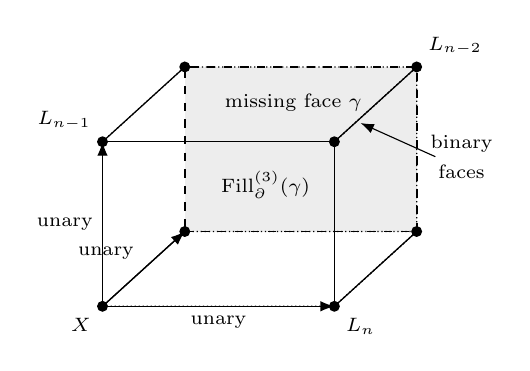
\begin{tikzpicture}[scale=0.95,>=Latex,
  vertex/.style={circle,fill=black,inner sep=1.4pt},
  edge/.style={line width=0.45pt},
  unary/.style={edge,->},
  face/.style={edge,densely dotted},
  missing/.style={edge,dashed,line width=0.7pt}]

\coordinate (x0) at (0,0);
\coordinate (x1) at (3.1,0);
\coordinate (x2) at (0,2.2);
\coordinate (x3) at (3.1,2.2);
\coordinate (y0) at (1.1,1.0);
\coordinate (y1) at (4.2,1.0);
\coordinate (y2) at (1.1,3.2);
\coordinate (y3) at (4.2,3.2);

\fill[gray!14] (y0)--(y1)--(y3)--(y2)--cycle;
\draw[edge] (x0)--(x1)--(x3)--(x2)--cycle;
\draw[edge] (x0)--(y0) (x1)--(y1) (x2)--(y2) (x3)--(y3);
\draw[missing] (y0)--(y1)--(y3)--(y2)--cycle;

\draw[unary] (x0)--node[below] {\scriptsize unary} (x1);
\draw[unary] (x0)--node[left] {\scriptsize unary} (x2);
\draw[unary] (x0)--node[above left] {\scriptsize unary} (y0);

\draw[face] (x1)--(y1)--(y3)--(x3);
\draw[face] (x2)--(y2)--(y3)--(x3);
\draw[face] (x0)--(x1)--(y1)--(y0);

\foreach \p in {x0,x1,x2,x3,y0,y1,y2,y3} \node[vertex] at (\p) {};

\node[below left=1pt of x0] {\scriptsize \(X\)};
\node[below right=1pt of x1] {\scriptsize \(L_n\)};
\node[above left=1pt of x2] {\scriptsize \(L_{n-1}\)};
\node[above right=1pt of y3] {\scriptsize \(L_{n-2}\)};

\node at (2.55,2.72) {\scriptsize missing face \(\gamma\)};
\node at (2.18,1.62) {\scriptsize \(\mathrm{Fill}^{(3)}_{\partial}(\gamma)\)};
\node[align=center] at (4.8,2.0) {\scriptsize binary\\[-1pt]\scriptsize faces};
\draw[->] (4.45,2.0)--(3.45,2.45);
\end{tikzpicture}
\caption{A depth-three structural open box.  Unary action data and already exported binary
comparison faces determine the boundary \(\partial\); the shaded back face is the missing
remote comparison \(\gamma\), and the interior cell is the filler computed by the cubical
operations.}
\label{fig:depth-three-open-box}
\end{figure}

\subsection{Derivedness and minimal public signatures}
\label{subsec:derivedness-minimal-signatures}

The open-box theorem is semantic.  It says that the higher exact factor is contractible.  The
public-signature theorem is syntactic-accounting.  It says that an explicit higher structural
field in a surface presentation can be replaced by the cubically computed term and therefore
removed from the primitive part of a \(\mu\)-minimal signature.

The bridge between the two levels is the computational replacement theorem from
Section~3: when a presented field is accompanied by a uniform derivation from lower public
boundary data, the presentation relation allows the field to be replaced by that derived term.
The open-box theorem supplies exactly such a derivation for higher structural trace.

\begin{thm}[Derived trace witnesses for higher structural horns]
\label{thm:higher-structural-derived-trace}
Let \(h\) be a normalized structural horn package generated by the fixed cubical
sealed-extension grammar, and suppose the historical arity of \(h\) is at least three.  Then
\(h\) carries a derived trace witness in the sense of
Definition~\ref{def:derived-trace-witness}.

Dependencies: syntactic horn reduction, horn-to-open-box adequacy, total open-extension
contractibility, substitution stability, and computational replacement on canonical trace
presentations.
\end{thm}

\begin{proof}
Let \(\partial_h\) be the lower public boundary of \(h\).  By
Lemma~\ref{lem:syntactic-horn-reduction}, the exact additional datum represented by \(h\) is
a dependent sum
\[
  \sum_{\gamma:\Gamma_{\mathrm{miss}}(\partial_h)}
    \mathsf{Fill}_{\partial_h}(\gamma).
\]
By Lemma~\ref{lem:horn-open-box}, this sum is equivalent to the explicit structural
open-box extension decoded from the horn grammar.  The decoded box exposes the family
\(A\), the face formula \(\varphi\), the partial boundary \(u\), the base face \(u_0\), the
compatible lid subtype, and the filler family.

Theorem~\ref{thm:open-ext-contr} gives a canonical center of this open-box extension,
computed by cubical composition and filling.  Transporting that center back along the
horn-to-open-box equivalence gives the replacement term
\[
  t_h(\partial_h)
  :
  \sum_{\gamma:\Gamma_{\mathrm{miss}}(\partial_h)}
    \mathsf{Fill}_{\partial_h}(\gamma).
\]
The typing and boundary equations are the endpoint and side equations of the decoded
open box.  Semantic preservation is the equivalence of
Lemma~\ref{lem:horn-open-box}.  The allowed-dependency condition holds because the decoded
box is assembled from \(\partial_h\) and the fixed cubical operations only.  Substitution
stability is Lemma~\ref{lem:open-box-substitution}.  Finally, public-normalization
compatibility is exactly the hypothesis consumed by the computational replacement theorem of
Section~3: replacing the explicit horn field by the computed center gives a presentation of
the same canonical trace signature in which the horn field is derived rather than primitive.
These are precisely the components required by
Definition~\ref{def:derived-trace-witness}.
\end{proof}

\begin{thm}[Minimal-signature elimination above binary arity]
\label{thm:minimal-signature-elimination}
Let \(e\) be an admissible surface extension declaration over \(B_n\).  Then there exists a
presentation-equivalent declaration \(e'\approx e\) whose normalized trace signature contains
no irreducible primitive historical field of arity \(k\geq 3\).  Equivalently, every canonical
\(\mu\)-minimal normalized public signature contains only unary and binary primitive
structural trace fields.

More concretely, if a presented structural field of arity \(k\geq 3\) occurs in some surface
declaration, then in the canonical trace-presentation interface it is transparently derived
from its lower-arity boundary by a term synthesized from cubical composition, transport, and
filling.

Dependencies: normal-form classification, derived trace witnesses for higher structural
horns, and the computational replacement theorem.
\end{thm}

\begin{proof}
Fix a presentation of \(e\) and an apparent primitive structural trace field \(\phi\) of arity
\(k\geq 3\) in its elaborated sealed export.  By the normal-form classification of Section~4,
\(\phi\) is a higher structural horn package rather than payload.  By
Theorem~\ref{thm:higher-structural-derived-trace}, \(\phi\) carries a
\(\mathsf{DerivedTrace}\) witness.  Concretely, this witness supplies lower boundary data
\(\partial\), the replacement term \(t_\phi(\partial)\), typing and boundary equations,
semantic preservation, allowed-dependency data, substitution stability, and
public-normalization compatibility.

The computational replacement rule of Section~3 then applies: a presented higher structural
field equipped with such a uniform lower-boundary derivation is presentation-equivalent to
the declaration in which the field is replaced by \(t_{\phi}(\partial)\) and classified as
derived by the supplied witness.
Repeating this replacement for every arity-\(k\geq 3\) structural field terminates because the
normalized signature is finite.  The resulting presentation-equivalent declaration \(e'\) has
no primitive structural field above binary arity.  Since \(\mu\) counts only primitive trace
fields in canonical normal form, every \(\mu\)-minimal signature has the same property.
\end{proof}

\begin{defi}[Primitive status and minimal opaque cost]
\label{def:primitive-status-mu}
After the replacement procedure of Theorem~\ref{thm:minimal-signature-elimination}, an atomic
trace schema in a normalized public signature is \emph{derived} if it is synthesized by
transparent normalization, by generic cubical structure, or by a supplied
\(\mathsf{DerivedTrace}\) witness.  It is \emph{primitive} if no such synthesis is available in
the fixed normalization relation.  For an admissible declaration \(e\), let
\(N_{\mathrm{tr}}^{\mathrm{prim}}(e)\) be the resulting primitive trace part.  The minimal
opaque public trace cost is
\[
  \mu(e)
  :=
  \min\{\, |N_{\mathrm{tr}}^{\mathrm{prim}}(e')| \mid e'\approx e \,\}.
\]
This is the formal version of the accounting notation introduced in
Definition~\ref{def:mu-provisional}; in particular, \(\mu\) is attached to canonical
normalized public signatures after witnessed replacement, not to raw declarations.
\end{defi}

\begin{rem}[What is eliminated]
Theorem~\ref{thm:minimal-signature-elimination} eliminates primitive public fields, not exact
semantic factors.  A higher horn factor may still occur in \(\mathrm{Real}_k(X)\), but after
Theorem~\ref{thm:open-ext-contr} it occurs as a contractible factor with a canonical center.
The trace-cost invariant \(\mu\) does not count such a factor as primitive public trace.
\end{rem}

\subsection{Exact stabilization above binary trace}
\label{subsec:exact-stabilization}

We can now prove the upper bound on obligation depth.  The proof is conceptually simple:
from depth two onward, each further exposure of remote history adjoins one structural
open-box extension factor; each such factor is contractible; dependent sums with
contractible fibers are equivalent to their bases.

\begin{lem}[Kan contraction for structural horn fibers]
\label{lem:kan-contraction-horn-fibers}
For every structural horn-extension fiber \(H_k(\partial)\) generated by the fixed cubical
sealing grammar, the projection
\[
  H_k(\partial) \to 1
\]
is contractible in the cubical metatheory.  The center is the missing face and filler computed
from \(\partial\) by the cubical operations.

Dependencies: horn-to-open-box adequacy and total open-extension contractibility.
\end{lem}

\begin{proof}
By Lemma~\ref{lem:horn-open-box}, \(H_k(\partial)\) is the open-box extension type for the
structural tuple \((A_k,\varphi_k,u_k,u^0_k)\).  Applying
Theorem~\ref{thm:open-ext-contr} gives a canonical center and a contraction of the whole
extension space.  Presentation equivalence is not used to prove this contractibility; it is
used only in Theorem~\ref{thm:minimal-signature-elimination} to classify the corresponding
public field as derived.
\end{proof}

\begin{thm}[Exact stabilization of realized structural obligations]
\label{thm:exact-stabilization}
In the fixed cubical extension calculus, for every foundational-core candidate \(X\) and
every \(k\geq 2\) there is a canonical equivalence
\[
  \mathrm{Real}_k(X) \simeq \mathrm{Real}_2(X).
\]
Consequently \(d_{\mathrm{obl}}\leq 2\).

Dependencies: the formal definition of \(\mathrm{Real}_k\), arity-cell identification,
syntactic horn reduction, horn-to-open-box adequacy, and total open-extension
contractibility.
\end{thm}

\begin{proof}
The case \(k=2\) is immediate.  For \(k=3\), Lemmas~\ref{lem:arity-cell} and
\ref{lem:syntactic-horn-reduction} identify the marginal depth-three datum over each
boundary \(\partial:\mathrm{Real}_2(X)\) as the horn-extension fiber \(H_3(\partial)\).  Hence
\[
  \mathrm{Real}_3(X)
  \simeq
  \sum_{\partial:\mathrm{Real}_2(X)} H_3(\partial).
\]
By Lemma~\ref{lem:kan-contraction-horn-fibers}, every fiber \(H_3(\partial)\) is
contractible.  A dependent sum over a family of contractible fibers is canonically equivalent
to its base, so
\[
  \mathrm{Real}_3(X) \simeq \mathrm{Real}_2(X).
\]

For \(k>3\), the same argument repeats.  Passing from depth \(k-1\) to depth \(k\) exposes
one additional remote layer and adjoins one structural horn-extension fiber \(H_k(\partial)\)
over \(\partial:\mathrm{Real}_{k-1}(X)\).  Lemma~\ref{lem:kan-contraction-horn-fibers}
contracts that fiber, so
\[
  \mathrm{Real}_k(X) \simeq \mathrm{Real}_{k-1}(X)
  \qquad (k\geq 3).
\]
Iterating these equivalences yields \(\mathrm{Real}_k(X)\simeq\mathrm{Real}_2(X)\) for all
\(k\geq 2\).
\end{proof}

\begin{cor}[Contractible-factor decomposition]
\label{cor:contractible-factor-decomposition}
For every foundational-core candidate \(X\) and every \(k\geq 2\), there is a canonical
equivalence
\[
  \mathrm{Real}_k(X)
  \simeq
  \mathrm{Real}_2(X) \times C_k(X),
\]
where \(C_2(X):=1\) and, for \(k>2\), \(C_k(X)\) is the iterated chain of canonical remote
horn factors selected by the cubical compositions in the proof of
Theorem~\ref{thm:exact-stabilization}.  Each \(C_k(X)\) is canonically contractible.

Dependencies: exact stabilization and Kan contraction for structural horn fibers.
\end{cor}

\begin{proof}
The proof of Theorem~\ref{thm:exact-stabilization} trivializes each successive horn-extension
fiber by choosing its canonical cubical center.  Iterating those choices identifies the total
higher part with a product of the depth-two boundary and the chain of chosen remote horn
factors.  Each factor is contractible by Lemma~\ref{lem:kan-contraction-horn-fibers}, hence
the whole chain \(C_k(X)\) is contractible.
\end{proof}

The corollary expresses the exact semantic situation more vividly than the bare equivalence:
above depth two there may be additional exact factors, but all of them are canonical and
contractible.  The primitive public signature sees only the depth-two part.

\subsection{From arity depth to a two-layer chronological window}
\label{subsec:recent-history}

The exact-depth theorem bounds arity.  It does not, by itself, identify which layers must be
inspected in time.  A primitive binary field could still compare a new layer with a remote
old layer.  The next theorem rules out such primitive remote binary fields for the fixed
calculus, using the factorization-complete public exports introduced earlier.

\begin{thm}[Recent-history factorization]
\label{thm:recent-history-factorization}
In the fixed cubical extension calculus, every binary trace field that survives in a
\(\mu\)-minimal normalized public signature at stage \(n+1\) factors through the previous two
normalized signatures.  More precisely, let \(X\) be sealed at stage \(n+1\).  Once the unary
and binary trace data of \(X\) against \(L_n\) and \(L_{n-1}\) have been fixed, every
comparison between \(X\) and a remote layer \(L_{n-r}\), for \(r\geq 2\), is
definitionally equal after normalization to a term obtained by iterating the already exported
unary bridges and binary comparison traces of the intervening normalized signatures.
Consequently no \(\mu\)-minimal public signature contains a primitive remote binary field.

Dependencies: factorization-complete export, the normal-form classification of structural
trace, minimal-signature elimination, and the preceding exact stabilization theorem.
\end{thm}

\begin{proof}
Consider first the layer \(L_{n-2}\).  The sealed export of \(L_n\) contains the adjacent
unary bridge to \(L_{n-1}\), and the sealed export of \(L_{n-1}\) contains the adjacent bridge
to \(L_{n-2}\).  The binary part of the trace exported by these layers records the comparison
between the adjacent composite and the corresponding direct public route.  Since exports are
factorization-complete, the degenerate faces and transport faces needed to assemble the next
comparison box are transparent public data.

When \(X\) is sealed against \(L_n\) and \(L_{n-1}\), it supplies the unary comparisons to
those two layers and the binary square comparing the two routes through them.  Combining
this data with the exported adjacent bridges determines all visible faces of an open
three-box.  The missing face is exactly the would-be direct comparison from \(X\) to
\(L_{n-2}\).  Thus the remote comparison is not an independent primitive binary field; it is
the lid of a structural horn-extension object.  Cubical composition computes that lid, and
cubical filling supplies the accompanying three-cell.  By Theorem~\ref{thm:minimal-signature-elimination},
the presented remote comparison is therefore replaced by the derived term in every
\(\mu\)-minimal signature.

The argument iterates.  Suppose the comparison from \(X\) to \(L_{n-r+1}\) has already
been factored through recent exported signatures.  The normalized export of \(L_{n-r+1}\)
contains the adjacent bridge to \(L_{n-r}\), the binary comparison trace for the composite
through that bridge, and the transparent degenerate faces needed for the next open box.
Combining these with the already factored comparison for \(X\) produces another structural
horn-extension problem whose missing face is the comparison from \(X\) to \(L_{n-r}\).
Cubical composition and filling synthesize that face and filler.  Hence every remote binary
comparison is definitionally generated from the recent public exports and is not primitive in
canonical minimal form.
\end{proof}

\begin{cor}[Two-layer chronological window]
\label{cor:two-layer-window}
In the fixed cubical extension calculus, every sealing step at stage \(n+1\) has chronological
window size at most two.  All primitive obligations are generated by the exported traces of
\(L_n\) and \(L_{n-1}\), while comparisons with layers \(L_{n-r}\) for \(r\geq 2\) factor
through those two normalized signatures and are synthesized by iterated cubical filling.

Dependencies: exact stabilization and recent-history factorization.
\end{cor}

\begin{proof}
Theorem~\ref{thm:exact-stabilization} shows exact arity stabilization at depth two, while
Theorem~\ref{thm:recent-history-factorization} shows that surviving binary primitive fields
can be chosen to factor through the two most recent normalized signatures.  Therefore deeper
history contributes only derived fillers and already mediated boundary data, not primitive
public trace fields outside the recent two-layer window.
\end{proof}

The recurrence theorem in Section~6 starts only after this point.  It counts the active basis
inside the two-layer chronological window under an additional full-coupling hypothesis.

\subsection{The lower bound: univalence forces binary trace}
\label{subsec:swap-lower-bound}

It remains to show that the upper bound is exact.  The obstruction is small but decisive.
A univalent interface that exports the two-point type also exports the path corresponding to
its nontrivial automorphism.  A sealed action must respect that path.  Objectwise unary data
alone cannot express this naturality condition.

\begin{thm}[Explicit binary sealing obstruction]
\label{thm:swap-obstruction}
Let the active interface of a univalent foundation export the two-point type \(2\) and the
univalent path
\[
  p_{\mathrm{swap}} := \mathrm{ua}(\mathrm{swap}) : 2 = 2.
\]
Then there exists an objectwise promoted-interface candidate whose unary clause is
well-formed on the active object \(2\), while the corresponding binary sealing obligation over
\(p_{\mathrm{swap}}\) is uninhabited.  Equivalently, the unary fragment admits a raw
objectwise action that the binary fragment rejects.  Consequently depth-one data are
insufficient in general, and \(d_{\mathrm{obl}}\geq 2\).

Dependencies: the univalent two-point interface, transport in the endomorphism family, and
the distinction between unary objectwise action and binary sealing naturality.
\end{thm}

\begin{proof}
Consider an active-interface package consisting of an endomap on the exported two-point
type:
\[
  X_{\mathrm{act}} := (F_2 : 2\to 2).
\]
The unary candidate chooses the constant-left map
\[
  F_2 := \lambda\_.\,\mathsf{left}.
\]
This is a well-formed objectwise clause.  But sealing a globally acting structural extension
requires compatibility with exported paths.  Since the interface exports
\(p_{\mathrm{swap}}\), the binary naturality obligation is
\[
  \alpha_{\mathrm{swap}}:
  \mathrm{transport}_{\lambda A. A\to A}(p_{\mathrm{swap}},F_2)=F_2.
\]
By univalence, transport in the endomorphism family along \(p_{\mathrm{swap}}\) computes by
conjugation with the swap equivalence.  Therefore
\[
  \mathrm{transport}_{\lambda A. A\to A}(p_{\mathrm{swap}},F_2)
  =
  \mathrm{swap}\circ F_2\circ \mathrm{swap}^{-1}
  =
  \lambda\_.\,\mathsf{right}.
\]
Thus \(\alpha_{\mathrm{swap}}\) would be an equality
\[
  (\lambda\_.\,\mathsf{right})=(\lambda\_.\,\mathsf{left}),
\]
which is impossible because evaluating at \(\mathsf{left}\) would force
\(\mathsf{right}=\mathsf{left}\).

There is also a positive control: if \(F_2\) is the identity map, conjugation along swap
returns the identity map, and the binary obligation is inhabited.  The failure of the
constant-left map is therefore not a defect of the formulation; it is the type checker
detecting an objectwise action that does not respect exported path structure.  Hence
there is a unary-accepted raw action whose binary sealing extension is impossible.  In
particular, \(\mathrm{Real}_1\) can be inhabited in a case where the corresponding
\(\mathrm{Real}_2\) fiber is empty, so \(\mathrm{Real}_1\) and \(\mathrm{Real}_2\) are not
canonically equivalent in general.  The obligation depth cannot be one.
\end{proof}

\begin{rem}[Adjunctions as an explanatory analogue]
Adjunctions exhibit the same binary pattern categorically.  Once the object action and the
unit/counit data have been fixed, the triangle identities compare composites already
determined at the unary level.  The paper uses this only as an analogy.  The internal lower
bound for the fixed cubical calculus is the swap obstruction of
Theorem~\ref{thm:swap-obstruction}.
\end{rem}

\subsection{Exact public structural depth two}
\label{subsec:exact-depth-two-conclusion}

We can now combine the upper and lower bounds.

\begin{cor}[Fixed-calculus exact structural integration depth two]
\label{cor:exact-depth-two}
In the fixed cubical sealed-extension calculus, admissible sealed structural extensions have
exact structural integration depth two:
\[
  d_{\mathrm{obl}}=2.
\]
Moreover every \(\mu\)-minimal normalized public signature contains no primitive structural
trace field of historical arity greater than two, and every sealing step has a two-layer
chronological window under the factorization-complete export hypothesis.

Dependencies: exact stabilization for the upper bound, minimal-signature elimination for
the public-signature statement, recent-history factorization for the chronological window,
and the swap obstruction for the lower bound.
\end{cor}

\begin{proof}
Theorem~\ref{thm:exact-stabilization} gives the upper bound
\(d_{\mathrm{obl}}\leq 2\) by showing
\(\mathrm{Real}_k(X)\simeq\mathrm{Real}_2(X)\) for all \(k\geq 2\).  Theorem~\ref{thm:minimal-signature-elimination}
turns the same cubical horn computation into the public-signature statement
\(d_\mu\leq 2\).  Theorem~\ref{thm:recent-history-factorization} and
Corollary~\ref{cor:two-layer-window} give the separate chronological factorization needed
for the later recurrence.  Finally, Theorem~\ref{thm:swap-obstruction} gives the lower bound
\(d_{\mathrm{obl}}\geq 2\) by exhibiting a genuine binary sealing obstruction in the univalent
setting.  Hence the exact obligation depth is two.
\end{proof}

The result should be read with the distinctions of Remark~\ref{rem:five-statuses} in mind.
Higher structural exact factors do not vanish from the semantics; they stabilize as
contractible open-box extension factors.  What disappears from the primitive public
interface is the need to present those factors as irreducible fields.  This is the semantic
content behind the paper's slogan:
\[
  \text{binary trace is necessary; higher structural trace is cubically payable.}
\]

\section{Counting consequences}
\label{sec:scaling}

The preceding section proves the semantic depth theorem for the fixed cubical
sealed-extension calculus.  This section keeps only the accounting consequence needed in the
main paper: once a two-layer chronological window and full active-basis coupling are imposed,
primitive public trace satisfies an affine recurrence.

The answer is intentionally conditional.  The recurrence below is not a law of ordinary
library growth.  It is the arithmetic shadow of three prior choices:
\begin{enumerate}
\item a genuine chronological window has already been identified;
\item a new sealed layer is advertised as globally acting on the active interface in that
window; and
\item the bundled per-site convention is used, so one active primitive basis site contributes
one primitive public interaction schema for the whole payload package.
\end{enumerate}
Without these assumptions, one gets only a sparse footprint formula.  A local datatype, a
transparent helper definition, or an orthogonal library construction may touch only a few
active sites, or none at all.  Such declarations are not expected to satisfy a Fibonacci law.

A useful way to read the section is:
\[
  \text{depth theorem}
  \quad+\quad
  \text{chronological factorization}
  \quad+\quad
  \text{full coupling}
  \quad\Longrightarrow\quad
  \text{affine recurrence}.
\]
The Fibonacci statement is retained only as the constant-payload endpoint of this recurrence.
Sparse variants, wrapper examples, and refactoring robustness belong in the artifact
documentation rather than in the main proof line.

\subsection{Layerwise quantities and the active window}
\label{subsec:layerwise-quantities}

We begin by naming the quantities that enter the count.  All of them are computed after
normalization.  In particular, a different record packaging, a different bracketing of a
Sigma-telescope, or an explicit surface field that is later replaced by a cubical horn term
does not change the numbers below.

\begin{defi}[Layerwise payload, trace, and basis size]
\label{def:layerwise-payload-trace}
Let
\[
  e_n
\]
be the admissible surface declaration whose sealing exports the stage-
\(n\) layer \(L_n\), and let \(X_n := X(e_n)\) be its elaborated candidate in the raw calculus.
The \emph{payload contribution} of layer \(n\) is
\[
  \kappa_n := \kappa(X_n) := |S_{\mathrm{core}}(L_n)|.
\]
The \emph{primitive trace contribution} of layer \(n\) is
\[
  \mu_n := \mu(e_n) := |S_{\mathrm{str}}(L_n)|.
\]
The normalized active basis exported by the layer is the disjoint union of its payload and
primitive trace basis:
\[
  S_{\mathrm{bas}}(L_n)
  := S_{\mathrm{core}}(L_n) \sqcup S_{\mathrm{str}}(L_n),
\]
and hence
\[
  |S_{\mathrm{bas}}(L_n)| = \kappa_n + \mu_n.
\]
\end{defi}

The notation \(S_{\mathrm{bas}}(L_n)\) is deliberately basis-level notation.  It does not count
all textual declarations exported by a layer.  It counts irreducible active primitive sites
after opacity, normalization, and derived-field elimination.  If a large bundle is treated as
one active basis site by the chosen convention, then it contributes one site.  If the bundle is
split into several independent active sites in the counting normal form, then it contributes
several.  This is why the recurrence is a theorem about normalized public signatures rather
than source files.

\begin{defi}[Depth-\(d\) historical basis window]
\label{def:historical-basis-window}
Assume that a foundation or extension discipline has a chronological window of size \(d\).
At stage \(n+1\), the depth-\(d\) active historical basis is the tagged coproduct
\[
  I^{(d)}_{n,\mathrm{bas}}
  :=
  \coprod_{j=0}^{d-1} S_{\mathrm{bas}}(L_{n-j}).
\]
For bootstrap stages, where some layer \(L_{n-j}\) does not yet exist, the corresponding
summand is defined to be the empty basis.
\end{defi}

The tags matter.  The same primitive shape appearing in two different sealed layers is counted
as two historical basis sites, because a new globally acting layer must specify how it
interacts with each opaque export as an export.  Conversely, two syntactic names in one layer
that normalize to the same active basis site are counted once.

\begin{rem}[Indexing convention]
\label{rem:scaling-indexing}
The layer \(L_n\) is exported by the declaration \(e_n\).  Its payload contribution is
\(\kappa_n\), its primitive public trace contribution is \(\mu_n\), and its normalized active
basis size is \(\kappa_n+\mu_n\).  The declaration exporting \(L_{n+1}\) is counted against
the active window ending at \(L_n\).  Thus, in the depth-two cubical case, the recurrence for
\(\mu_{n+1}\) uses \(L_n\) and \(L_{n-1}\):
\[
  \mu_{n+1}
  = \mu_n + \mu_{n-1} + \kappa_n + \kappa_{n-1}.
\]
This equality is asserted after the two-layer window has been populated.  Earlier bootstrap
steps use the empty-interface convention from Definition~\ref{def:historical-basis-window}.
\end{rem}

The next distinction is the one that prevents the recurrence theorem from being read too
broadly.

\begin{defi}[Sparse footprint and full coupling]
\label{def:sparse-footprint-full-coupling}
A stage-\(n+1\) declaration has a \emph{sparse active footprint} of depth \(d\) if it selects a
finite sub-basis
\[
  \mathrm{Foot}^{(d)}_n \subseteq I^{(d)}_{n,\mathrm{bas}}
\]
of the historical basis window.  Its sparse trace cost is the size of that selected footprint.

The declaration is \emph{fully coupled} against the depth-\(d\) window when
\[
  \mathrm{Foot}^{(d)}_{n,\mathrm{full}} = I^{(d)}_{n,\mathrm{bas}}.
\]
In words: the new sealed layer is advertised as globally acting on every active primitive basis
site in the relevant public window.
\end{defi}

Sparse footprints are the default for ordinary extension.  A definition may use only the
list type, only one universe level, or only a small set of operations.  Full coupling is a
special foundational-core regime.  A modality, universe-level operation, or promoted structural
package may advertise an action on the entire active interface.  The recurrence theorem is
about this special endpoint.

\subsection{Sparse footprints before the full envelope}
\label{subsec:sparse-footprints}

The arithmetic begins with a finite-set decomposition.  Since the historical window is a
tagged coproduct of layer bases, any selected footprint decomposes uniquely into the part it
selects from each recent layer.

\begin{lem}[Window cardinality]
\label{lem:window-cardinality}
Let a stage-\(n+1\) declaration use an active footprint
\[
  \mathrm{Foot}^{(d)}_n \subseteq I^{(d)}_{n,\mathrm{bas}}.
\]
Then
\[
  |\mathrm{Foot}^{(d)}_n|
  =
  \sum_{j=0}^{d-1}
  \bigl|\mathrm{Foot}^{(d)}_n \cap S_{\mathrm{bas}}(L_{n-j})\bigr|.
\]
If the declaration is fully coupled, then
\[
  |\mathrm{Foot}^{(d)}_{n,\mathrm{full}}|
  =
  \sum_{j=0}^{d-1}
  (\kappa_{n-j}+\mu_{n-j}).
\]

Dependencies: tagged-coproduct decomposition of the historical window and the layerwise
payload/primitive-trace basis identity.
\end{lem}

The proof is finite-set bookkeeping.  A finite subset of the tagged coproduct
\(I^{(d)}_{n,\mathrm{bas}}=\coprod_{j=0}^{d-1}S_{\mathrm{bas}}(L_{n-j})\) is the disjoint union
of its intersections with the tagged summands.  In the fully coupled case, each intersection is
the entire summand, and Definition~\ref{def:layerwise-payload-trace} identifies the summand
size with \(\kappa_{n-j}+\mu_{n-j}\).  Sparse footprints give the first displayed formula but
not the full-coupling recurrence.

\subsection{The full-coupling affine recurrence}
\label{subsec:full-coupling-recurrence}

We can now state the general recurrence.  It is parameterized by a chronological window size
\(d\).  In the fixed cubical calculus, Section~5 supplies \(d=2\).  In a UIP-like collapse,
one may have \(d=1\).  Other window sizes are included only to make clear which part of the
proof is arithmetic and which part is semantic.

\begin{thm}[Full-coupling affine recurrence under a depth-\(d\) window]
\label{thm:full-coupling-affine-recurrence}
Let a sealed extension discipline have obligation depth realized by a chronological window of
size \(d\).  Assume that the stage-\(n+1\) declaration is fully coupled against the whole
active window:
\[
  \mathrm{Foot}^{(d)}_{n,\mathrm{full}} = I^{(d)}_{n,\mathrm{bas}}.
\]
Then the primitive trace cost of the next sealed layer satisfies
\[
  \mu_{n+1}
  =
  \sum_{j=0}^{d-1} (\mu_{n-j}+\kappa_{n-j})
  \qquad (n\geq d),
\]
with bootstrap stages interpreted using empty earlier layers.

Dependencies: window cardinality, the trace-cost dictionary, and the full-coupling footprint
hypothesis.
\end{thm}

\begin{proof}
By the trace-cost dictionary, the minimal opaque cost of the next sealed layer is the size of
its active primitive footprint:
\[
  \mu_{n+1}=|\mathrm{Foot}^{(d)}_{n,\mathrm{full}}|.
\]
Full coupling identifies this footprint with the whole historical basis window.  Lemma~\ref{lem:window-cardinality} gives
\[
  |\mathrm{Foot}^{(d)}_{n,\mathrm{full}}|
  =
  \sum_{j=0}^{d-1} (\kappa_{n-j}+\mu_{n-j}).
\]
Substitution yields the displayed recurrence.
\end{proof}

The theorem is deliberately modest.  It does not prove that a system has window size \(d\),
and it does not prove that a declaration is fully coupled.  Those are semantic and
presentation-level hypotheses.  The theorem says that once those hypotheses are supplied, the
trace count is forced.

\begin{cor}[Depth-two full-coupling recurrence in the fixed calculus]
\label{cor:depth-two-full-coupling-recurrence}
In the fixed fully coupled cubical sealed-extension calculus, the two-layer chronological
factorization theorem of Section~5 gives
\[
  \mu_{n+1}
  =
  \mu_n+\mu_{n-1}+\kappa_n+\kappa_{n-1}
  \qquad (n\geq 2).
\]

Dependencies: recent-history factorization and the full-coupling affine recurrence.
\end{cor}

This is Theorem~\ref{thm:full-coupling-affine-recurrence} with \(d=2\), using the
recent-history factorization theorem to identify the primitive public-support window of the
fixed cubical calculus.

Let
\[
  \tau_n := \sum_{i=1}^{n}\mu_i
\]
be the cumulative minimal opaque trace cost through stage \(n\).  This cumulative quantity is
not used in the semantic depth theorem; it is useful only for comparing growth rates across
window sizes.

\subsection{The depth-two Fibonacci endpoint}
\label{subsec:fibonacci-endpoint}

We now specialize the depth-two recurrence to constant payload size.  This is the place where
Fibonacci growth appears.  It should be read strictly as an asymptotic theoretical
worst-case envelope: the endpoint of full coupling, uniform payload size, bundled per-site
counting, and the empty-history bootstrap, not as the definition of coherence depth two.

Let \((F_n)_{n\geq 1}\) be the Fibonacci sequence with
\[
  F_1=F_2=1,
  \qquad
  F_{n+1}=F_n+F_{n-1}.
\]

\begin{cor}[Constant-payload full-coupling Fibonacci endpoint]
\label{cor:affine-fibonacci-envelope}
In the fixed fully coupled cubical sealed-extension calculus, assume obligation depth two is
realized by the two-layer chronological window and every sealed layer contributes the same
core payload size \(c\).  Then
\[
  \mu_{n+1}=\mu_n+\mu_{n-1}+2c.
\]
Define the shifted sequence
\[
  U_n := \mu_n+2c.
\]
Then
\[
  U_{n+1}=U_n+U_{n-1}.
\]
If the initial state exports no prior sealed layers, then
\[
  \mu_1=0,
  \qquad
  \mu_2=c,
\]
and consequently
\[
  U_n=cF_{n+2},
  \qquad
  \mu_n=c(F_{n+2}-2),
\]
while the cumulative minimal opaque cost satisfies
\[
  \tau_n=c(F_{n+4}-2n-3).
\]

Dependencies: the depth-two full-coupling recurrence, the uniform-payload assumption, and
the empty-history bootstrap convention.
\end{cor}

\begin{proof}
Corollary~\ref{cor:depth-two-full-coupling-recurrence} gives
\[
  \mu_{n+1}
  =
  \mu_n+\mu_{n-1}+\kappa_n+\kappa_{n-1}.
\]
Under the uniform-payload assumption \(\kappa_n=c\), this becomes
\[
  \mu_{n+1}=\mu_n+\mu_{n-1}+2c.
\]
Adding \(2c\) to both sides yields
\[
  \mu_{n+1}+2c
  =
  (\mu_n+2c)+(\mu_{n-1}+2c),
\]
which is exactly \(U_{n+1}=U_n+U_{n-1}\).

For the bootstrap values, the first layer sees no previous sealed public interface, so
\(\mu_1=0\).  The second layer sees only the first layer's payload basis, of size \(c\), and
therefore \(\mu_2=c\).  Hence
\[
  U_1=2c=cF_3,
  \qquad
  U_2=3c=cF_4.
\]
Since \((U_n)\) and \((cF_{n+2})\) satisfy the same recurrence and agree at the first two
stages, induction gives \(U_n=cF_{n+2}\).  Subtracting \(2c\) gives the formula for
\(\mu_n\).  Finally,
\[
  \tau_n
  =
  \sum_{i=1}^{n} c(F_{i+2}-2)
  =
  c(F_{n+4}-2n-3),
\]
using the standard identity \(\sum_{i=1}^n F_{i+2}=F_{n+4}-3\).
\end{proof}

This endpoint is only the constant-payload full-coupling specialization.  Sparse footprints and
alternative wrapper disciplines are supported by the artifact documentation, but they are not
needed in the main text.

\section{Mechanization, transfer, and trusted boundary}
\label{sec:mechanization}

The accompanying Cubical Agda development is a theorem-facing artifact for the fixed calculus
studied in this paper.  It is available at
\url{https://github.com/efficient-novelty/coherence-depth}; this GitHub repository is the
development location and reproducibility target.  A citable Zenodo archive with a DOI is still
required before LMCS submission, so the GitHub URL should not be read as the final archival
citation.  The detailed artifact map and reproducibility instructions are collected in
Appendix~\ref{app:mechanization-audit}.  The
development is not used as a substitute for the mathematical argument; it checks the proof
stack at the places where informal prose is most likely to hide a boundary, especially the
distinction between classifying a structural field as derived and replacing it by cubical
composition and filling.  Broader transfer remains routed through the adequacy interface of
Section~3.

\subsection{The checked proof stack}
\label{subsec:mechanization-checked-stack}

The formalization follows the same layers as the paper, but each layer has its own status.  The
raw calculus represents payload, trace roles, historical support, normalized public signatures,
and \(\mu\) for the encoded fixed calculus.  The cubical core checks the theorem-facing
open-box package used by the artifact, using Cubical Agda partial elements, \texttt{hcomp},
\texttt{hfill}, and reindexing data; when the paper asks for a fuller
path-through-compatible-elements adequacy reading, that reading is recorded as an adequacy
boundary rather than silently folded into the theorem.  The horn layer checks
constructor-by-constructor decoding for the sealing-generated higher horn grammar.  The replacement layer
checks canonical trace presentations for the encoded interfaces.  The lower-bound layer checks
the two-point swap obstruction, the exact-depth layer checks the depth-two and chronological-
window wrappers in the recorded scope, and the counting layer checks the sparse footprint law,
the full-coupling affine recurrence, and the constant-payload Fibonacci specialization under
the listed hypotheses.

The development also contains the concrete SMod surface adequacy instance used as the running
example: it preserves payload, primitive trace, derived horn trace, historical support, and
public trace cost.

\begin{thm}[Mechanized theorem stack, paper reading]
\label{thm:mechanized-theorem-stack}
Relative to the trusted cubical base and the fixed definitions of \(C_{\mathrm{ext}}\), the
Agda development provides the following status-classified support:
\begin{enumerate}
\item fully mechanized checks for the encoded raw-calculus discipline, canonical trace
presentations, presentation equivalence, \(\mu\)-invariance, the SMod adequacy instance,
concrete lower-bound witnesses, exact-depth wrappers for the fixed package, arithmetic
recurrences, refactoring invariance, and audit fixtures;
\item mechanization for abstract interfaces for theorem-facing open-box, horn-computation,
semantic-wrapper, chronological-window, and 2D-foundation packages whose record
hypotheses are supplied explicitly;
\item conditional-on-adequacy support for claims that pass from a surface language, broad
semantic foundation, or paper-level \(\mu\)-reading through \texttt{RawAdequacyPackage}; many
of these rows are checked Agda theorems internally, but their external semantic reading still
requires the named adequacy bridge;
\item paper-only support where the prose uses a broader reading than the checked record, such
as basis-choice explanations or final archival-citation requirements.
\end{enumerate}
\end{thm}

\begin{proof}[Artifact proof reading]
Each checked item is represented by the theorem-facing modules summarized in
Appendix~\ref{app:mechanization-audit}.  The aggregate script checks the import closure
containing those modules, the paper-map checker verifies that the paper labels and listed Agda
theorem names exist, and the postulate audit reports no local postulates or local primitive
declarations inside the theorem-facing closure.  The conclusion is therefore deliberately
status-indexed: a fully mechanized row is a theorem of the encoded artifact, an
abstract-interface row is a theorem of the displayed record assumptions, a conditional row
supports the intended external reading only after the named adequacy package or bridge is
supplied, and a paper-only row is not claimed as checked.
\end{proof}

\subsection{Trusted boundary}
\label{subsec:mechanization-trusted-boundary}

The trusted base is small but not empty.  It consists of the Agda kernel running with cubical
support and safety options, the pinned Cubical Agda library declared by the artifact files, the
fixed raw extension-calculus specification used as the theorem object, and the small arithmetic
layer used by the counting proofs.  Optional case-study fixtures may import additional Cubical
library interfaces, but they are not premises of the main theorem.

The absence of local postulates is an audit result about the theorem-facing closure.  It means
that the local modules used by the theorem map typecheck without local \texttt{postulate}
declarations or local Agda \texttt{primitive} declarations beyond the trusted cubical primitives
imported from the selected library.  It is not, by itself, an adequacy theorem for every external
foundation.

The \texttt{RawAdequacyPackage} is an assumed interface in broad semantic wrappers and a
concrete checked instance for the selected raw and SMod fragments.

\subsection{What remains outside}
\label{subsec:outside-mechanized-claim}

The artifact boundary has five parts: broad transfer still needs the adequacy interface; there
is no parser or elaborator theorem for arbitrary Cubical Agda source programs; contractibility
is proved for structural open-box extension fibers, not arbitrary higher filler spaces; the
recurrence applies only under its two-layer-window and full-coupling hypotheses; and the Agda
kernel, Cubical library interface, stated imports, and visible
\texttt{UnsupportedIndexedMatch} warning class remain part of the trusted and audited
boundary.

\subsection{Summary}
\label{subsec:mechanization-summary}

The mechanization supports the main message of the paper in a status-indexed sense.  For the
encoded fixed calculus \(C_{\mathrm{ext}}\), it checks the raw-calculus and trace-presentation
components, structural horn decoding, theorem-facing open-box abstractions, computational
replacement, exact-depth and chronological-window wrappers in the recorded scope, the binary
lower bound supplied by the swap obstruction, and the counting consequences under
recent-history and full-coupling hypotheses.  Where the paper reads these records as external
semantic claims, the result is conditional on the corresponding adequacy package.

The formalization therefore strengthens the paper's central claim, but it does not erase the
semantic boundary.  The fixed theorem is checked.  The SMod bridge is checked as a representative
adequacy instance.  The broad claim that many other cubical foundations or surface languages
instantiate the same interface remains a transfer program: plausible, sharply specified, and
not assumed by the main theorem.  Appendix~\ref{app:mechanization-audit} records the detailed
artifact map, status vocabulary, fixture audit, and recommended reading path.

\section{Conclusion}
\label{sec:conclusion}

This paper began with a simple question about foundational growth.  When a cubical
foundation is extended by a sealed, globally acting structural layer, how much of the
resulting integration burden must remain as primitive public data?  A sealed extension is
not merely another transparent definition in a library.  It exports an interface, and that
interface must explain how the new layer acts on the active structure that the old foundation
already exposes.  The explanatory residue is public trace.

The main result is that, in the fixed sealed-extension calculus studied here, this public
structural trace has exact depth two.  Unary action trace is not enough: univalence makes
binary comparison data public, and a sealed action must respect it.  But higher
sealing-generated structural trace is not primitive.  Once the unary and binary boundary data
are present, the remaining structural obligations are open-box extension problems.  Cubical
composition, filling, and transport compute the missing faces and fillers.  Thus the exact
semantic obligation object still contains higher factors, but those factors are contractible;
the normalized opaque public signature contains no primitive structural trace fields above
binary arity.

In slogan form:
\begin{quote}
Binary trace is necessary; higher structural trace is cubically payable.
\end{quote}

This conclusion is intentionally stated for the fixed calculus \(C_{\mathrm{ext}}\).  The
calculus is not a decorative presentation of an already obvious fact.  It is the theorem
object.  Its definitions separate payload from trace, primitive fields from derived
horn-computational fields, exact realized obligations from \(\mu\)-minimal public signatures,
and arity depth from chronological support.  Those separations are what make the depth-two
claim precise.

\subsection{The theorem stack}
\label{subsec:conclusion-theorem-stack}

The proof proceeds through a stack of results, each doing a different kind of work.

First, the raw calculus gives a disciplined account of public trace.  A sealed declaration has
payload, unary action trace, binary comparison trace, and higher structural horn packages.
Only the first two trace roles are candidates for primitive structural integration cost in a
minimal public signature.  Higher structural packages are retained in the exact obligation
object, but they are recorded as theorem-facing obligations whose derivedness must be justified
by cubical computation.

Second, the adequacy and normalization layer explains why the paper does not count surface
syntax directly.  Surface presentations may include redundant fields, explicit higher
coherence witnesses, or alternative notations for the same public behavior.  The trace cost
\(\mu\) is attached to normalized opaque signatures, not to arbitrary presentations.  The SMod
instance shows that this boundary is non-vacuous: a concrete surface fragment can elaborate
into the raw calculus while preserving payload, public trace, historical support, and
primitive-versus-derived status.

Third, the structural horn layer identifies the exact shape of the higher obligations.  The
important theorem is not a closed-boundary uniqueness theorem for arbitrary higher homotopy.
It is an open-box theorem for the marginal structural extension problems generated by sealing.
The lower-dimensional faces come from already exported unary and binary trace; the missing
face and interior filler are computed by the cubical Kan operations.  This is the point at
which cubicality does real work.

Fourth, the computational replacement theorem turns semantic fillability into public-trace
elimination.  If a presentation contains an explicit higher structural field, the normalizer
replaces it by a cubical term synthesized from its boundary data.  After this replacement the
field is absent from the \(\mu\)-minimal primitive signature.  This is the reason that
``derived'' is not merely a syntactic label in the intended theorem: it is backed by a
replacement operation and a public-cost invariance statement.

Fifth, the exact depth theorem combines the cubical upper bound with the univalent lower
bound.  The upper bound says that all structural obligations of arity greater than two are
contractible over the binary boundary and therefore primitive-publicly eliminable.  The lower
bound uses the two-point swap obstruction: unary action data alone cannot in general decide
whether a sealed action respects the public comparison induced by a nontrivial equivalence.
Together these results give exact structural integration depth two for \(C_{\mathrm{ext}}\):
\[
  \mathsf{Real}_k(X) \simeq \mathsf{Real}_2(X)
  \qquad (k \geq 2),
\]
while depth one fails in general.

Finally, the counting theorems show what happens after the semantic depth theorem is combined
with additional locality and coverage hypotheses.  Depth as arity does not by itself imply a
chronological recurrence: a binary comparison can still refer to remote history.  The
recent-history theorem adds a factorization-complete export condition under which remote
comparisons factor through the two most recent normalized signatures.  Full coupling then
turns the semantic window into arithmetic:
\[
  \mu_{n+1}
  =
  \mu_n + \mu_{n-1} + \kappa_n + \kappa_{n-1}.
\]
The Fibonacci endpoint is the constant-payload specialization of this recurrence, not the
central theorem of the paper.

\subsection{What the result does not say}
\label{subsec:conclusion-nonclaims}

Several nonclaims are as important as the theorem itself.

The result does not say that higher paths disappear from cubical type theory.  Cubical
foundations are rich precisely because higher structure is available and computationally
meaningful.  The theorem concerns the primitive public trace forced by sealing a globally
acting structural extension.  User-supplied higher payload, internal higher homotopy, and
ordinary higher-dimensional constructions remain part of the ambient theory.

The result also does not say that every higher filler space in homotopy type theory is
contractible.  The contractibility theorem is about theorem-facing structural open-box
extension fibers generated by the sealed-extension calculus.  These fibers include boundary,
side, lid, and agreement data arranged so that cubical composition and filling provide the
canonical extension.  Arbitrary closed higher-dimensional choices are not being collapsed.

Nor does the recurrence claim describe ordinary library growth.  Most library development is
sparse.  A new transparent definition typically touches only a small part of the active
interface, and even sealed extensions may interact with a sparse footprint.  The full-coupling
recurrence applies only under an explicit regime: depth-two public trace, two-layer
chronological factorization, total active-basis coverage, and the bundled per-site trace
convention.  Without these hypotheses the correct formula is the sparse footprint formula,
not the full Fibonacci-style envelope.

Finally, the paper does not prove an unrestricted adequacy theorem for every cubical
foundation or every surface language.  It proves a fixed-calculus theorem and isolates a
transfer interface.  A new system inherits the theorem only after supplying a faithful
interpretation that preserves semantic admissibility, primitive-versus-derived trace status,
historical support, horn-computational replacement, and public trace cardinality.

\subsection{Why the depth-two boundary is natural}
\label{subsec:conclusion-why-depth-two}

The depth-two boundary is not an arbitrary compromise between unary simplicity and an
infinite coherence tower.  It reflects two different sources of structure.

The lower bound comes from public comparison.  In a univalent setting, equivalences are not
invisible bookkeeping; they determine paths and therefore become part of the public structure
that a sealed action must respect.  Objectwise action cannot see all of this structure.  A
sealed extension that only records unary behavior may agree on old generators while failing to
respect a public equivalence between them.  Binary trace is therefore forced by the semantics
of the foundation.

The upper bound comes from cubical computation.  Once the binary boundary is present, the
higher structural marginal obligations have the form for which the cubical core was designed:
open boxes with compatible partial boundaries.  The higher obligation is not a new independent
public generator; it is the result of solving an extension problem whose boundary is already
public.  Composition and filling are exactly the operations that solve such problems.

This is why the theorem has the shape it does.  A non-cubical or extensional setting with UIP
can collapse comparison data further, yielding a depth-one contrast.  A weak system without
substitution-stable filling may fail the upper-bound mechanism.  A surface language without an
adequate sealed-interface normalization may fail to transfer the theorem.  But in the fixed
cubical calculus, univalence supplies the binary lower bound and Kan filling supplies the
higher upper bound.

\subsection{The role of mechanization}
\label{subsec:conclusion-mechanization}

The accompanying formalization is meant to support exactly this theorem stack.  It checks the
fixed raw calculus, the structural open-box and horn-computation layer, the derivedness and
trace-accounting discipline, the SMod adequacy instance, the lower-bound witness, and the
counting arithmetic.  The theorem map and audit scripts are included to make the boundary of
formal evidence explicit.

The mechanization is valuable for two reasons.  First, it guards against the easiest mistake in
this project: proving derivedness by tagging a field as derived.  The important replacement
result must show that a higher structural field elaborates to a cubical expression and then
vanishes from the minimal primitive signature.  Second, the formal development forces the
open-box theorem to state its boundary, side, lid, filler, and agreement data explicitly,
rather than hiding the hard semantic step inside a singleton abstraction.

At the same time, mechanization does not remove the need for the paper's semantic
formulation.  A checked theorem proves the statement encoded by the checked definitions.  The
paper proofs explain why those definitions are the intended model of sealed structural trace,
which claims are internal to \(C_{\mathrm{ext}}\), and which claims require external adequacy
hypotheses.  This combination---a fixed checked theorem plus an explicit transfer
criterion---is the intended standard of evidence.

\subsection{Open directions}
\label{subsec:conclusion-open-directions}

The most important next direction is adequacy transfer.  The abstract horn-computational
interface gives a precise target: a candidate foundation or surface language should provide a
sealed-interface interpretation preserving admissibility, public normalization, historical
support, primitive-versus-derived classification, and trace cardinality.  Proving this for
additional modal fragments, universe extensions, or module systems would test how robust the
fixed-calculus theorem is.

A second direction is to refine the open-box semantics.  The present calculus isolates the
structural extension fibers needed for the depth theorem.  Future work could compare this
presentation with other cubical models, other notions of partial element and composition, and
other forms of opacity.  Such comparisons would clarify which parts of the theorem depend on
CCHM-style operations and which parts follow from more abstract Kan or cofibration structure.

A third direction is to study weaker and stronger locality regimes.  The paper separates arity
depth from chronological support, but the two-layer Markov blanket is only one possible
factorization principle.  Other extension disciplines may have one-layer, two-layer,
finite-depth, or sparse nonuniform historical windows.  The sparse footprint formulas suggest
that the right general theory is not a single recurrence, but a family of trace-cost laws
parameterized by support and coupling data.

A fourth direction is to sharpen the relationship between active-basis coverage and
canonicity.  In this paper, full coupling is an explicit regime used by the recurrence theorem.
A deeper semantic analysis might identify classes of foundational-core extensions for which
advertised total global action really does force per-site primitive coverage, modulo
normalization and derived-field elimination.  That would turn part of the current counting
hypothesis into a theorem for those systems.

\subsection{Final perspective}
\label{subsec:conclusion-final-perspective}

The guiding intuition of the paper is that opacity changes what a foundation owes its users.
A transparent construction may rely on its context without publishing a complete global
interaction contract.  A sealed foundational layer cannot.  Once exported, it must carry enough
public trace for future code to use it without reopening its implementation.

Cubical structure makes that contract surprisingly economical.  The first nontrivial public
obligation is binary, because a univalent foundation exposes comparisons as structure.  But the
apparent higher tower is not an infinite list of new primitive clauses.  It is a family of
open-box extension problems whose solutions are computed by the cubical core.  The public
signature therefore stabilizes at binary trace even though the exact semantic object continues
to remember the higher contractible witnesses.

This is the sense in which coherence depth two is both necessary and enough.  It is necessary
because unary action cannot see public equivalence.  It is enough because higher structural
coherence, once correctly formulated as marginal cubical extension, is not a new primitive
public debt.  The broader conjecture is that this pattern is not an accident of the chosen
calculus, but a recurring feature of cubical foundations with stable sealing, univalence, and
Kan computation.  The fixed theorem proved here is one precise instance of that pattern, and a
framework for testing the others.

\appendix

\section{Mechanization appendix}
\label{app:mechanization-audit}

This appendix records the detailed artifact boundary for
Section~\ref{sec:mechanization}.  Its purpose is auditability: a reader should be able to tell
which claims are internal theorems of the fixed calculus, which claims use actual Cubical Agda
composition and partial elements, which claims are checked surface adequacy instances, and which
claims remain semantic transfer principles.

\subsection{Artifact layers}
\label{subsec:artifact-theorem-facing}

The formalization is organized around the same proof stack as the paper.  There is a raw
extension calculus for payload and trace; an adequacy bridge from surface presentations to raw
candidates; a cubical horn-computational layer; exact depth and recent-history theorems; a
counting layer for sparse and full-coupling recurrences; and a small collection of fixtures and
examples used to audit the intended classification discipline.

It is useful to think of the artifact as having four concentric layers.
\begin{enumerate}
\item The \emph{cubical core layer} checks the open-box and horn-computation arguments using
Cubical Agda's interval, partial elements, composition, filling, transport, paths, and
univalence infrastructure.
\item The \emph{fixed-calculus layer} checks the raw syntax, typing roles, normalized trace
presentations, primitive-versus-derived classification, and \(\mu\)-invariance statements for
\(C_{\mathrm{ext}}\).
\item The \emph{bridge layer} checks that selected surface presentations, especially the modal
fragment SMod, elaborate into the raw calculus while preserving payload, primitive trace,
derived horn trace, historical support, and public trace cost.
\item The \emph{counting and audit layer} checks sparse footprints, the full-coupling envelope,
recurrence arithmetic, refactoring invariance, abstraction barriers, and case-study fixtures.
\end{enumerate}
These layers are related, but they should not be conflated.  A theorem in the fixed-calculus
layer can be postulate-free and still depend on the modeling choice that its record type is the
right representation of a sealed interface.  A theorem in the bridge layer is stronger: it shows
that a specific surface fragment lands in that representation.  A theorem in the cubical core
layer is stronger in a different direction: it uses the actual cubical operations rather than a
synthetic singleton abstraction.

\subsection{Status vocabulary}
\label{subsec:status-vocabulary}

The paper uses exactly four status values for artifact claims.  The vocabulary is intended to
prevent a common mistake: reading every checked lemma as if it had the same semantic scope.

\begin{center}
\small
\setlength{\tabcolsep}{3pt}
\begin{tabular}{p{0.28\linewidth}p{0.63\linewidth}}
\hline
Status & Meaning \\
\hline
fully mechanized
& The paper claim, in the scope stated in the row, is checked by the listed Agda definitions and
theorem names. \\
\hline
mechanized for an abstract interface
& Agda checks an interface theorem or record-parametric theorem.  The paper must separately
justify that a target calculus, surface language, or semantic reading instantiates the
interface. \\
\hline
conditional on adequacy
& The result follows once the named adequacy bridge is supplied for the intended reading.  Some
rows with this status are internally checked Agda theorems about the fixed interface, but their
surface-language or broad semantic interpretation still passes through
\texttt{RawAdequacyPackage}. \\
\hline
paper-only
& The proof or requirement is in the paper or submission process and is not currently checked by
the Agda artifact. \\
\hline
\end{tabular}
\end{center}

The absence of local postulates is reported separately from these statuses.  A postulate-free
module is evidence that the encoded theorem was accepted by Agda under the stated options.  It
is not evidence that the encoded object is the only possible, or the most general possible,
semantics of cubical sealed extension.

\subsection{Trusted base and reproducibility}
\label{subsec:trusted-base-reproducibility}

The trusted base consists of the Agda kernel running with cubical support and safety options,
the pinned Cubical Agda library declared by the artifact files, the fixed raw
extension-calculus specification used as the theorem object, and a small
natural-number/arithmetic layer used by the counting proofs.  Optional case-study fixtures may
import additional Cubical library interfaces, but they are outside the load-bearing theorem map.

The development repository is available at
\url{https://github.com/efficient-novelty/coherence-depth}.  It contains the paper source,
theorem-facing Agda modules, the machine-readable theorem map, audit scripts, and the
case-study fixtures.  For LMCS submission this repository still needs an archived release and
Zenodo DOI; until then, the GitHub URL is the development location rather than the archival
artifact citation.  A reviewer can run
\texttt{scripts/check\_coherence\_depth\_artifact.sh}, or \texttt{make artifact-check} when GNU
\texttt{make} is available.  The script checks the aggregate Agda module, runs the case-study
audit, verifies the paper-to-Agda map, and audits the transitive theorem-facing import closure
for local postulates and local primitive declarations.

The import audit is intentionally mechanical.  It reports the module name, whether local
postulates occur, whether local primitive declarations occur, whether the module is checked
under the intended safety options, and which trusted external imports are used.  This audit is
not a semantic theorem.  It is a reproducibility check for the formal proof boundary.
Current artifact runs also expose Agda's \texttt{UnsupportedIndexedMatch} warnings in several
counting and windowing modules; these warnings are part of the audited boundary until the
affected definitions are refactored or the warning class is discharged separately.

\begin{rem}[What postulate-free means]
\label{rem:postulate-free-means}
In this appendix, ``no local postulates'' means that the theorem-facing local modules typecheck
without local \texttt{postulate} declarations or local Agda \texttt{primitive} declarations,
except for the trusted cubical primitives imported from the selected Cubical library.  Auxiliary
files outside the theorem-facing closure may exist, but they are not used by the aggregate
artifact check for the paper's stated theorem map.
\end{rem}

\subsection{Main theorem-to-artifact map}
\label{subsec:theorem-map}

The full theorem map is stored in the artifact as a machine-readable file.  The table below is a
human-readable summary of the load-bearing correspondences.  The purpose is to show where each
mathematical claim enters the checked stack, not to list every helper lemma.

\begin{center}
\scriptsize
\setlength{\tabcolsep}{2pt}
\begin{tabular}{p{0.20\linewidth}p{0.28\linewidth}p{0.31\linewidth}p{0.13\linewidth}}
\hline
Paper claim & Checked components & What is checked & Status \\
\hline
Transparent growth and zero integration latency
& \AgdaPath{Metatheory/InterfaceCalculus.agda}
& Transparent definitions preserve the active interface and contribute no sealed integration
trace. & fully mechanized \\
\hline
Raw structural syntax, roles, and normalization
& \AgdaPath{Metatheory/RawStructuralSyntax.agda},
\AgdaPath{RawStructuralTyping.agda}, \AgdaPath{SurfaceNormalizationBridge.agda}
& Raw clauses have the advertised roles; admissible raw extensions elaborate to candidates and
normalize to canonical payload/trace signatures. & fully mechanized \\
\hline
Presentation equivalence and \(\mu\)-invariance
& \AgdaPath{CanonicalTelescope.agda}, \AgdaPath{TraceCostNormalForm.agda},
\AgdaPath{PresentationEquivalence.agda}, \AgdaPath{MuInvariance.agda}
& Rebundling, explicit presentation steps, and canonical telescope changes preserve the minimal
public trace cost. & fully mechanized \\
\hline
SMod surface adequacy instance
& \AgdaPath{Surface/Modal/*}
& The modal fragment preserves payload, primitive trace, derived horn trace, support, and
\(\mu\) under elaboration into the raw calculus. & fully mechanized \\
\hline
Structural horn image of raw clauses
& \AgdaPath{SurfaceToHornImage.agda}
& Admissible higher raw structural clauses normalize into the horn-computational image rather
than into primitive higher trace for the fixed raw calculus. & fully mechanized \\
\hline
Cubical open-box extension theorem
& \AgdaPath{CubicalOpenBox/Base.agda}, \AgdaPath{FaceSystem.agda},
\AgdaPath{Extension.agda}, \AgdaPath{Contractible.agda}, \AgdaPath{Substitution.agda}
& The theorem-facing open-box extension package has a canonical point, is contractible, and is
stable under reindexing; the stricter path-through-compatible-elements reading is an adequacy
bridge. & mechanized for an abstract interface \\
\hline
Horn-to-open-box reduction and Kan subsumption
& \AgdaPath{StructuralHornDecoding.agda}, \AgdaPath{StructuralHornToOpenBox.agda},
\AgdaPath{HornElaboration.agda}, \AgdaPath{KanSubsumption.agda}
& Higher structural obligations reduce to cubical horn/open-box extension fibers; remote-layer
horn obligations are derived. & mechanized for an abstract interface \\
\hline
Computational replacement
& \AgdaPath{ComputationalReplacement.agda}, \AgdaPath{ReplaceDerivedField.agda},
\AgdaPath{MuInvariance.agda}
& Canonical trace presentations support replacement of derived higher fields; the raw/surface
\(\mu\)-reading passes through the bridge. & conditional on adequacy \\
\hline
Exact stabilization above binary trace
& \AgdaPath{UpperBound.agda}, \AgdaPath{ExactDepth.agda}
& \(\mathrm{Real}_k(X)\) is equivalent to \(\mathrm{Real}_2(X)\) for \(k\geq 2\), with
contractible higher factors in the theorem-facing interface; exact depth is checked for the
fixed package. & mechanized for an abstract interface \\
\hline
Binary lower bound
& \AgdaPath{AdjunctionBarrier.agda}
& The two-point swap obstruction supplies a concrete witness that unary trace is insufficient
in general. & fully mechanized \\
\hline
Recent-history factorization
& \AgdaPath{ChronologicalWindow.agda}, \AgdaPath{KanSubsumption.agda}
& Surviving primitive support factors through the two most recent normalized public signatures
in the theorem-facing interface. & mechanized for an abstract interface \\
\hline
Sparse and full-coupling recurrences
& \AgdaPath{UniversalRecurrence.agda}, \AgdaPath{SparseDependencyRecurrence.agda},
\AgdaPath{FullCouplingEnvelope.agda}, \AgdaPath{ScalingRecurrence.agda},
\AgdaPath{FibonacciScaling.agda}, \AgdaPath{AffineRecurrence.agda}
& Sparse footprints decompose by the active window; the full-coupling endpoint yields the
payload-aware affine recurrence and Fibonacci specialization; the paper's \(\mu\)-reading is
relative to adequacy. & conditional on adequacy \\
\hline
Case-study classification discipline
& \AgdaPath{CaseStudies/*}, \AgdaPath{runs/coherence_depth_case_studies/*},
\AgdaPath{coherence_depth_audit.py}
& The intended fixture classifications agree with the payload/trace and sparse/full-coupling
accounting discipline. & fully mechanized \\
\hline
\end{tabular}
\end{center}

The exact theorem names are deliberately not reproduced in full in the prose.  They are
available in the machine-readable theorem map, and the checker verifies that the paper labels,
Agda module paths, and named Agda declarations exist.  This keeps the paper readable while still
making the mapping auditable.

\subsection{Additional artifact notes}
\label{subsec:additional-artifact-notes}

The table above is the appendix's main payload.  Longer artifact-reading guides, fixture
walkthroughs, sparse-footprint examples, and recurrence audit details belong in the repository
documentation, where they can stay synchronized with file names and command-line checks.  The
case-study fixtures audit the classification vocabulary; they are not premises of the main
theorem.

A reader auditing the artifact should therefore begin with the machine-readable theorem map and
the aggregate artifact check, then inspect the modules listed in the rows relevant to the claim
under review.  This keeps the paper's appendix focused on status and trust boundaries while the
repository documentation carries operational details.

\bibliographystyle{alphaurl}
\bibliography{coherence_depth_refs}

\end{document}
